% importa variabili globali
% definizione variabili globali
\def\GRUPPO {Stark Labs}

\def\PROGETTO {\textbf{SiVoDiM}}

\def\COMMITTENTE {Prof. Tullio Vardanega, \\ & Prof. Riccardo Cardin}

\def\PROPONENTE {Giulio Paci, MIVOQ s.r.l.}

\def\AZIENDA {MIVOQ s.r.l.}

\def\EMAIL {starklabs.swe@gmail.com}

\def\LOGO {../template/img/logo.png}

\def\INTESTAZIONE {../template/img/intestazione.png}
\def\PIEDIPAGINA {../template/img/piedipagina.png}

\def\G {{\small $_G$}}



% definizione variabili locali
\def\DOCUMENTO{Analisi dei Requisiti}
\def\VERSIONE{1.0.0}

\def\DESCRIZIONE{<Info documento>}

\def\REDATTORE {Gino Zaidan\\ & Francesco Bizzaro}
\def\VERIFICATORE {Federico Rossetto \\ & Riccardo Rizzo}
\def\RESPONSABILE {Alberto Andriolo}

\def\USO {Esterno}

\def\DISTRIBUZIONE {\GRUPPO{}\\ & \COMMITTENTE{}\\}

\def\DESCRIZIONE {Documento che contiene l'analisi dei requisiti ricavati dal gruppo 
Stark Labs per la realizzazione del progetto SiVoDiM}


% abilita (true) / disabilita (false) indice, lista tabelle, lista figure
\def\INDICE	{true}
\def\TABELLE {true}
\def\FIGURE {true}


% importa struttura
\documentclass[a4paper]{article}

% ----- definizioni -----
\def\TITLE		{\mbox{\GRUPPO}}
\def\SUBTITLE	{\SIGLA, \PROGETTO}


% ----- nuovi comandi -----
% fornisce il caption per riferirsi ad una particolare sezione
\newcommand{\numref}[1]{\textsf{\textsl{``\nameref{#1}'' (\ref{#1})}}}


% ----- package -----
\usepackage[T1]{fontenc}   % codifica dei font in uscita

%prove_font
\usepackage[default]{gillius}
\renewcommand{\familydefault}{\sfdefault}
%\usepackage{times}
%\textsf{Arial}
%end_prove_font

\usepackage[utf8]{inputenc}   % lettere accentate da tastiera
\usepackage[italian]{babel}   % lingua principale del documento
\usepackage[a4paper, top= 3cm, bottom= 3cm, left= 3cm, right= 3cm, bindingoffset= 5mm]{geometry} % impostazione margini

\usepackage{amssymb} %

\usepackage{booktabs} % comandi aggiuntivi per le tabelle

\usepackage{calc} % espressioni aritmetiche
\usepackage{caption} % descrizione figure, ecc
\usepackage{chapterbib} % inclusione delle bibliografie

\usepackage{datatool} % manipolazione dati
\usepackage{dcolumn} % array in tabular

\usepackage{epstopdf} % conversione eps--> pdf
\usepackage{enumitem} % personalizzazione liste
\usepackage{eurosym} % simbolo euro

\usepackage{fancyhdr}   %personalizzazione dello stile
\usepackage{float} % definizione di oggetti floating (es. figure, tabelle)
\usepackage[bottom]{footmisc} % personalizzazione note

\usepackage[]{glossaries}	% glossario
\usepackage{graphicx, subfigure} % pacchetto grafica testo
\usepackage{grffile} % estende gestione filename graphic

\usepackage[colorlinks=true, urlcolor=blue, citecolor=black, linkcolor=black, hyperindex, breaklinks]{hyperref} % gestione dei link

\usepackage{ifthen}	% costrutto ifthenelse

% \usepackage{listings} % inserimento pezzi di codice
\usepackage{longtable} % tabelle su più pagine

\usepackage{pgf} % grafica postscript e PDF
\usepackage{pgfplots}	% composizione di grafici
\pgfplotsset{/pgf/number format/use comma, compat=newest}	% opzioni per i grafici

\usepackage{multirow} % span multiriga

\usepackage{tabularx, array} % crea paragrafi a colonne
\usepackage{titlesec} % personalizzazione titoli
\usepackage{tikz} % gestione delle formule
\usepackage{totpages} % conta numero pagine

\usepackage{soul} % gestione letterspacing
\usepackage{subfigure} % gestione delle sottofigure

\usepackage{verbatim} % inserimento testo verbatim, non interpretato

\usepackage{wallpaper} % gestione background

\usepackage{xspace} % spazi automatici per le macro


% ----- posizione etichette -----
\captionsetup{tableposition=top, figureposition=bottom, font=small}


% ----- glossario -----
%\loadglsentries{../../glossario/glossario.tex}
\renewcommand*{\glssymbolsgroupname}{Simboli}


% ----- stile pagina -----
\pagestyle{fancy}

	% header
	\fancypagestyle {firststyle} {	% definizione stile "firststyle"
		\fancyhf{}
	}

	% indentazione paragrafo
	%\setlength{\parindent} {0pt}
	\setlength{\headheight} {25pt}

	% intestazione
	\lhead{}
	\rhead{\nouppercase{\leftmark}}
	\renewcommand{\headrulewidth}{0pt}  % no linea sotto intestazione

	% piè di pagina
	\lfoot{\footnotesize{{\DOCUMENTO} \\ {\VERSIONE}}}
	\cfoot{}
	\rfoot{\thepage}
	\renewcommand{\footrulewidth}{0pt}   % no linea sopra piè di pagina


% ----- inizio documento -----

% ----- prima pagina -----
\begin{document}
\thispagestyle{firststyle}

\begin{center}

%   \vspace{7cm}
	\textbf{{\fontsize{40pt}{41pt}\selectfont \PROGETTO}} \\
	\rule{8cm}{3pt}
   
   \vspace{4cm}
   \includegraphics[height= 4cm] {\LOGO}
   
%	\vspace{1cm}
%   {\fontsize{30pt}{31pt}\selectfont \textbf{\GRUPPO}}
	
	\vspace{5cm}
	{\fontsize{18pt}{24pt}\selectfont \textbf{\DOCUMENTO}}
	
%	\vspace{1cm}
	\begin{center}
		\begin{tabular}{r|l}
				\textbf{Versione} & \VERSIONE \\
				\textbf{Redattori} & \REDATTORE \\
				\textbf{Verificatori} & \VERIFICATORE \\
				\textbf{Responsabili} & \RESPONSABILE \\
				\textbf{Uso} & \USO \\
				\textbf{Lista di distribuzione} & \DISTRIBUZIONE
		\end{tabular}
	\end{center}

	\vspace{1cm}
	\textbf{\DESCRIZIONE}

\end{center}


\newpage

% ----- pagine successive -----
\ULCornerWallPaper{1}{\INTESTAZIONE}
\LLCornerWallPaper{1}{\PIEDIPAGINA}

%\thispagestyle{empty}

\newpage

% diario delle modifiche


% numerazione pagine indici
\pagenumbering{Roman}


% registro
\vspace{1cm}
   {\fontsize{15pt}{16pt}\selectfont \textbf{Registro delle modifiche}}\\ \\

\bgroup
\def\arraystretch{1.6}
\begin{tabular}{| c | c | c | c |}
\hline
\textbf{Attività} & \textbf{Autori} & \textbf{Data} & \textbf{Versione}\\ \hline \hline

%  ATTIVITA` & AUTORI & DATA & VERSIONE \\ \hline 

Accettazione  & Alberto Andriolo & 30/03/2016 & 1.0.0 \\ \hline

Verifica & Federico Rossetto & 30/03/2016 & 0.2.0 \\ \hline

Correzione errori & Francesco Bizzaro & 29/03/2016 & 0.1.1 \\ \hline  

Verifica & Riccardo Rizzo & 29/03/2016 & 0.1.0 \\ \hline  

Esportazione documento & Francesco Bizzaro & 25/03/2016 & 0.0.5 \\ \hline 

Ampliamento requisiti & Francesco Bizzaro & 23/03/2016 & 0.0.4 \\ \hline 

Inserimento requisiti nel database & Gino Zaidan & 22/03/2016 & 0.0.4 \\ \hline 

Inserimento casi d'uso nel database & Gino Zaidan & 21/03/2016 & 0.0.4 \\ \hline 

Ampliamento casi d'uso & Francesco Bizzaro & 18/03/2016 & 0.0.4 \\ \hline

Stesura casi d'uso & Gino Zaidan & 16/03/2016 & 0.0.3 \\ \hline

Stesura descrizione generale & Gino Zaidan & 15/03/2016 & 0.0.2 \\ \hline 

Stesura introduzione & Gino Zaidan & 15/03/2016 & 0.0.1 \\ \hline 

% fine contenuti tabella

\end{tabular}
\egroup
\newpage

% importa indici
% definizione indice
\ifthenelse{\equal{\INDICE}{true}}
	{\setcounter{secnumdepth}{5}
\setcounter{tocdepth}{5}
	\tableofcontents \newpage}{}

% definizione lista tabelle
\ifthenelse{\equal{\TABELLE}{true}} 
	{\listoftables \newpage}{}

% definizione lista figure
\ifthenelse{\equal{\FIGURE}{true}}
	{\listoffigures \newpage}{}


% numerazione pagine
\pagenumbering{arabic}

	% formato visualizzazione
	\rfoot{\thepage ~di~\pageref{TotPages}}


% separatore
\iffalse
	AOjvdYTJD7mcIIYItfsNiYPbmTTogRSP9hrrb2XPE1laMyQ9NHrPgTCTxnW0eV1YcM3Wqh7t5qThjczeXWq3O5FJ7BBQjoWZovC5
\fi

% NB MANCA IL REGISTRO!!!
% stesura: Bizzaro Francesco, Chiara Enrico, Rizzo Riccardo, Zaidan Gino 07/03/2016-08/03/2016
% verifica:  Rizzo Riccardo 08/03/2016

% importa parti documento
\section{Introduzione}

\subsection{Scopo del documento}
Il presente documento ha lo scopo di illustrare nel dettaglio le varie funzionalità che il prodotto finale offrirà all'utente. Tali \textit{features}\G\ sono nate in seguito a un attento studio effettuato sui requisiti, emersi nel corso dei diversi incontri organizzati tra i membri del gruppo e durante i \textit{meeting} esterni con il referente Giulio Paci di \AZIENDA.

\subsubsection{Scopo del progetto}
Lo scopo del progetto risiede nello sviluppo di un'applicazione utile a dimostrare efficacemente
le potenzialità del motore di sintesi vocale FA-TTS\G, realizzato dall'azienda \AZIENDA\ e messo a disposizione del gruppo di lavoro. Si devono realizzare due applicazioni per sistemi Android\G:
\begin{itemize}
	\item \textbf{Applicazione di configurazione}: deve permettere all'utente di interfacciarsi direttamente con il sistema operativo per configurare, salvare e modificare le voci ereditate dal motore di sintesi FA-TTS di MIVOQ;
	\item \textbf{Applicazione per la creazione di sceneggiati}: permette la creazione e il salvataggio di racconti e sceneggiati, che possono essere esportati in formato audio attraverso l'utilizzo del motore FA-TTS.
\end{itemize}
Entrambe le applicazioni devono interfacciarsi con due moduli di basso livello:
\begin{itemize}
	\item \textbf{Modulo di sistema}: permette di interfacciarsi tramite connessione di rete al motore FA-TTS;
	\item \textbf{Libreria}: una libreria contenente tutte le funzionalità offerte dal motore FA-TTS, utile nell'ottica di un riuso futuro del \textit{software}.
\end{itemize} 
Lo sviluppo di tutte e quattro le suddette componenti è a carico del gruppo Stark Labs.

\subsubsection{Glossario}
Al fine di aumentare la comprensione del testo ed evitare eventuali ambiguità, 
viene fornito un glossario (\textit{Glossario v1.0.0}) contenente le 
definizioni degli acronimi e dei termini tecnici utilizzati nel documento. Ogni 
vocabolo contenuto nel glossario è contrassegnato dal pedice "\G ".

\subsection{Riferimenti}

\subsubsection{Normativi}
\begin{itemize}
\item \textit{Norme di Progetto v1.0.0};
\item \textbf{Capitolato C6} – SiVoDiM: Sintesi Vocale per Dispositivi Mobili\\ 
\url{http://www.math.unipd.it/~tullio/IS-1/2015/Progetto/C6.pdf};
\end{itemize}

\subsubsection{Informativi}
\begin{itemize}
\item \textbf{Verbali esterni}:
\begin{itemize}
\item Verbale dell'incontro con il Proponente in data 09/03/2016;
\item Verbale dell'incontro con il Proponente in data 18/03/2016.
\end{itemize}
\item \textit{Studio di Fattibilità v1.0.0};
\item \textbf{Slide dell’insegnamento Ingegneria del Software modulo A}:
\begin{itemize}
\item Ingegneria dei requisiti;
\item Diagrammi dei casi d'uso.\\
\url{http://www.math.unipd.it/~tullio/IS-1/2015/}
\end{itemize}
\item Software Engineering - Ian Sommerville - 9th Edition 2010 – Chapter 4: Requirements engineering;
\item IEEE 830-1998: \url{ https://en.wikipedia.org/wiki/Software_requirements_specification}
\end{itemize}

\newpage
\section{Descrizione generale}

\subsection{Prospettive del prodotto}
Attraverso l'applicazione di configurazione, il \textit{software} finale si pone l'obiettivo di ampliare l'offerta delle voci presenti nel sistema operativo Android\G\ con nuove voci personalizzate. In aggiunta ad essa, verranno messe in evidenza, mediante l'applicazione per la creazione di sceneggiati, le potenzialità della tecnologia FA-TTS\G. Un utente potrà dunque utilizzare le voci preimpostate ed esportare il suo progetto in formato audio o video.

\subsection{Funzioni del prodotto}
L'applicazione dedicata alla creazione di sceneggiati permette di:
\begin{itemize}
\item Creare un nuovo sceneggiato;
\item Modificare uno sceneggiato salvato;
\item Salvare lo sceneggiato;
\item Creare i personaggi dello sceneggiato;
\item Creare i capitoli dello sceneggiato;
\item Applicare immagini di sfondo e/o suoni di arricchimento;
\item Esportare il progetto in formato audio o video;
\item Condividere il file esportato. 
\end{itemize}
Il modulo di configurazione fornisce un'interfaccia grafica per il campionamento della voce utente, il suo salvataggio e la regolazione di parametri relativi ad effetti applicabili alla voce campionata. Nello specifico, dopo l'avvio, è permesso:
\begin{itemize}
\item Visualizzare le voci disponibili;
\item Modificare i parametri delle voci disponibili;
\item Creare nuove voci e salvarle;
\item Campionare la propria voce;
\item Applicare effetti alla propria voce campionata. 
\end{itemize}
Il campionamento vocale realizzato da \AZIENDA\ è ancora in fase di \textit{beta testing}\G. Pertanto l'implementazione di tali funzionalità è considerata opzionale.

\subsection{Caratteristiche degli utenti}
L'applicazione non è rivolta a una nicchia specifica di utenti. L'obiettivo è di riuscire a creare un'applicazione generalista dal facile utilizzo e rivolta a un \textit{target} ampio. Lo scopo ultimo è di mettere in risalto le caratteristiche del motore FA-TTS\G\ e dimostrarne le potenzialità a qualsiasi utente ne faccia uso. 

\subsection{Vincoli generali}
Per poter utilizzare il prodotto è necessario disporre di un dispositivo \textit{mobile} con sistema operativo Android\G\ in una versione uguale o superiore alla 4.0.

\newpage
\section{Casi d'uso}
L'analisi del capitolato, gli incontri con l'azienda \AZIENDA\ e la discussione tra gli \textit{Analisti} interni al gruppo Stark Labs hanno portato alla definizione dei casi d'uso a seguire. Ogni caso d'uso è identificato da un codice univoco gerarchico, nella forma:\\
\begin{center}
UC[codice univoco del padre].[codice progressivo di livello]
\end{center}
Il codice progressivo può includere diversi livelli di profondità separati da un punto.

\subsection{Caso d'uso UC1: Scenario di alto livello}
\label{sec:UC1}

\begin{itemize}
\item \textbf{Attore}: utente;
\item \textbf{Scopo e descrizione}: l'utente ha avviato correttamente l'applicazione per creare sceneggiati. L'applicazione è ora pronta all'uso. Possono essere effettuate diverse operazioni: l'utente può creare un nuovo sceneggiato oppure modificarne uno già avviato. Inoltre l'utente può salvare il suo lavoro, esportarlo in formato audio o video e opzionalmente condividerlo;
\item \textbf{Precondizione}: il programma è avviato e pronto all'uso;
\item \textbf{Flusso principale degli eventi}:
\begin{enumerate}
\item L'utente può creare un nuovo sceneggiato o lavorare su un progetto già iniziato (UC1.1, UC1.8);
\item L'utente può esportare lo sceneggiato sotto forma di video o audio (UC1.4, UC1.3);
\item L'utente può salvare lo sceneggiato (UC1.6);
\item L'utente può condividere il file audio o il video dello sceneggiato (UC1.2).
\end{enumerate}
\item \textbf{Estensioni}: in caso di errori durante la fase di condivisione l'applicazione si occuperà di esportare lo sceneggiato in un file audio o video da salvare nel sistema;
\item \textbf{Postcondizione}: l'applicazione ha ottenuto le informazioni sulle operazioni che l'utente desidera eseguire.
\end{itemize}

\begin{figure}[H]
\centering
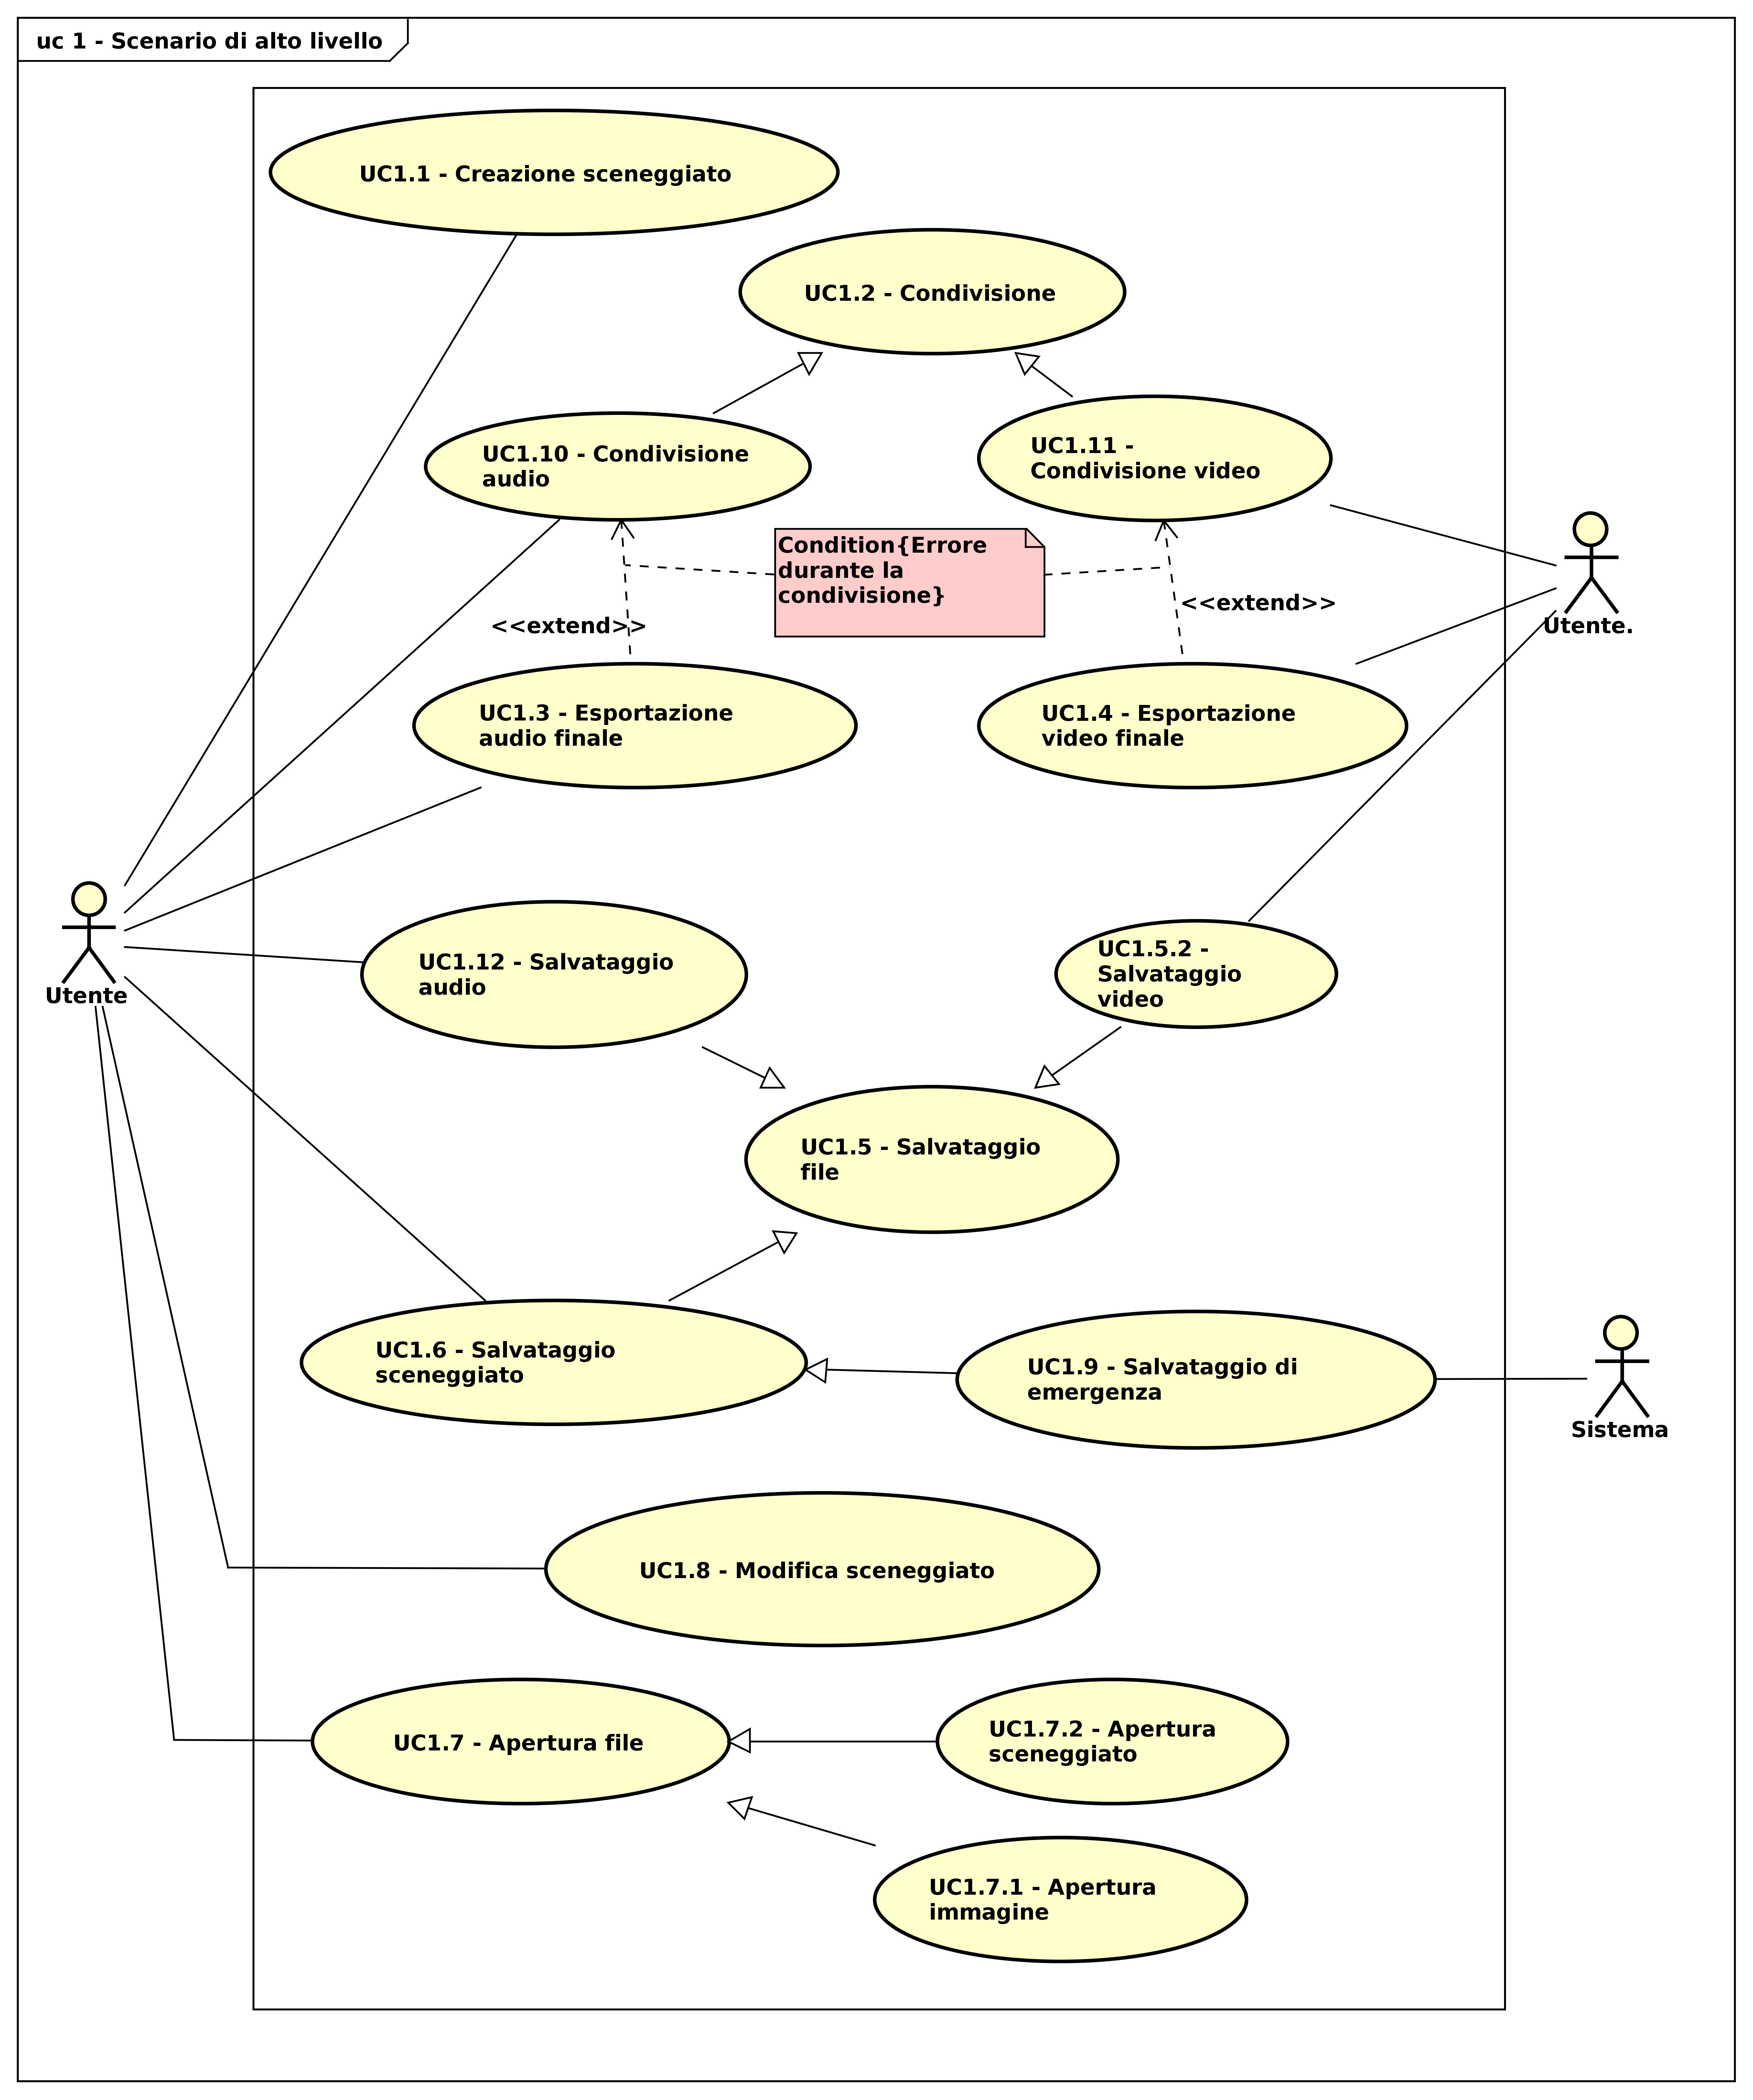
\includegraphics[scale=0.5]{immagini/uc1_scenario_alto_livello.png}
\captionsetup{labelfont=bf}
\caption{Caso d'uso UC1}
\end{figure}
\newpage


\subsection{Caso d'uso UC1.1: Creazione sceneggiato}
\label{sec:UC1.1}


\begin{itemize}
\item \textbf{Attore}: utente;
\item \textbf{Scopo e descrizione}: l'utente ha scelto di creare un nuovo sceneggiato. L'utente deve poter inserire i capitoli che lo costituiscono, caratterizzare i personaggi che vi fanno parte e poter scrivere le battute;
\item \textbf{Precondizione}: il sistema è pronto a creare un nuovo sceneggiato;
\item \textbf{Flusso principale degli eventi}:
\begin{enumerate}
\item L'utente può assegnare un titolo allo sceneggiato (UC1.1.6);
\item L'utente può creare un nuovo personaggio dello sceneggiato (UC1.1.1);
\item L'utente può modificare o cancellare un personaggio (UC1.1.7, UC1.1.8);
\item L'utente può creare un nuovo capitolo (UC1.1.2);
\item L'utente può modificare un capitolo (UC1.1.3);
\item L'utente può riordinare i capitoli alterandone la sequenza (UC1.1.4);
\item L'utente può cancellare un capitolo (UC1.1.5).
\end{enumerate}
\item \textbf{Postcondizione}: l'applicazione ha creato un nuovo sceneggiato.
\end{itemize}

\begin{figure}[htbp]
\centering
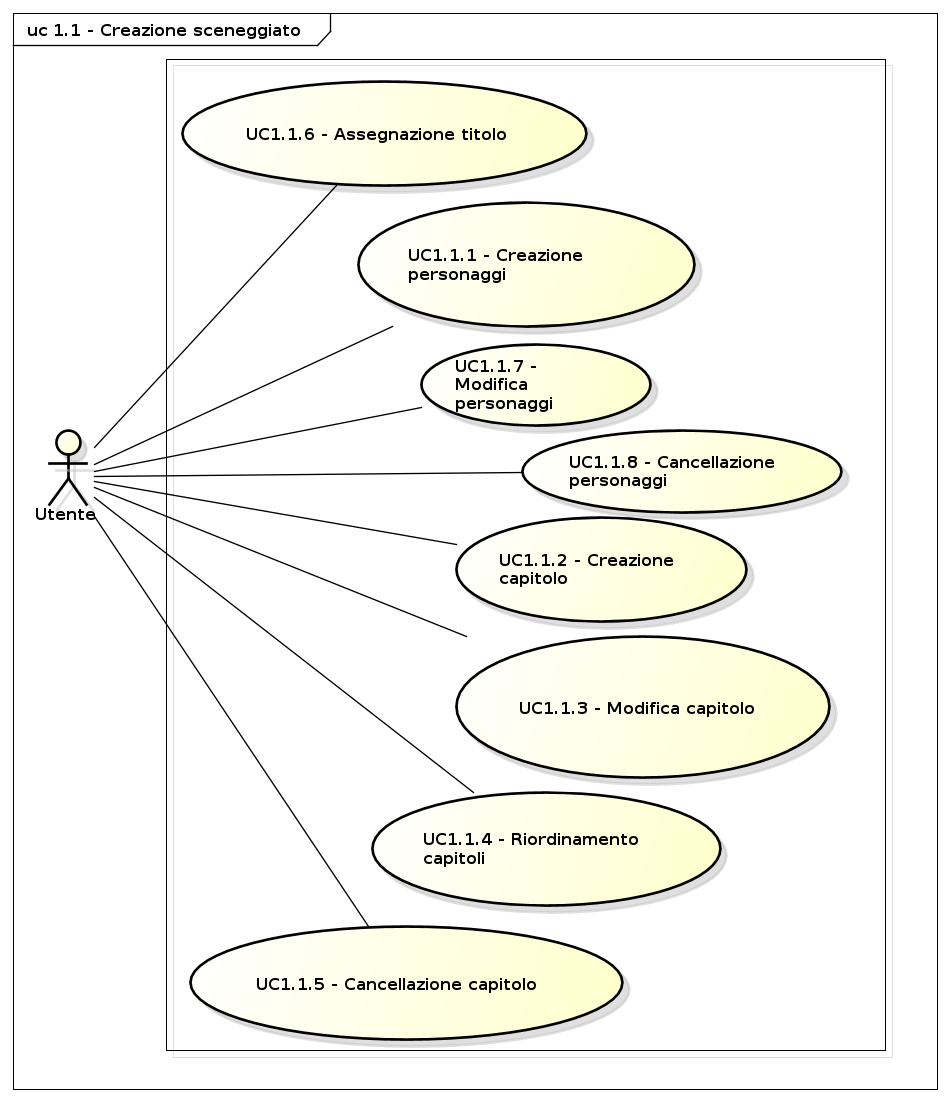
\includegraphics[scale=0.5]{immagini/uc1_1_creazione_sceneggiato.png}
\captionsetup{labelfont=bf}
\caption{Caso d'uso UC1.1}
\end{figure}
\newpage

\subsection{Caso d'uso UC1.1.1: Creazione personaggi}
\label{sec:UC1.1.1}

\begin{itemize}
\item \textbf{Attore}: utente;
\item \textbf{Scopo e descrizione}: l'utente può creare un nuovo personaggio per il suo sceneggiato associandoci nome, \textit{avatar\G} e voce;
\item \textbf{Precondizione}: il sistema è pronto a creare un nuovo personaggio;
\item \textbf{Flusso principale degli eventi}:
\begin{enumerate}
\item L'utente assegna un nome al nuovo personaggio (UC1.1.1.1);
\item L'utente assegna un \textit{avatar} al nuovo personaggio, ossia l'immagine con cui il personaggio viene raffigurato nello sceneggiato (UC1.1.1.3);
\item L'utente assegna una voce (\textit{preset}\G) al nuovo personaggio (UC1.1.1.2);
\item L'utente può creare una nuova voce, che in seguito può essere assegnata al personaggio (UC1.1.1.4);
\item L'utente può modificare una voce già esistente, prima di assegnarla al personaggio (UC1.1.1.5).
\end{enumerate} 
\item \textbf{Scenari alternativi}: se il server di \AZIENDA\ non è raggiungibile, è possibile assegnare al personaggio una voce predefinita di sistema;
\item \textbf{Postcondizione}: il sistema crea un nuovo personaggio.
\end{itemize}

\begin{figure}[htbp]
\centering
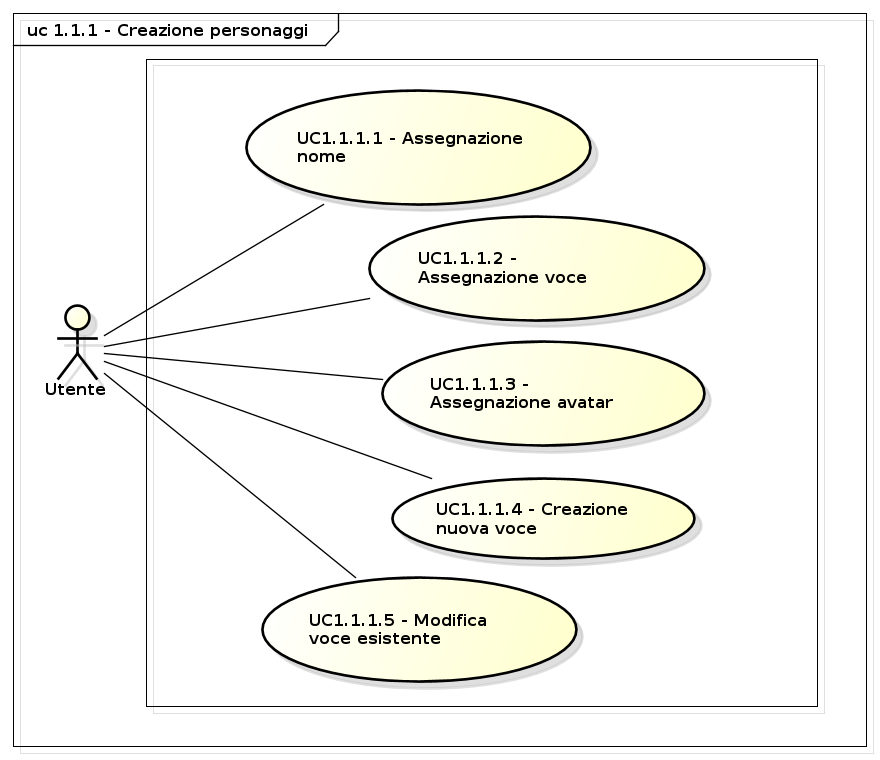
\includegraphics[scale=0.5]{immagini/uc1_1_1_creazione_personaggi.png}
\captionsetup{labelfont=bf}
\caption{Caso d'uso UC1.1.1}
\end{figure}
\newpage

\subsection{Caso d'uso UC1.1.1.2: Assegnazione voce}
\label{sec:UC1.1.1.2}
\begin{itemize}
\item \textbf{Attore}: utente;
\item \textbf{Scopo e descrizione}: l'utente assegna a un personaggio una fra le voci disponibili; 
\item \textbf{Precondizione}: il sistema è pronto a ricevere la selezione di una voce;
\item \textbf{Flusso principale degli eventi}:
\begin{enumerate}
\item L'utente può navigare tra le voci disponibili (UC1.1.1.2.1);
\item L'utente seleziona una voce (UC1.1.1.2.2).
\end{enumerate}
\item \textbf{Postcondizione}: il sistema associa la voce selezionata al personaggio.
\end{itemize}

\subsection{Caso d'uso UC1.1.1.4: Creazione nuova voce}
\label{sec:UC1.1.1.4}

\begin{itemize}
\item \textbf{Attore}: utente;
\item \textbf{Scopo e descrizione}: l'utente può creare un nuova voce che può essere in seguito associata a un personaggio. La creazione di una voce avviene mediante la configurazione di un insieme di effetti e parametri;
\item \textbf{Precondizione}: il sistema è pronto a creare una nuova voce e ha caricato i parametri richiesti;
\item \textbf{Flusso principale degli eventi}:
\begin{enumerate}
\item L'utente seleziona una lingua (UC1.1.1.4.1);
\item L'utente seleziona il sesso della voce (UC1.1.1.4.2);
\item L'utente può modificare i parametri degli effetti applicabili (UC1.1.1.4.3);
\item L'utente può assegnare un nome alla voce (UC1.1.1.4.4).
\end{enumerate} 
\item \textbf{Scenari alternativi}: nel caso in cui il server di \AZIENDA\ non fosse raggiungibile, verranno rese disponibili le sole voci di sistema, alle quali non è possibile applicare effetti;
\item \textbf{Postcondizione}: il sistema memorizza la nuova voce.
\end{itemize}
\begin{figure}[htbp]
\centering
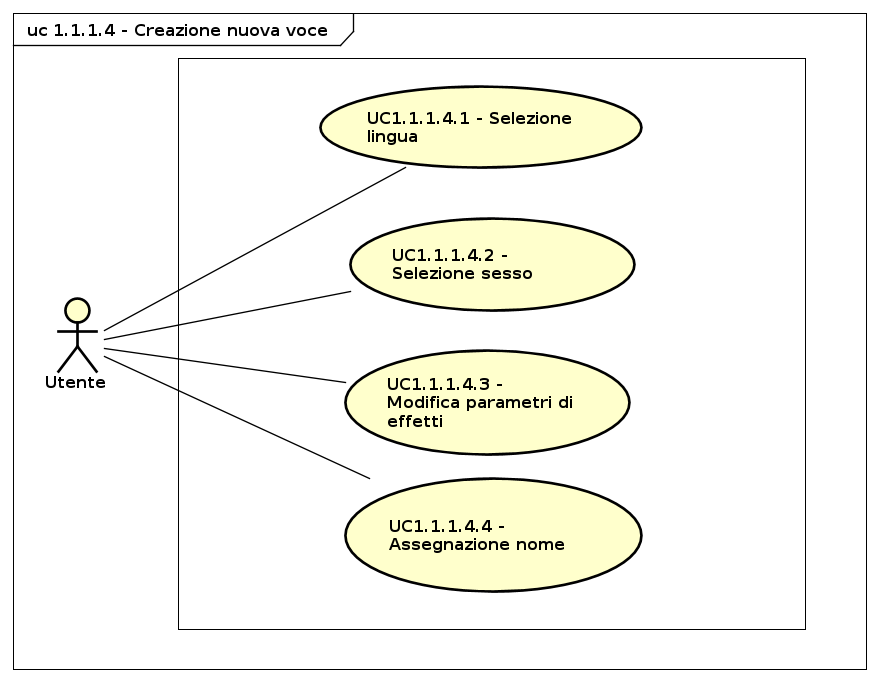
\includegraphics[scale=0.5]{immagini/uc1_1_1_4_creazione_nuova_voce.png}
\captionsetup{labelfont=bf}
\caption{Caso d'uso UC1.1.1.4}
\end{figure}
\newpage

\subsection{Caso d'uso UC1.1.2: Creazione capitolo}
\label{sec:UC1.1.2}

\begin{itemize}
\item \textbf{Attore}: utente;
\item \textbf{Scopo e descrizione}: l'utente può creare un capitolo dello sceneggiato. Nello specifico può inserire un'immagine di sfondo alla scena e scrivere le battute che i personaggi si scambiano in questo contesto. Ad ogni battuta possono essere applicati degli effetti, alcuni dei quali possono suggerire una determinata emozione;
\item \textbf{Precondizione}: l'utente ha creato uno sceneggiato e ci ha associato dei personaggi;
\item \textbf{Flusso principale degli eventi}:
\begin{enumerate}
\item L'utente assegna un titolo al capitolo (UC1.1.2.1);
\item L'utente crea lo sfondo, ossia il contesto visivo e sonoro in cui i personaggi si scambiano le battute (UC1.1.2.2);
\item L'utente scrive una nuova battuta (UC1.1.2.3);
\item L'utente può modificare una battuta (UC1.1.2.4);
\item L'utente può cancellare una battuta (UC1.1.2.5);
\item L'utente può associare alle battute degli effetti, che ne alterano il modo in cui sono sintetizzate (UC1.1.2.6);
\item L'utente può ascoltare un'anteprima del capitolo, per avere un riscontro di quanto creato in un certo momento (UC1.1.2.7);
\item L'utente può inserire un suono qualsiasi (per esempio un rumore ambientale), caricato dalla memoria o scelto fra una serie di suoni forniti (UC1.1.2.8). 
\end{enumerate} 
\item \textbf{Postcondizione}: è stato creato un capitolo dello sceneggiato;
\end{itemize}
\begin{figure}[htbp]
\centering
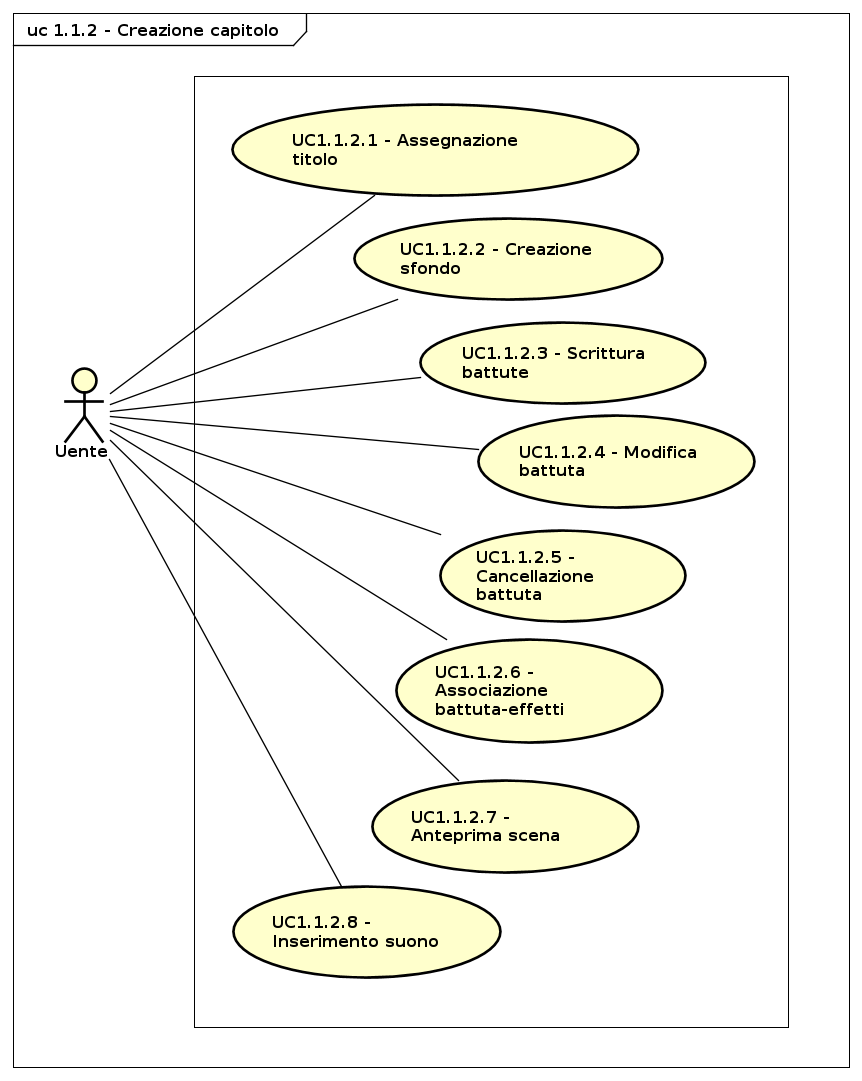
\includegraphics[scale=0.5]{immagini/uc1_1_2_creazione_capitolo.png}
\captionsetup{labelfont=bf}
\caption{Caso d'uso UC1.1.2}
\end{figure}
\newpage

\subsection{Caso d'uso UC1.1.2.2: Creazione sfondo}
\label{sec:UC1.1.2.2}

\begin{itemize}
\item \textbf{Attore}: utente;
\item \textbf{Scopo e descrizione}: l'utente può associare un'immagine e un audio di sottofondo a un capitolo creato;
\item \textbf{Precondizione}: l'utente ha creato un capitolo;
\item \textbf{Flusso principale degli eventi}:
\begin{enumerate}
\item L'utente assegna un'immagine di sfondo al capitolo, che può essere scelta da un insieme di immagini fornite, o caricata dall'utente (UC1.1.2.2.1);
\item L'utente assegna un audio di sottofondo al capitolo, scelto fra un insieme dato a disposizione, o caricato liberamente dall'utente (UC1.1.2.2.2);
\end{enumerate} 
\item \textbf{Postcondizione}: è stato creato lo sfondo di un capitolo dello sceneggiato;
\end{itemize}
\begin{figure}[htbp]
\centering
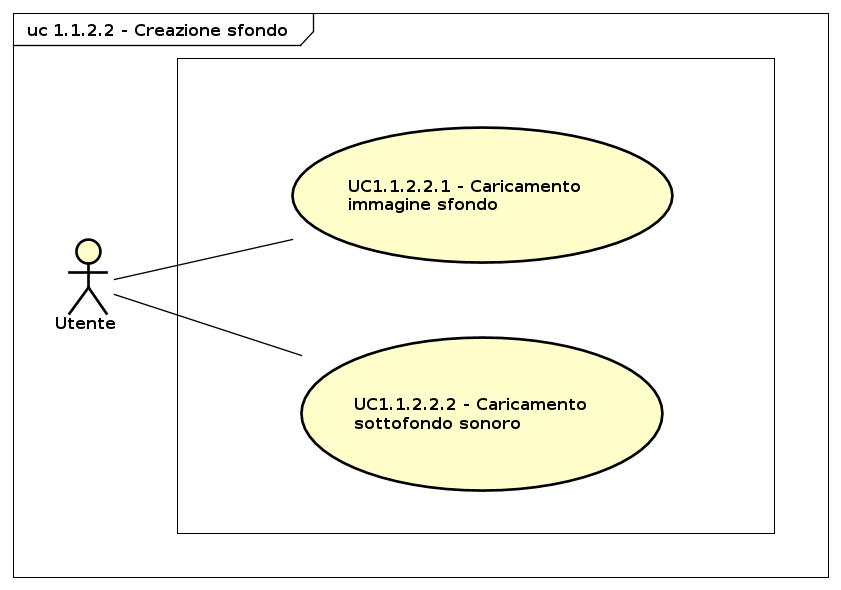
\includegraphics[scale=0.5]{immagini/uc1_1_2_2_creazione_sfondo.png}
\captionsetup{labelfont=bf}
\caption{Caso d'uso UC1.1.2.2}
\end{figure}
\newpage

\subsection{Caso d'uso UC1.1.2.3: Scrittura battute}
\label{sec:UC1.1.2.3}

\begin{itemize}
\item \textbf{Attore}: utente, modulo di sistema;
\item \textbf{Scopo e descrizione}: l'utente può digitare il testo di una nuova battuta e assegnarla a un personaggio tra quelli creati; il modulo di sistema provvede a convertire il testo inserito in SSML\G\ e a inviarlo al server di \AZIENDA; 
\item \textbf{Precondizione}: il sistema è pronto a ricevere il testo per la creazione di una nuova battuta;
\item \textbf{Flusso principale degli eventi}:
\begin{enumerate}
\item L'utente naviga tra i personaggi disponibili (UC1.1.2.3.1);
\item L'utente seleziona il personaggio a cui associare la battuta (UC1.1.2.3.2);
\item L'utente scrive il testo della nuova battuta (UC1.1.2.3.3);
\item Il modulo di sistema converte il testo della battuta scritta dall'utente in SSML (UC1.1.2.3.4).
\end{enumerate} 
\item \textbf{Postcondizione}: è stata creata una nuova battuta;
\end{itemize}
\begin{figure}[htbp]
\centering
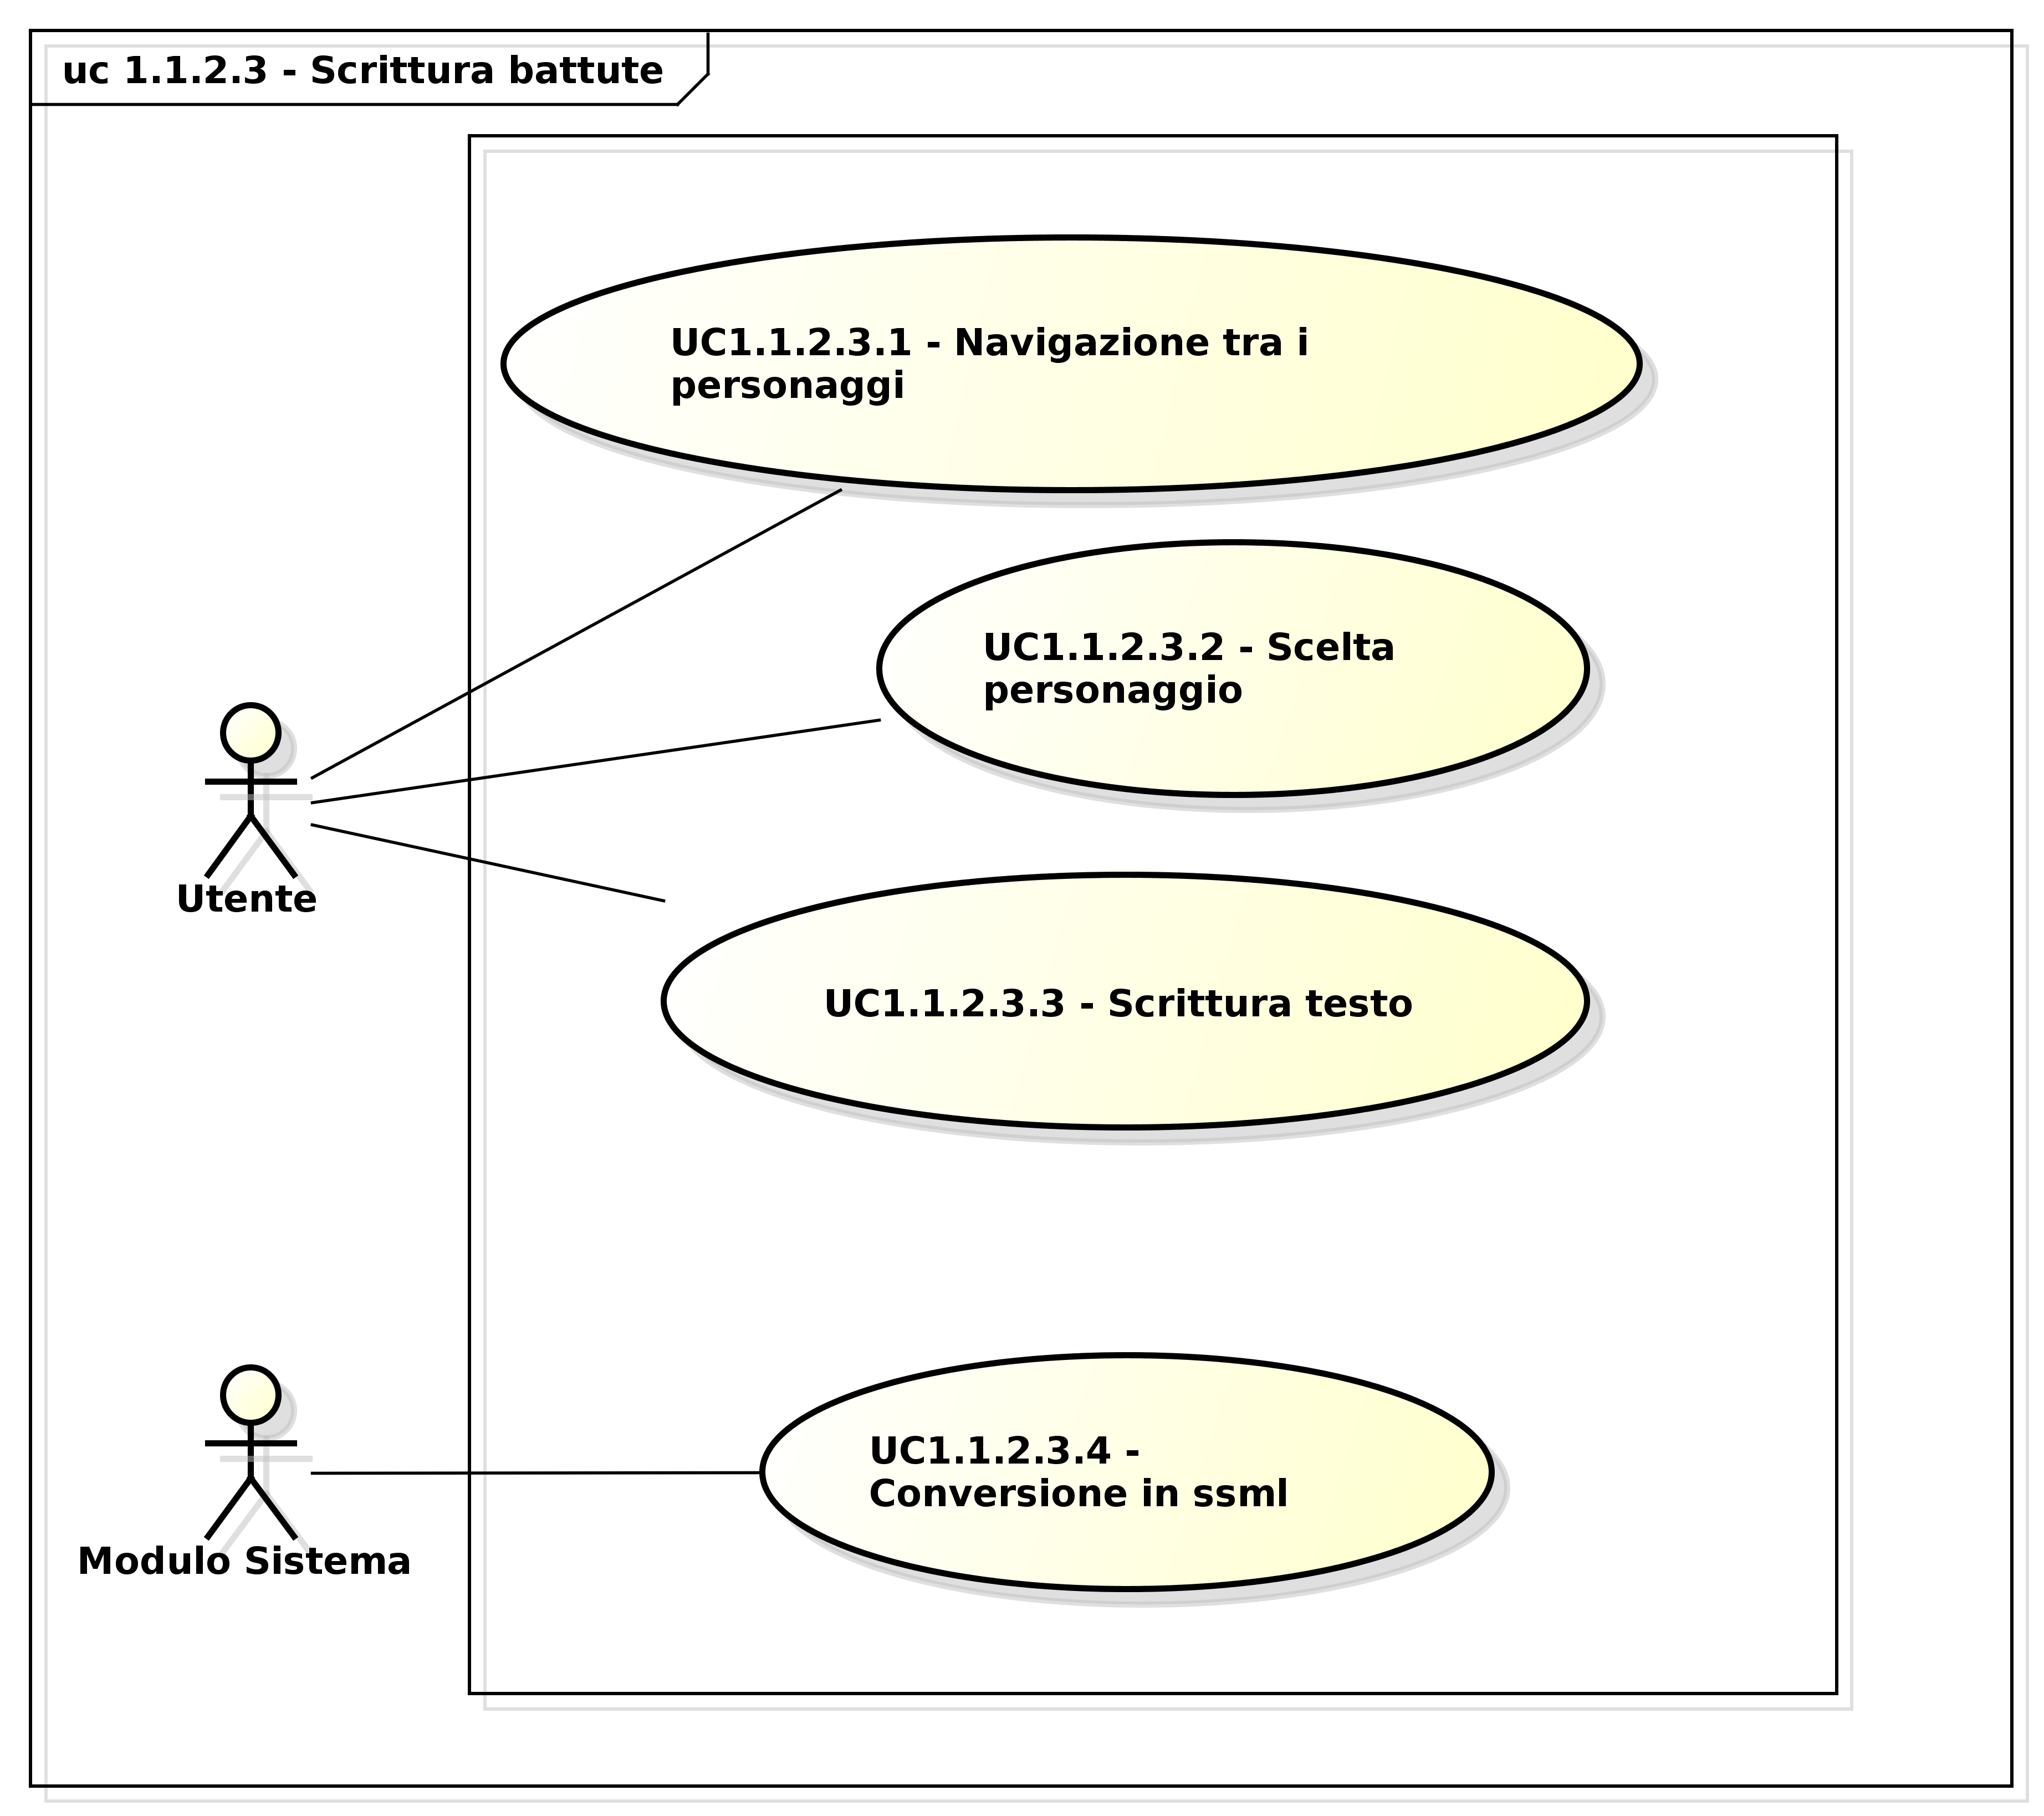
\includegraphics[scale=0.5]{immagini/uc1_1_2_3_scrittura_battute.png}
\captionsetup{labelfont=bf}
\caption{Caso d'uso UC1.1.2.3}
\end{figure}
\newpage

\subsection{Caso d'uso UC1.1.2.4: Modifica battuta}
\label{sec:UC1.1.2.4}

\begin{itemize}
\item \textbf{Attore}: utente, modulo di sistema;
\item \textbf{Scopo e descrizione}: avendo a disposizione almeno una battuta già creata, l'utente può decidere di modificarne: testo, personaggio, sentimento ed effetti associati;
\item \textbf{Precondizione}: almeno una battuta è già stata creata in precedenza;
\item \textbf{Flusso principale degli eventi}:
\begin{enumerate}
\item L'utente seleziona la battuta (UC1.1.2.4);
\item L'utente può cambiarne il testo (UC1.1.2.4.2);
\item L'utente può cambiarne il sentimento (UC1.1.2.4.3);
\item L'utente può cambiarne gli effetti associati, anche a basso livello (UC1.1.2.4.5);
\item L'utente può cambiarne il personaggio (UC1.1.2.4.4);
\item Il Modulo di Sistema converte la battuta in SSML\G\ (UC1.1.2.3.4);
\end{enumerate}
\item \textbf{Postcondizione}: è stata modificata una battuta già creata in precedenza.
\end{itemize}
\begin{figure}[htbp]
\centering
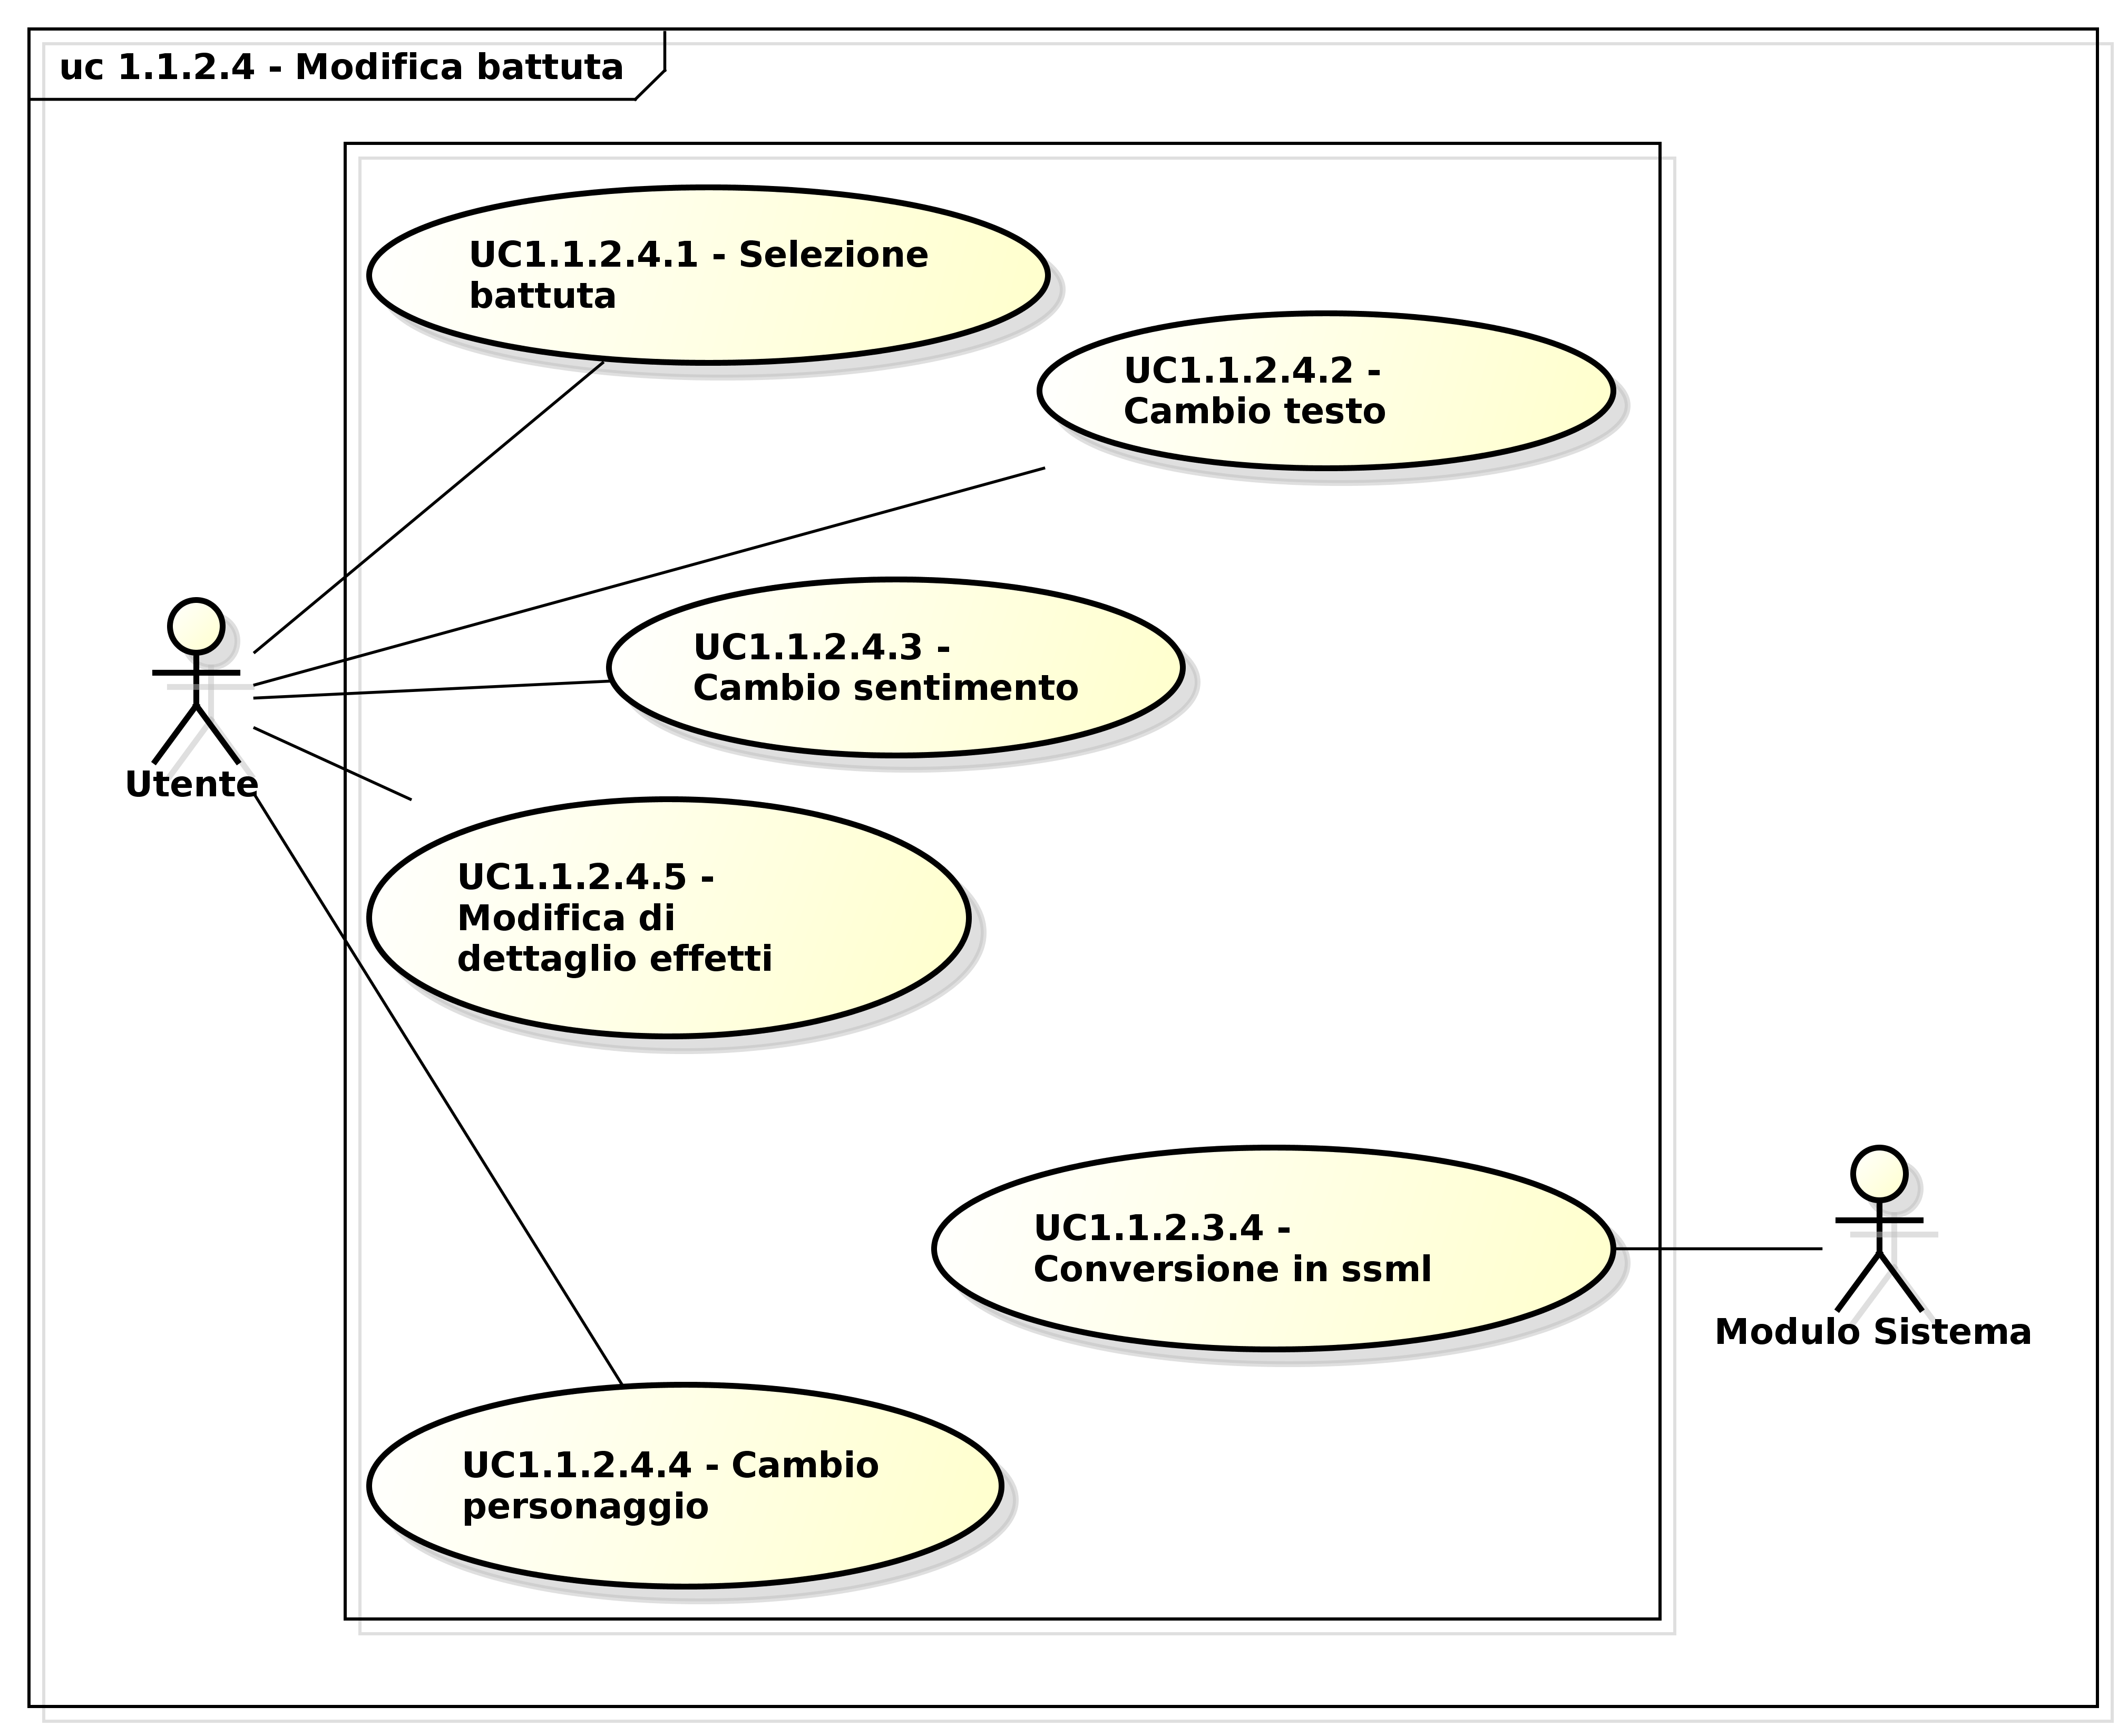
\includegraphics[scale=0.5]{immagini/uc1_1_2_4_modifica_battuta.png}
\captionsetup{labelfont=bf}
\caption{Caso d'uso UC1.1.2.4}
\end{figure}
\newpage

\subsection{Caso d'uso UC1.1.4: Associazione battuta-effetti}
\label{sec:UC1.1.4}

\begin{itemize}
\item \textbf{Attore}: utente, modulo di sistema;
\item \textbf{Scopo e descrizione}: avendo a disposizione almeno una battuta già creata, l'utente può modificare gli effetti associati e può testare le modifiche grazie a un'anteprima; 
\item \textbf{Precondizione}: almeno una battuta è già stata creata in precedenza;
\item \textbf{Flusso principale degli eventi}:
\begin{enumerate}
\item L'utente seleziona la battuta da modificare (UC1.1.2.6.1);
\item L'utente può scegliere se associare un sentimento alla battuta (UC1.1.2.6.3);
\item L'utente può scegliere di inserire delle pause nella battuta (UC1.1.2.6.4);
\item L'utente può scegliere se modificare gli effetti in dettaglio (UC1.1.2.6.5);
\item L'utente può scegliere se ascoltare un'anteprima della battuta (UC1.1.2.6.2);
\item Il Modulo di Sistema converte la battuta in SSML\G\ (UC1.1.2.6.6).
\end{enumerate}
\item \textbf{Postcondizione}: l'associazione battuta-effetti è avvenuta correttamente.
\end{itemize}
\begin{figure}[htbp]
\centering
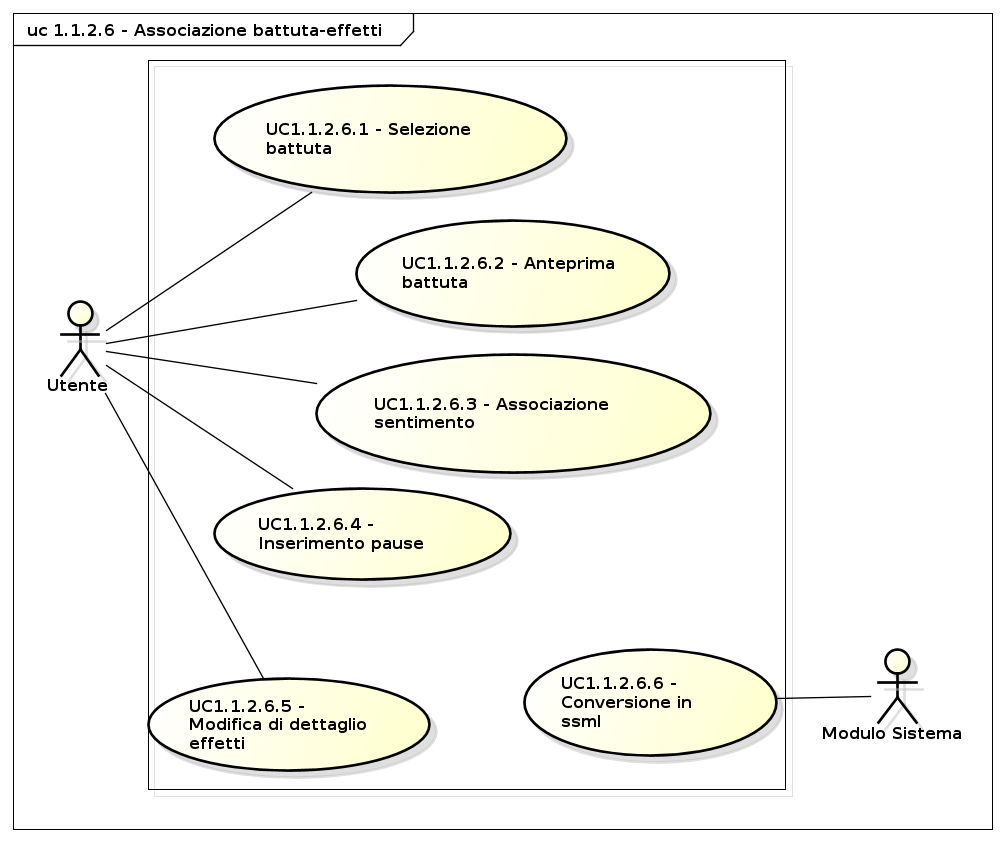
\includegraphics[scale=0.5]{immagini/uc1_1_2_6_associazione_battuta_effetti.png}
\captionsetup{labelfont=bf}
\caption{Caso d'uso UC1.1.2.6}
\end{figure}
\newpage

\subsection{Caso d'uso UC1.2: Condivisione}
\label{sec:UC1.2}

\begin{itemize}
\item \textbf{Attori}: utente, sistema;
\item \textbf{Scopo e descrizione}: l'utente può scegliere se condividere il \textit{file} relativo allo sceneggiato esportato in formato video o audio, selezionando uno tra gli strumenti di condivisione reperiti dal sistema;
\item \textbf{Precondizione}: lo sceneggiato è stato creato;
\item \textbf{Flusso principale degli eventi}:
\begin{enumerate}
\item L'utente sceglie se condividere lo sceneggiato in formato audio o video (UC1.2.4);
\item Il sistema reperisce la lista degli strumenti di condivisione presenti nel dispositivo (UC1.2.3);
\item L'utente può navigare tra gli elementi della lista sopracitata (UC1.2.1);
\item L'utente può scegliere uno tra gli elementi della lista (UC1.2.2).
\end{enumerate}
\item \textbf{Scenari alternativi}: se il dispositivo non possiede alcuno strumento di condivisione, è possibile unicamente creare un file audio o video da memorizzare nel dispositivo \textit{mobile}; 
\item \textbf{Postcondizione}: lo sceneggiato viene condiviso con successo in formato audio o video; 
\end{itemize}
\begin{figure}[htbp]
\centering
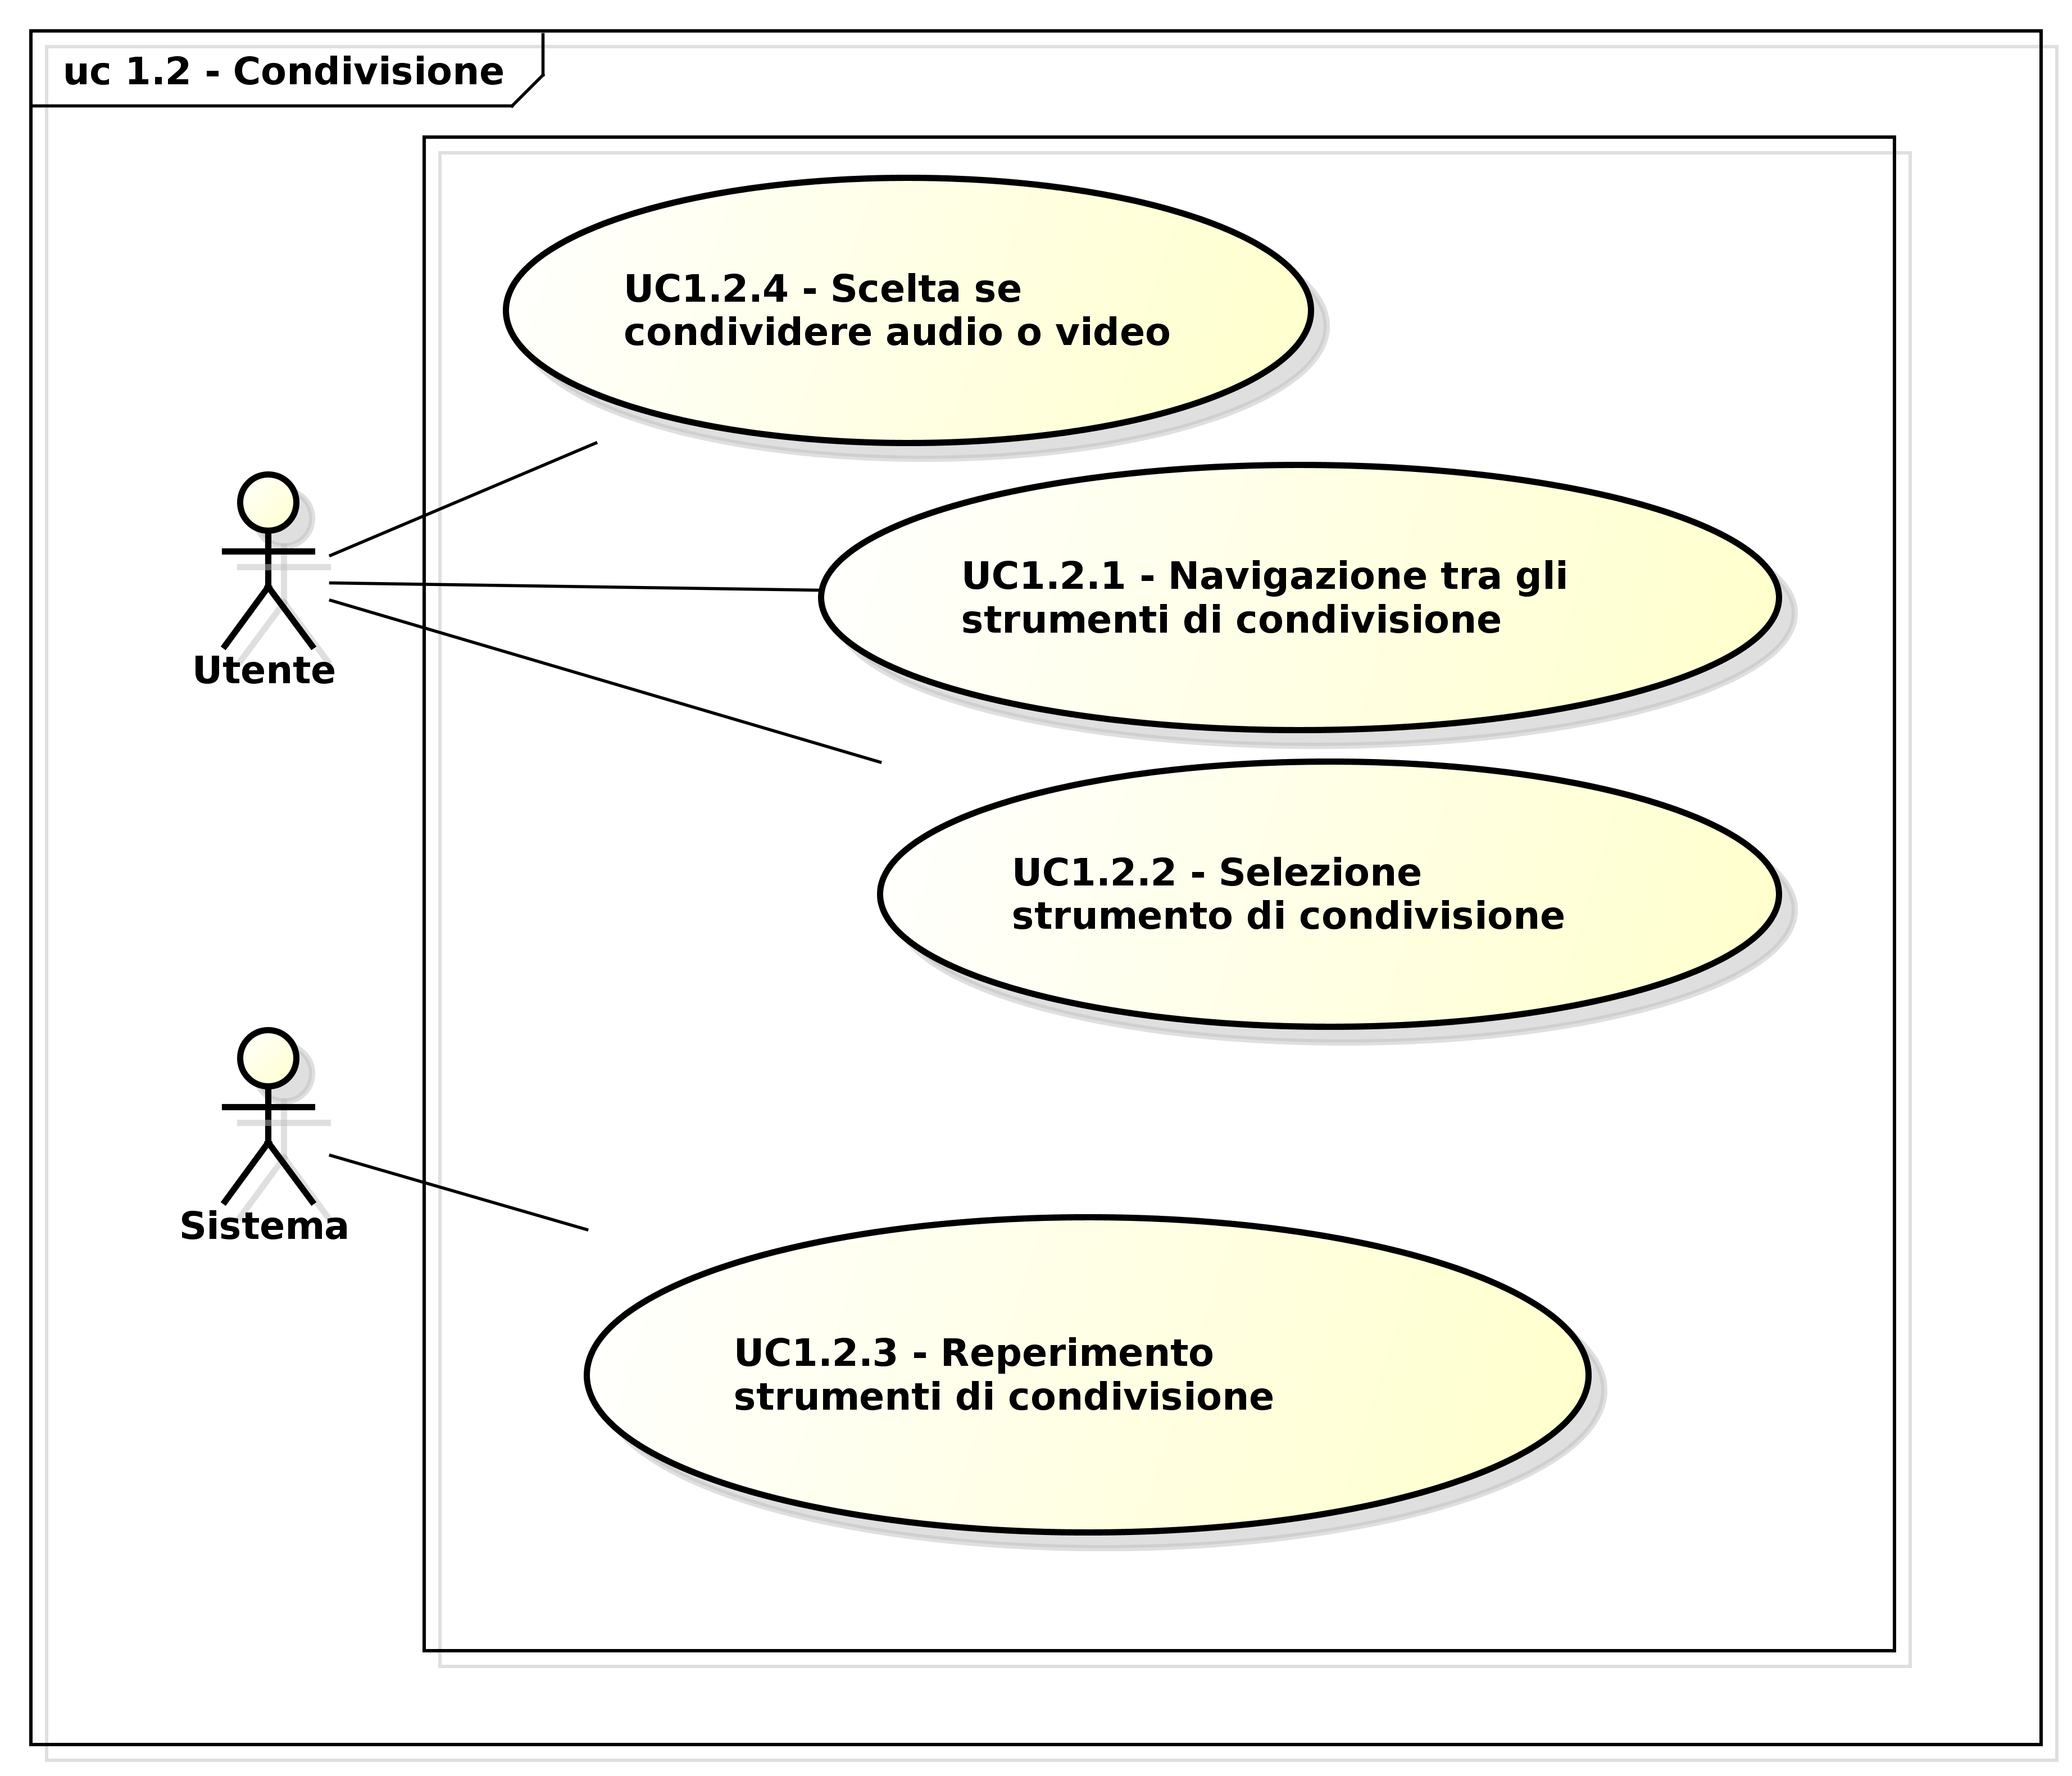
\includegraphics[scale=0.5]{immagini/uc1_2_condivisione.png}
\captionsetup{labelfont=bf}
\caption{Caso d'uso UC1.2}
\end{figure}
\newpage

\subsection{Caso d'uso UC1.3: Esportazione file audio}
\label{sec:UC1.3}

\begin{itemize}
\item \textbf{Attore}: utente;
\item \textbf{Scopo e descrizione}: l'utente può esportare lo sceneggiato in un \textit{file} audio, scegliendone il nome e il formato di esportazione;
\item \textbf{Precondizione}: il sistema è pronto a esportare uno sceneggiato correttamente formato;
\item \textbf{Flusso principale degli eventi}:
\begin{enumerate}
\item L'utente digita il nome del \textit{file} di esportazione (UC1.3.2);
\item L'utente seleziona il formato desiderato (UC1.3.1).
\end{enumerate}
\item \textbf{Postcondizione}: viene effettuata l'esportazione nel formato desiderato.  
\end{itemize}
\begin{figure}[htbp]
\centering
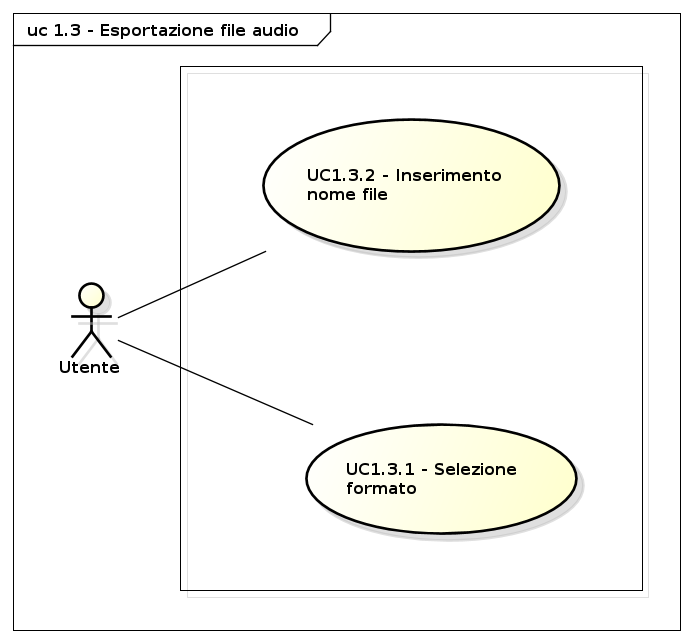
\includegraphics[scale=0.5]{immagini/uc1_3_esportazione_audio.png}
\captionsetup{labelfont=bf}
\caption{Caso d'uso UC1.3}
\end{figure}
\newpage

\subsection{Caso d'uso UC1.3: Esportazione file video}
\label{sec:UC1.3}

\begin{itemize}
\item \textbf{Attore}: utente;
\item \textbf{Scopo e descrizione}: l'utente può esportare lo sceneggiato in un \textit{file} video, scegliendone il nome e il formato di esportazione;
\item \textbf{Precondizione}: il sistema è pronto a esportare uno sceneggiato correttamente formato;
\item \textbf{Flusso principale degli eventi}:
\begin{enumerate}
\item L'utente digita il nome del \textit{file} di esportazione (UC1.4.2);
\item L'utente seleziona il formato desiderato (UC1.4.1).
\end{enumerate} 
\item \textbf{Postcondizione}: viene effettuata l'esportazione nel formato desiderato.  
\end{itemize}
\begin{figure}[htbp]
\centering
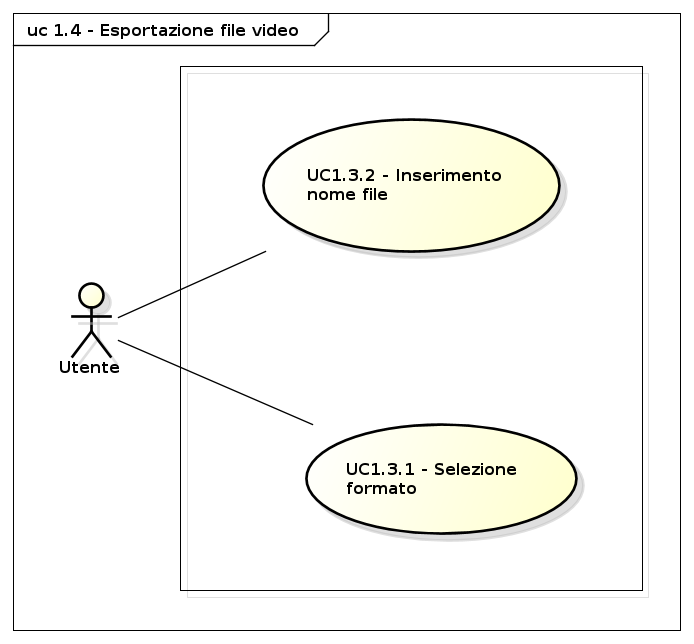
\includegraphics[scale=0.5]{immagini/uc1_4_esportazione_video.png}
\captionsetup{labelfont=bf}
\caption{Caso d'uso UC1.4}
\end{figure}
\newpage

\subsection{Caso d'uso UC1.5: Salvataggio file}
\label{sec:UC1.5}

\begin{itemize}
\item \textbf{Attori}: utente, sistema;
\item \textbf{Scopo e descrizione}: l'utente può salvare le modifiche apportate a uno sceneggiato; il sistema provvede al salvataggio effettivo reperendo la cartella di destinazione impostata di default;
\item \textbf{Precondizione}: il sistema è pronto a effettuare il salvataggio;
\item \textbf{Flusso principale degli eventi}:
\begin{enumerate}
\item Il sistema reperisce la cartella di default (UC1.5.1);
\item Il sistema effettua il salvataggio (UC1.5.2). 
\end{enumerate} 
\item \textbf{Scenari alternativi}: il sistema avverte l'utente in caso il salvataggio non andasse a buon fine (ad esempio a causa di mancanza di memoria disponibile) (UC1.5.3);
\item \textbf{Postcondizione}: il salvataggio viene effettuato correttamente. 
\end{itemize}
\begin{figure}[htbp]
\centering
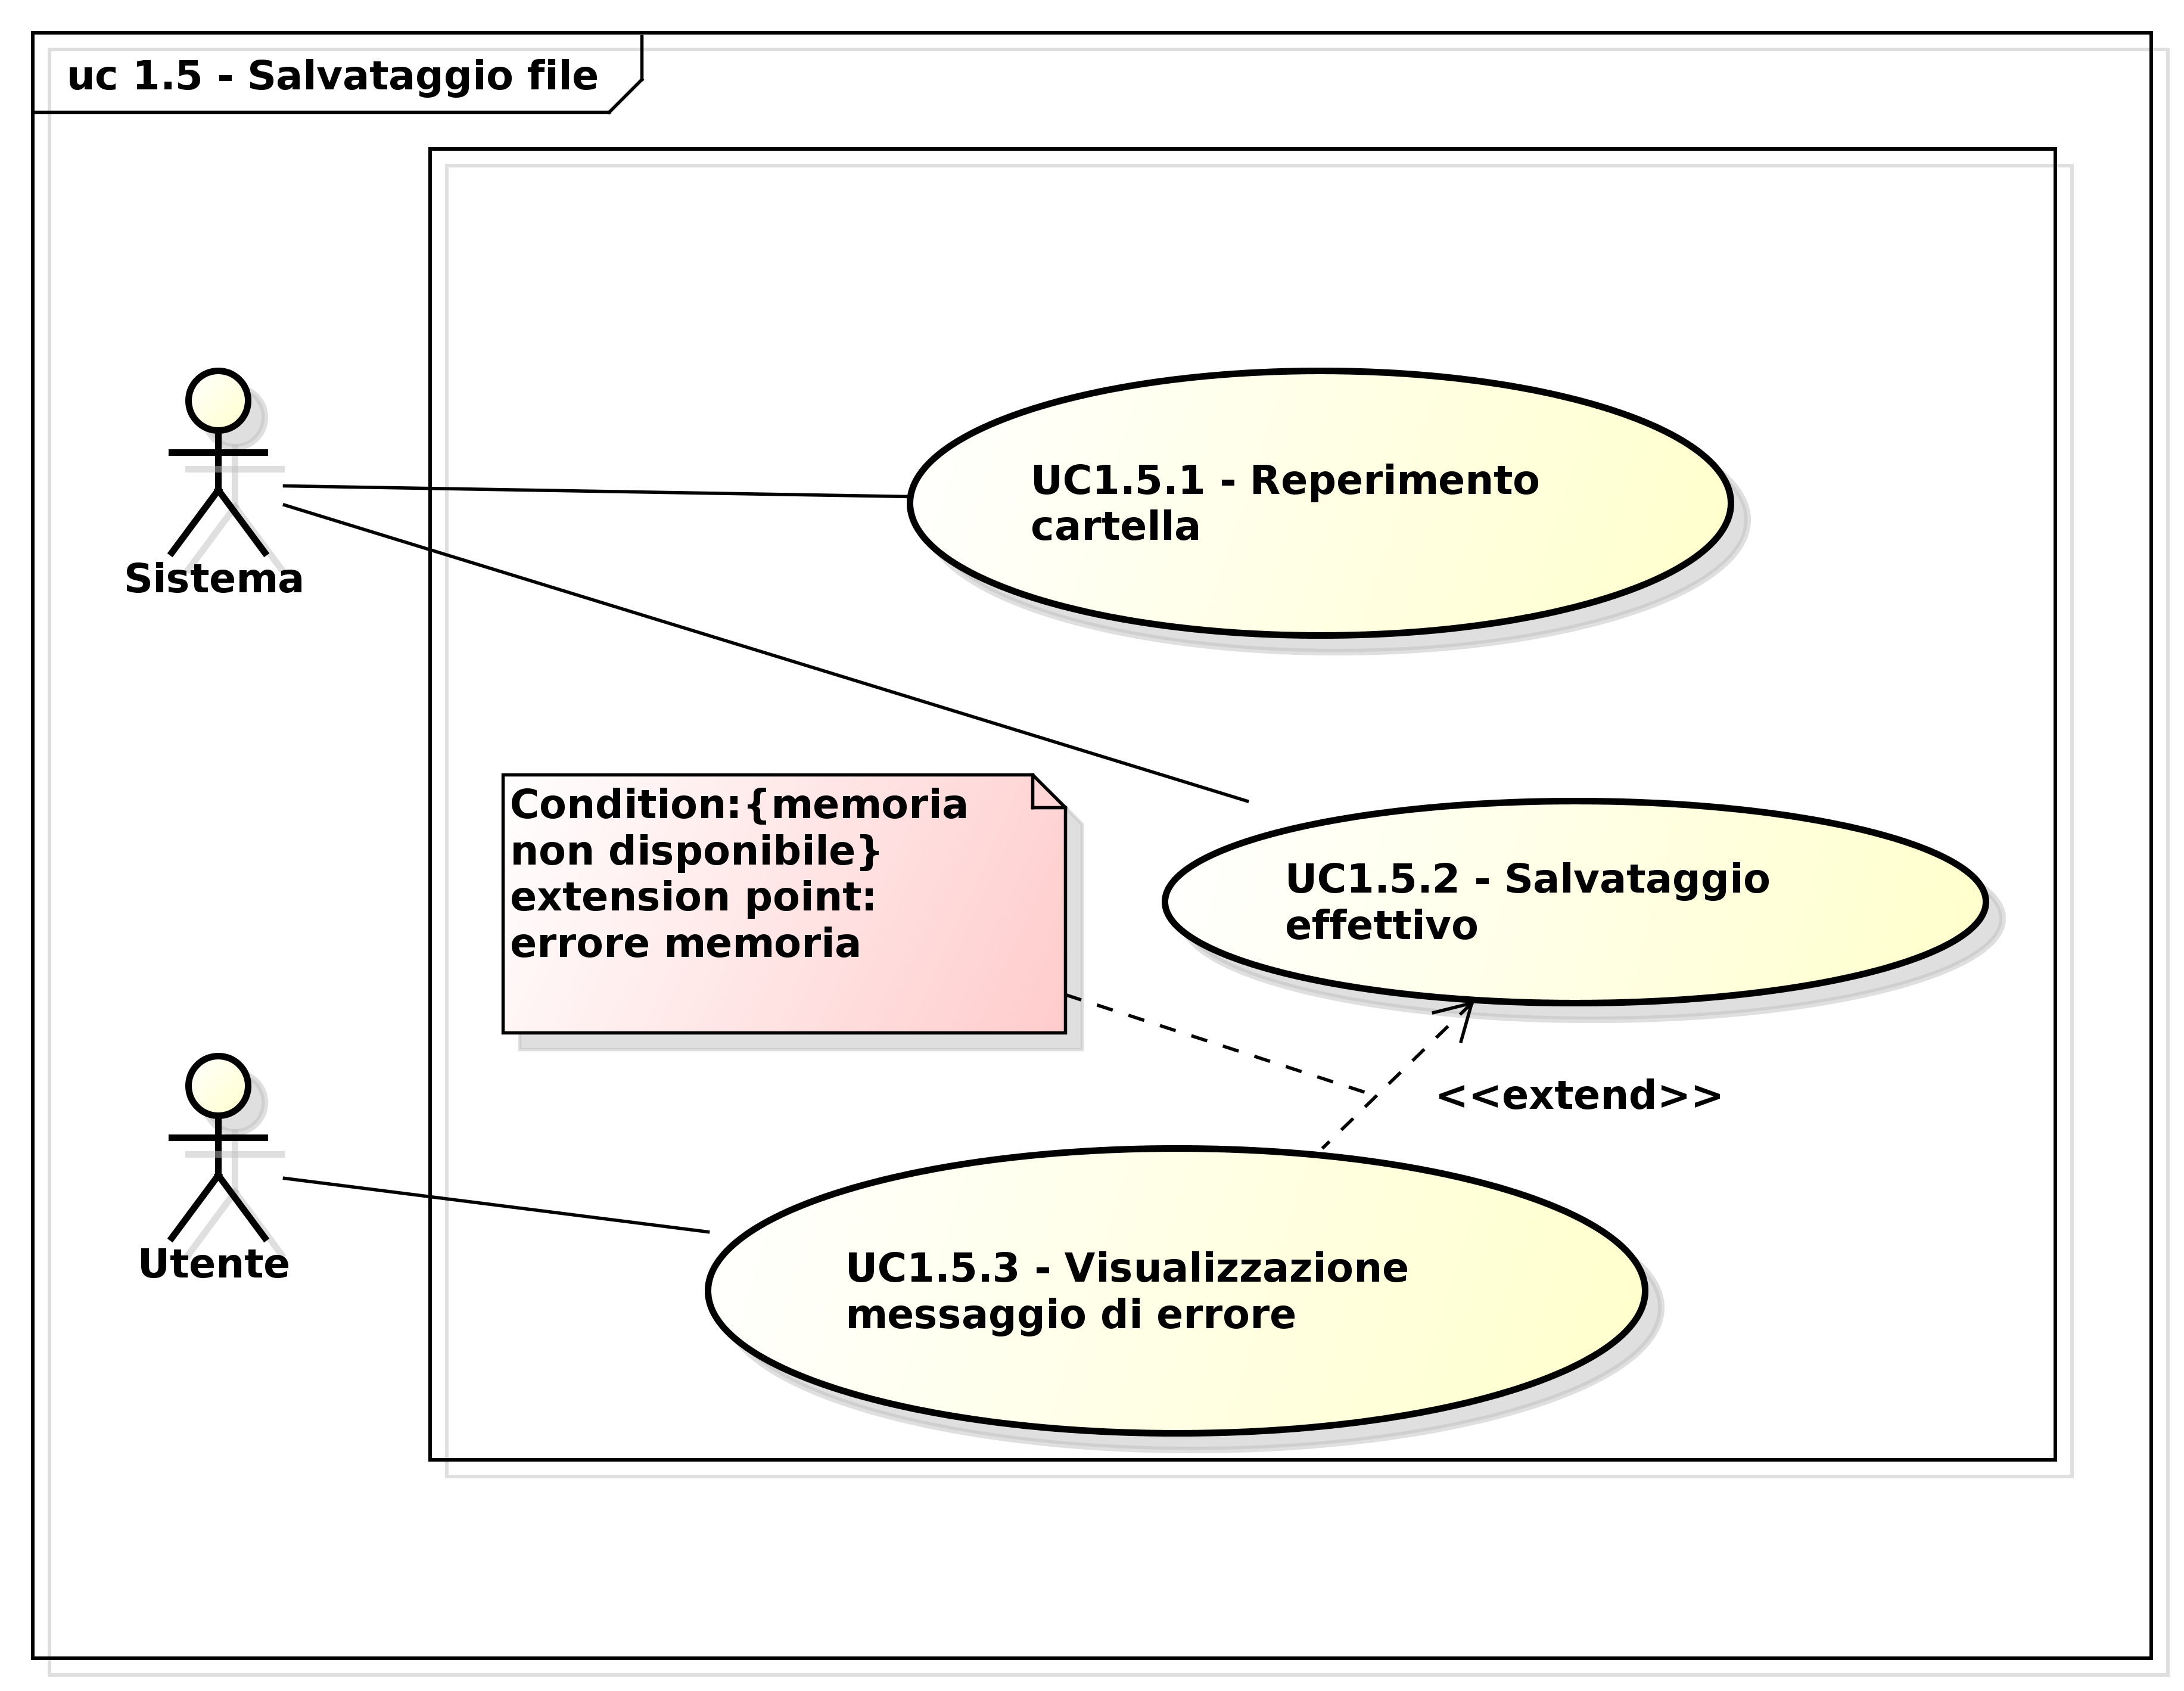
\includegraphics[scale=0.5]{immagini/uc1_5_salvataggio_file.png}
\captionsetup{labelfont=bf}
\caption{Caso d'uso UC1.5}
\end{figure}
\newpage

\subsection{Caso d'uso UC1.7: Apertura file}
\label{sec:UC1.7}

\begin{itemize}
\item \textbf{Attori}: utente;
\item \textbf{Scopo e descrizione}: navigando fra i \textit{file} di sistema, l'utente può selezionare un \textit{file} specifico da aprire;
\item \textbf{Precondizione}: il programma è avviato e viene richiesto il caricamento di un \textit{file};
\item \textbf{Flusso principale degli eventi}:
\begin{enumerate}
\item L'utente naviga fra i \textit{file} di sistema (UC1.7.0.1);
\item L'utente seleziona il \textit{file} da aprire (UC.1.7.0.2);
\item L'utente conferma l'apertura del \textit{file} selezionato (UC1.7.0.3).
\end{enumerate}
\item \textbf{Scenari alternativi}: il \textit{file} selezionato non è conforme alla tipologia di \textit{file} richiesto: in questo caso viene visualizzato un opportuno messaggio d'errore;
\item \textbf{Postcondizione}: il \textit{file} viene aperto correttamente.
\end{itemize}
\begin{figure}[htbp]
\centering
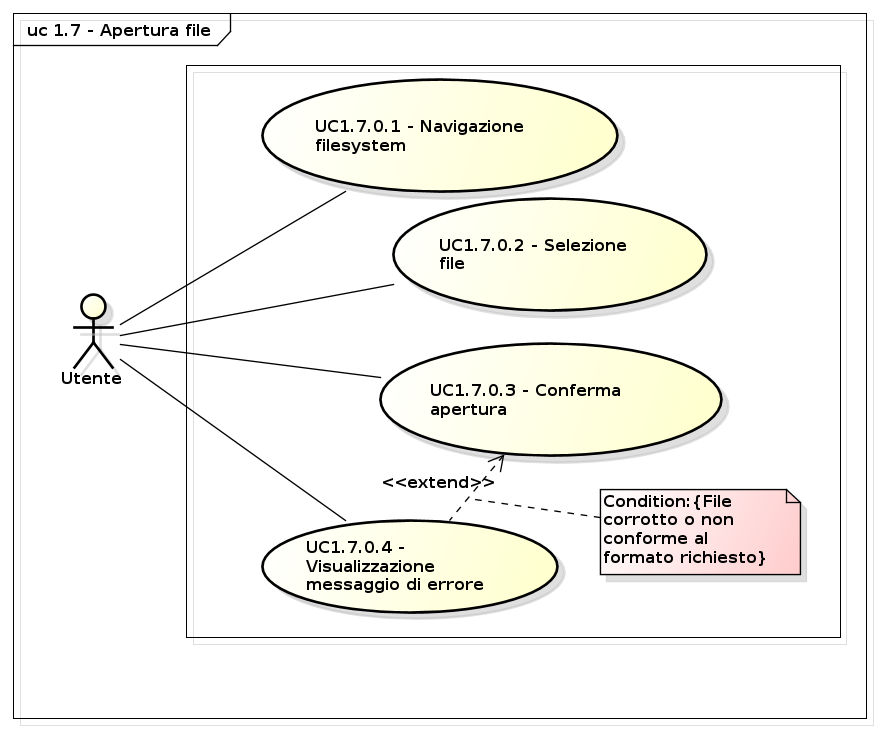
\includegraphics[scale=0.5]{immagini/uc1_7_apertura_file.png}
\captionsetup{labelfont=bf}
\caption{Caso d'uso UC1.7}
\end{figure}
\newpage

\subsection{Caso d'uso UC1.8: Modifica sceneggiato}
\label{sec:UC1.8}

\begin{itemize}
\item \textbf{Attori}: utente;
\item \textbf{Scopo e descrizione}: l'utente può aprire uno sceneggiato già creato e modificarlo;
\item \textbf{Precondizione}: esiste almeno uno sceneggiato creato in precedenza;
\item \textbf{Flusso principale degli eventi}:
\begin{enumerate}
\item L'utente apre lo sceneggiato da modificare (UC1.7.2);
\item L'utente può modificare un capitolo dello sceneggiato (UC1.8.1);
\item L'utente può avere un'anteprima dello sceneggiato appena modificato (UC1.8.2);
\end{enumerate}
\item \textbf{Postcondizione}: lo sceneggiato viene modificato correttamente.
\end{itemize}
\begin{figure}[htbp]
\centering
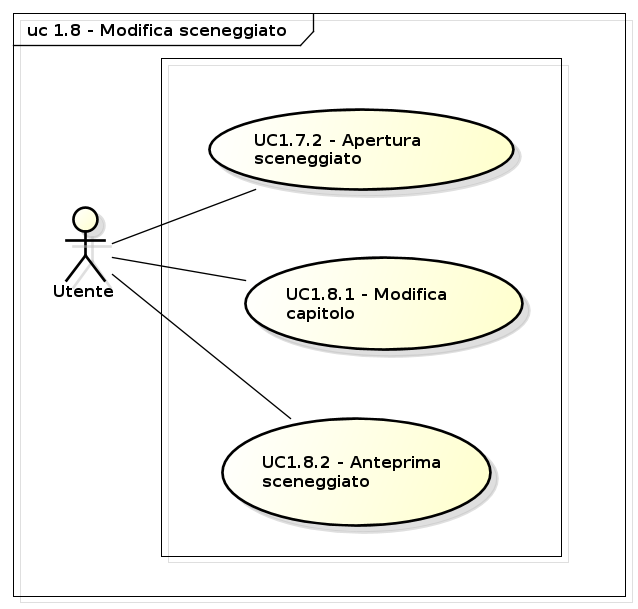
\includegraphics[scale=0.5]{immagini/uc1_8_modifica_sceneggiato.png}
\captionsetup{labelfont=bf}
\caption{Caso d'uso UC1.8}
\end{figure}
\newpage

\subsection{Caso d'uso UC1.8.1: Modifica capitolo}
\label{sec:UC1.8.1}

\begin{itemize}
\item \textbf{Attori}: utente;
\item \textbf{Scopo e descrizione}: l'utente può modificare un capitolo di uno sceneggiato già creato; nello specifico può modificarne lo sfondo, una o più battute, il titolo e i suoni di arricchimento;
\item \textbf{Precondizione}: nello sceneggiato è stato creato almeno un capitolo;
\item \textbf{Flusso principale degli eventi}:
\begin{enumerate}
\item L'utente seleziona il capitolo da modificare (UC1.8.1.1);
\item L'utente può vedere un'anteprima del capitolo (UC1.8.1.2);
\item L'utente può modificarne il titolo (UC1.8.1.4);
\item L'utente può modificarne lo sfondo (UC1.8.1.3);
\item L'utente può modificarne una battuta (UC1.1.2.4);
\item L'utente può cancellare una battuta del capitolo (UC1.1.2.5);
\item L'utente può inserire un nuovo suono di arricchimento o cancellarne uno inserito in precedenza (UC1.1.2.6, UC1.8.1.5).
\end{enumerate}
\item \textbf{Postcondizione}: il capitolo viene modificato correttamente.
\end{itemize}
\begin{figure}[htbp]
\centering
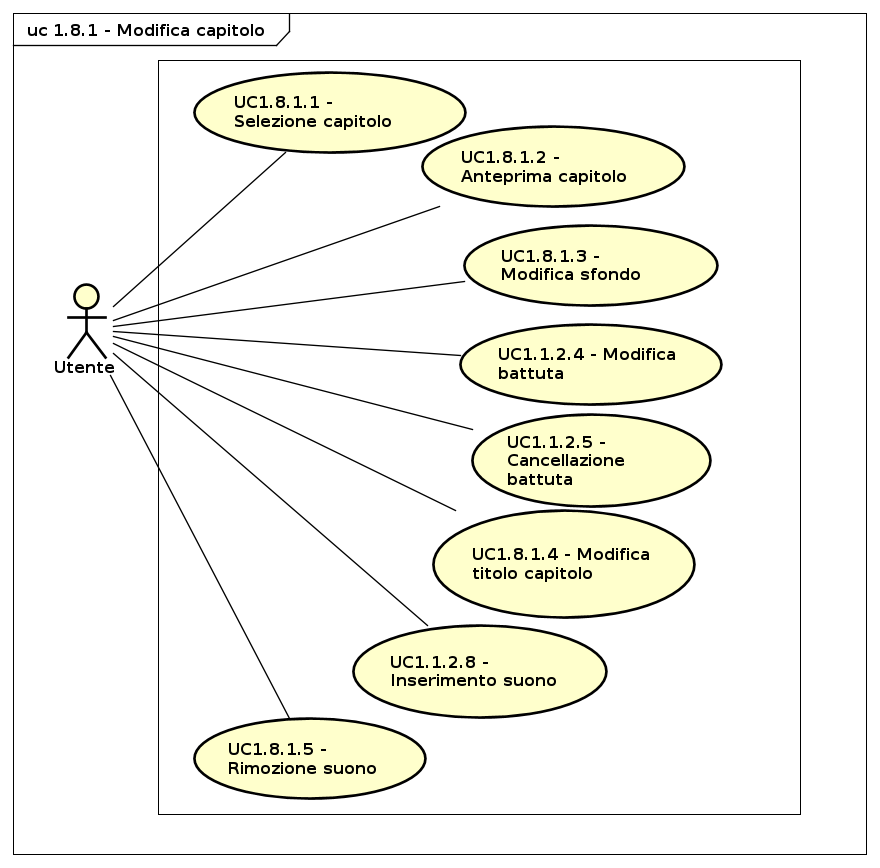
\includegraphics[scale=0.5]{immagini/uc1_8_1_modifica_capitolo.png}
\captionsetup{labelfont=bf}
\caption{Caso d'uso UC1.8.1}
\end{figure}
\newpage

\subsection{Caso d'uso UC2: Configurazione alto livello}
\label{sec:UC2}

\begin{itemize}
\item \textbf{Attori}: utente;
\item \textbf{Scopo e descrizione}: l'utente può creare nuovi \textit{preset}\G, modificando parametri ed effetti.  Inoltre può selezionare una nuova voce da impostare per il sistema e campionare la propria;
\item \textbf{Precondizione}: l'applicazione è stata avviata correttamente;
\item \textbf{Flusso principale degli eventi}:
\begin{enumerate}
\item L'utente può creare un nuovo \textit{preset} o modificarne uno già creato (UC2.1, UC2.5);
\item L'utente può testare il \textit{preset} creato (UC2.4); 
\item L'utente può selezionare una voce per il sistema (UC2.2);
\item L'utente può campionare la sua voce (UC2.3).
\end{enumerate}
\item \textbf{Postcondizione}: l'applicazione agisce secondo le direttive dell'utente.
\end{itemize}
\begin{figure}[htbp]
\centering
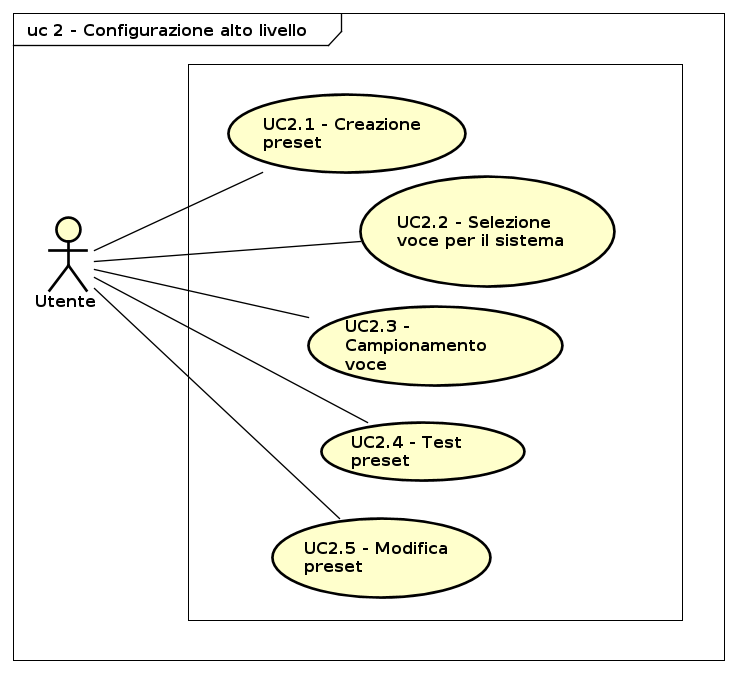
\includegraphics[scale=0.5]{immagini/uc2_configurazione_alto_livello.png}
\captionsetup{labelfont=bf}
\caption{Caso d'uso UC2}
\end{figure}
\newpage


\subsection{Caso d'uso UC2.1: Creazione preset}
\label{sec:UC2.1}

\begin{itemize}
\item \textbf{Attori}: utente, modulo di sistema;
\item \textbf{Scopo e descrizione}: dopo che il modulo di sistema ha reperito gli effetti disponibili, l'utente può navigare tra questi, selezionarli e associarli a voci; l'utente può infine salvare i cambiamenti apportati;
\item \textbf{Precondizione}: il sistema ha reperito gli effetti disponibili;
\item \textbf{Flusso principale degli eventi}:
\begin{enumerate}
\item Il modulo reperisce gli effetti (UC3.2);
\item L'utente può navigare tra gli effetti disponibili (UC2.1.1);
\item L'utente può settare dei parametri (UC2.1.2);
\item L'utente può salvare il \textit{preset}\G\ creato (UC2.1.3).
\end{enumerate}
\item \textbf{Postcondizione}: è stato salvato un \textit{preset} creato dall'utente.
\end{itemize}
\begin{figure}[htbp]
\centering
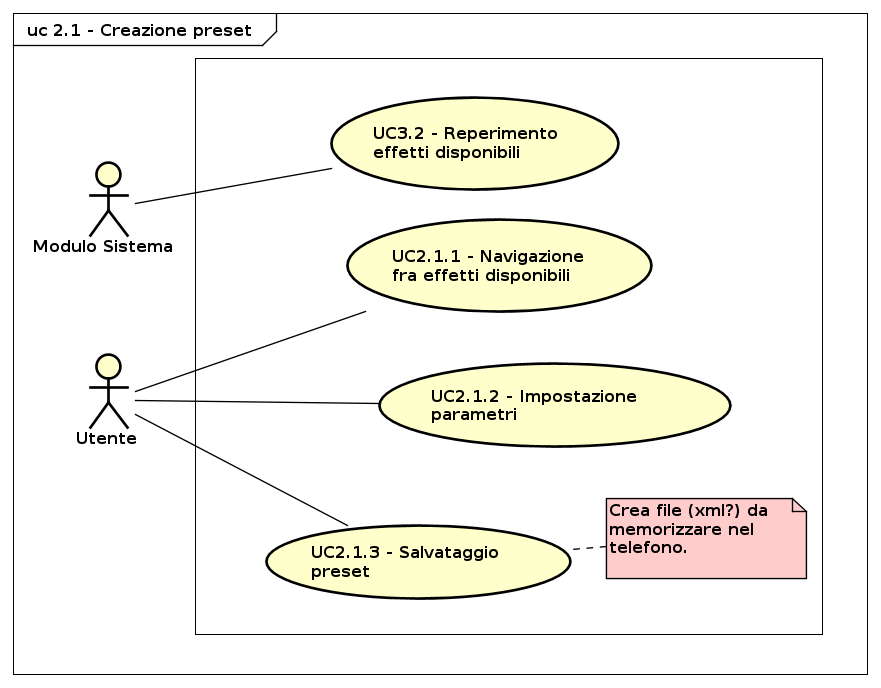
\includegraphics[scale=0.5]{immagini/uc2_1_creazione_preset.png}
\captionsetup{labelfont=bf}
\caption{Caso d'uso UC2.1}
\end{figure}
\newpage

\subsection{Caso d'uso UC2.2: Selezione voce per il sistema}
\label{sec:UC2.2}

\begin{itemize}
\item \textbf{Attori}: utente;
\item \textbf{Scopo e descrizione}: l'utente può impostare una delle voci disponibili come voce di default per il sistema, oppure può scegliere di crearne una nuova;
\item \textbf{Precondizione}: esistono delle voci disponibili;
\item \textbf{Postcondizione}: la voce è stata impostata correttamente.
\end{itemize}
\begin{figure}[htbp]
\centering
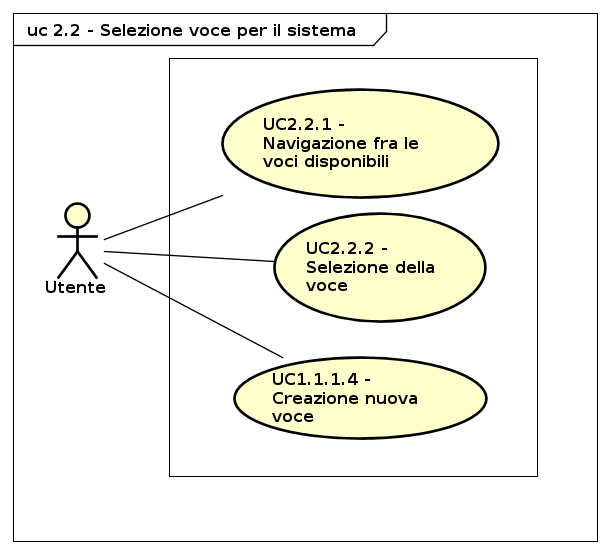
\includegraphics[scale=0.5]{immagini/uc2_2_selezione_voce_sistema.png}
\captionsetup{labelfont=bf}
\caption{Caso d'uso UC2.2}
\end{figure}
\newpage

\subsection{Caso d'uso UC2.3: Campionamento voce}
\label{sec:UC2.3}

\begin{itemize}
\item \textbf{Attori}: utente, applicazione;
\item \textbf{Scopo e descrizione}: l'utente può campionare la sua voce  eseguendo una procedura che prevede la lettura e la registrazione di frasi, che verranno inviate in formato audio dall'applicazione al server di \AZIENDA;
\item \textbf{Precondizione}: il sistema è pronto per il campionamento;
\item \textbf{Flusso principale degli eventi}:
\begin{enumerate}
\item L'utente effettua la login\G\ al servizio web di MIVOQ (UC2.3.4);
\item L'utente visualizza le frasi da leggere (UC2.3.1);
\item Viene registrata la lettura delle frasi (UC2.3.2);
\item L'applicazione invia la registrazione al server per il campionamento, per poi ricominciare dal punto 1. mostrando all'utente una nuova frase da leggere (UC2.3.3);
\item L'utente può decidere di terminare la sessione di campionamento, per continuare in un secondo momento.
\end{enumerate}
\item \textbf{Postcondizione}: il campionamento è andato a buon fine.
\end{itemize}
\begin{figure}[htbp]
\centering
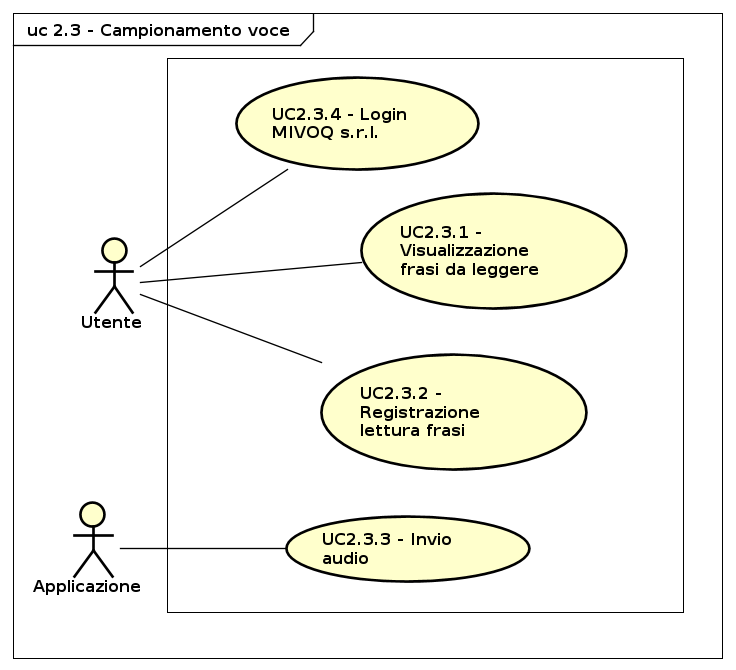
\includegraphics[scale=0.5]{immagini/uc2_3_campionamento_voce.png}
\captionsetup{labelfont=bf}
\caption{Caso d'uso UC2.3}
\end{figure}
\newpage

\subsection{Caso d'uso UC2.4: Test preset}
\label{sec:UC2.4}

\begin{itemize}
\item \textbf{Attori}: utente;
\item \textbf{Scopo e descrizione}: l'utente può ascoltare il \textit{preset}\G;
\item \textbf{Precondizione}: il \textit{preset} è stato creato correttamente;
\item \textbf{Postcondizione}: viene riprodotto l'audio di un testo di prova con il \textit{preset} associato.
\end{itemize}
\begin{figure}[htbp]
\centering
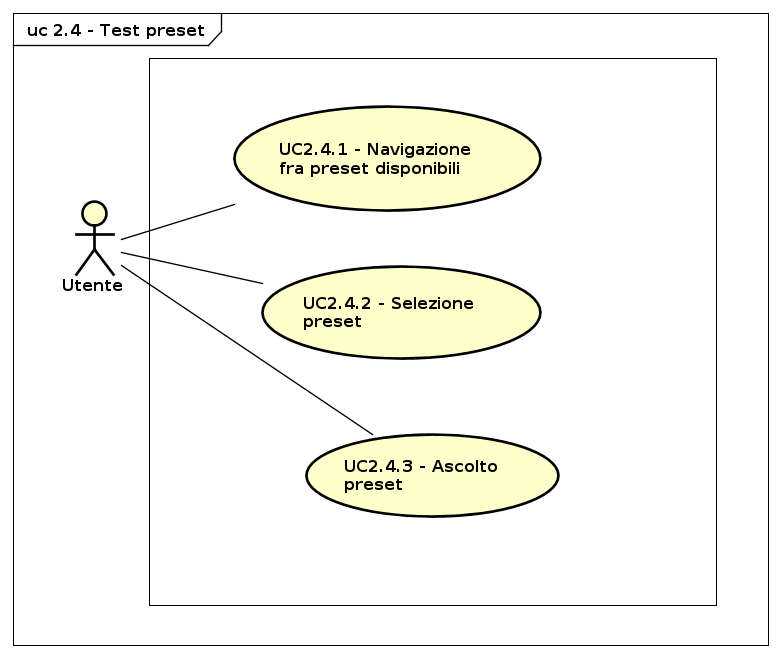
\includegraphics[scale=0.5]{immagini/uc2_4_test_preset.png}
\captionsetup{labelfont=bf}
\caption{Caso d'uso UC2.4}
\end{figure}
\newpage

\subsection{Caso d'uso UC2.5: Modifica preset}
\label{sec:UC2.5}

\begin{itemize}
\item \textbf{Attori}: utente;
\item \textbf{Scopo e descrizione}: l'utente può aprire un \textit{preset}\G\ già creato e modificarlo;
\item \textbf{Precondizione}: viene selezionato un \textit{preset} correttamente creato; 
\item \textbf{Flusso principale degli eventi}:
\begin{enumerate}
\item L'utente seleziona il \textit{preset} da modificare (UC2.5.1);
\item L'utente modifica i parametri del \textit{preset} (UC2.5.2);
\item L'utente salva le modifiche apportate (UC2.5.3).
\end{enumerate}
\item \textbf{Postcondizione}: il \textit{preset} viene modificato e salvato correttamente.
\end{itemize}
\begin{figure}[htbp]
\centering
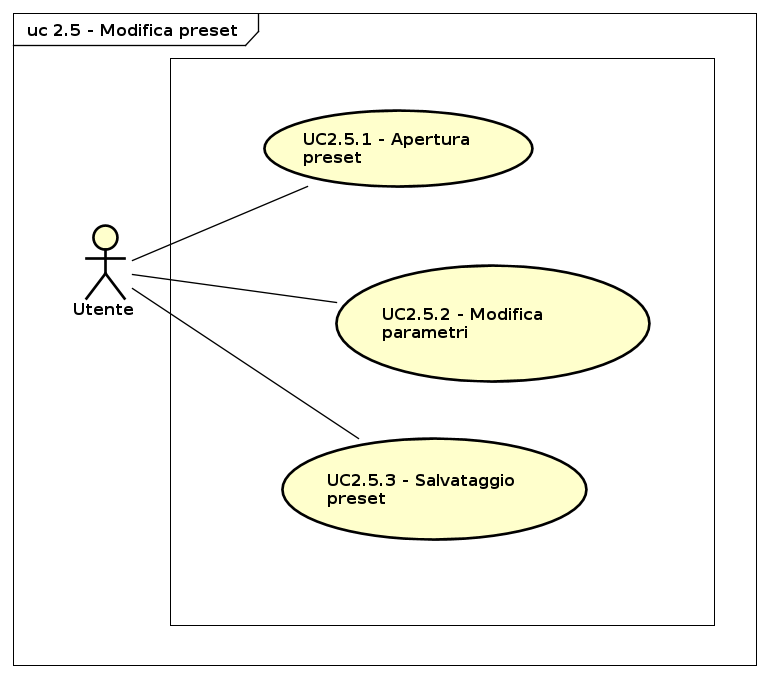
\includegraphics[scale=0.5]{immagini/uc2_5_modifica_preset.png}
\captionsetup{labelfont=bf}
\caption{Caso d'uso UC2.5}
\end{figure}
\newpage

\subsection{Caso d'uso UC3: Modulo di sistema alto livello}
\label{sec:UC3}

\begin{itemize}
\item \textbf{Attori}: modulo di sistema;
\item \textbf{Scopo e descrizione}: il modulo di sistema può reperire gli effetti e le voci disponibili comunicando con il server di \AZIENDA. Ogni comunicazione con il server avviene attraverso questa componente;
\item \textbf{Precondizione}: il modulo è pronto ad operare;
\item \textbf{Flusso principale degli eventi}:
\begin{enumerate}
\item Il modulo di sistema reperisce le voci disponibili (UC3.1);
\item Il modulo di sistema reperisce gli effetti disponibili (UC3.2);
\item Il modulo di sistema reperisce i \textit{file} audio (UC3.4);
\item Il modulo di sistema seleziona il \textit{preset}\G\ per il sistema (UC3.5);
\item Il modulo di sistema converte le battute in SSML\G\ (UC3.6);
\end{enumerate}
\item \textbf{Postcondizione}: il modulo svolge quanto richiesto;
\item \textbf{Generalizzazione}: il reperimento delle voci, degli effetti e la ricezione dell'audio sono azioni specifiche, che prevedono la comunicazione con il server di \AZIENDA.
\end{itemize}
\begin{figure}[htbp]
\centering
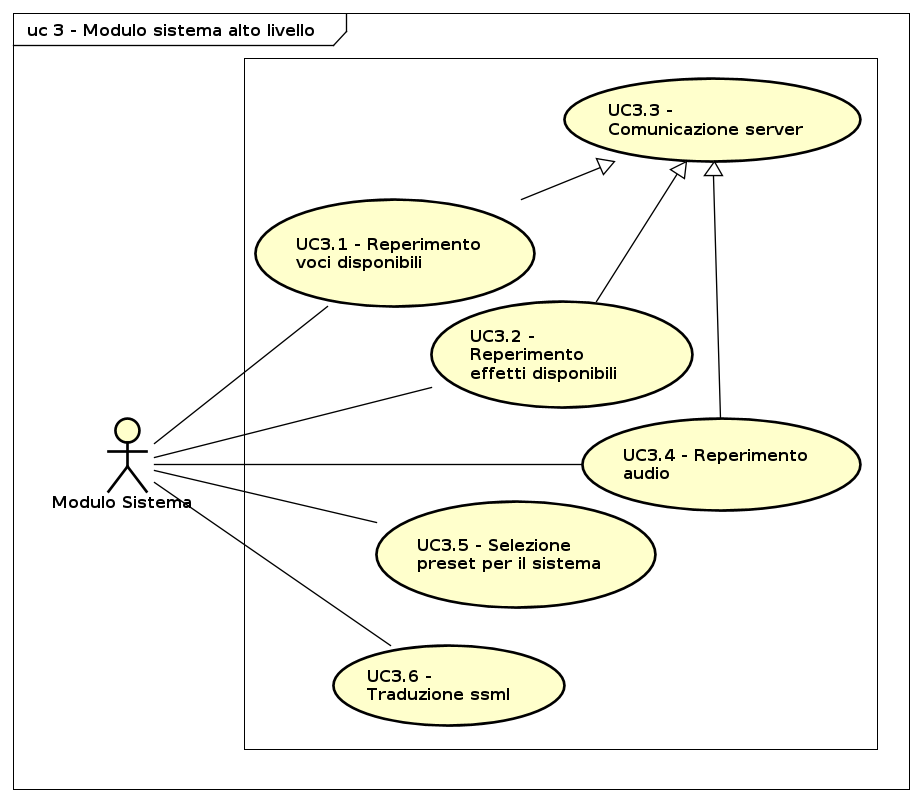
\includegraphics[scale=0.5]{immagini/uc3_modulo_sistema_alto_livello.png}
\captionsetup{labelfont=bf}
\caption{Caso d'uso UC3}
\end{figure}
\newpage

\subsection{Caso d'uso UC3.3: Comunicazione server}
\label{sec:UC3.3}

\begin{itemize}
\item \textbf{Attori}: modulo di sistema, utente;
\item \textbf{Scopo e descrizione}: il modulo di sistema crea una richiesta HTTP\G, la invia al server di \AZIENDA\ e attende una risposta da quest'ultimo; in caso di connessione alla rete assente viene mostrato all'utente un messaggio d'errore;
\item \textbf{Precondizione}: il modulo è pronto a comunicare con il server;
\item \textbf{Flusso principale degli eventi}:
\begin{enumerate}
\item Il modulo crea una richiesta HTTP (UC3.3.1);
\item Il modulo invia la richiesta HTTP creata (UC3.3.2);
\item Il modulo riceve una risposta dal server (UC3.3.3).
\end{enumerate}
\item \textbf{Scenari alternativi}: nel caso in cui non fosse possibile comunicare con il server a causa di connessione alla rete assente, il sistema avverte l'utente con un messaggio d'errore;  
\item \textbf{Postcondizione}: la comunicazione va a buon fine.
\end{itemize}
\begin{figure}[htbp]
\centering
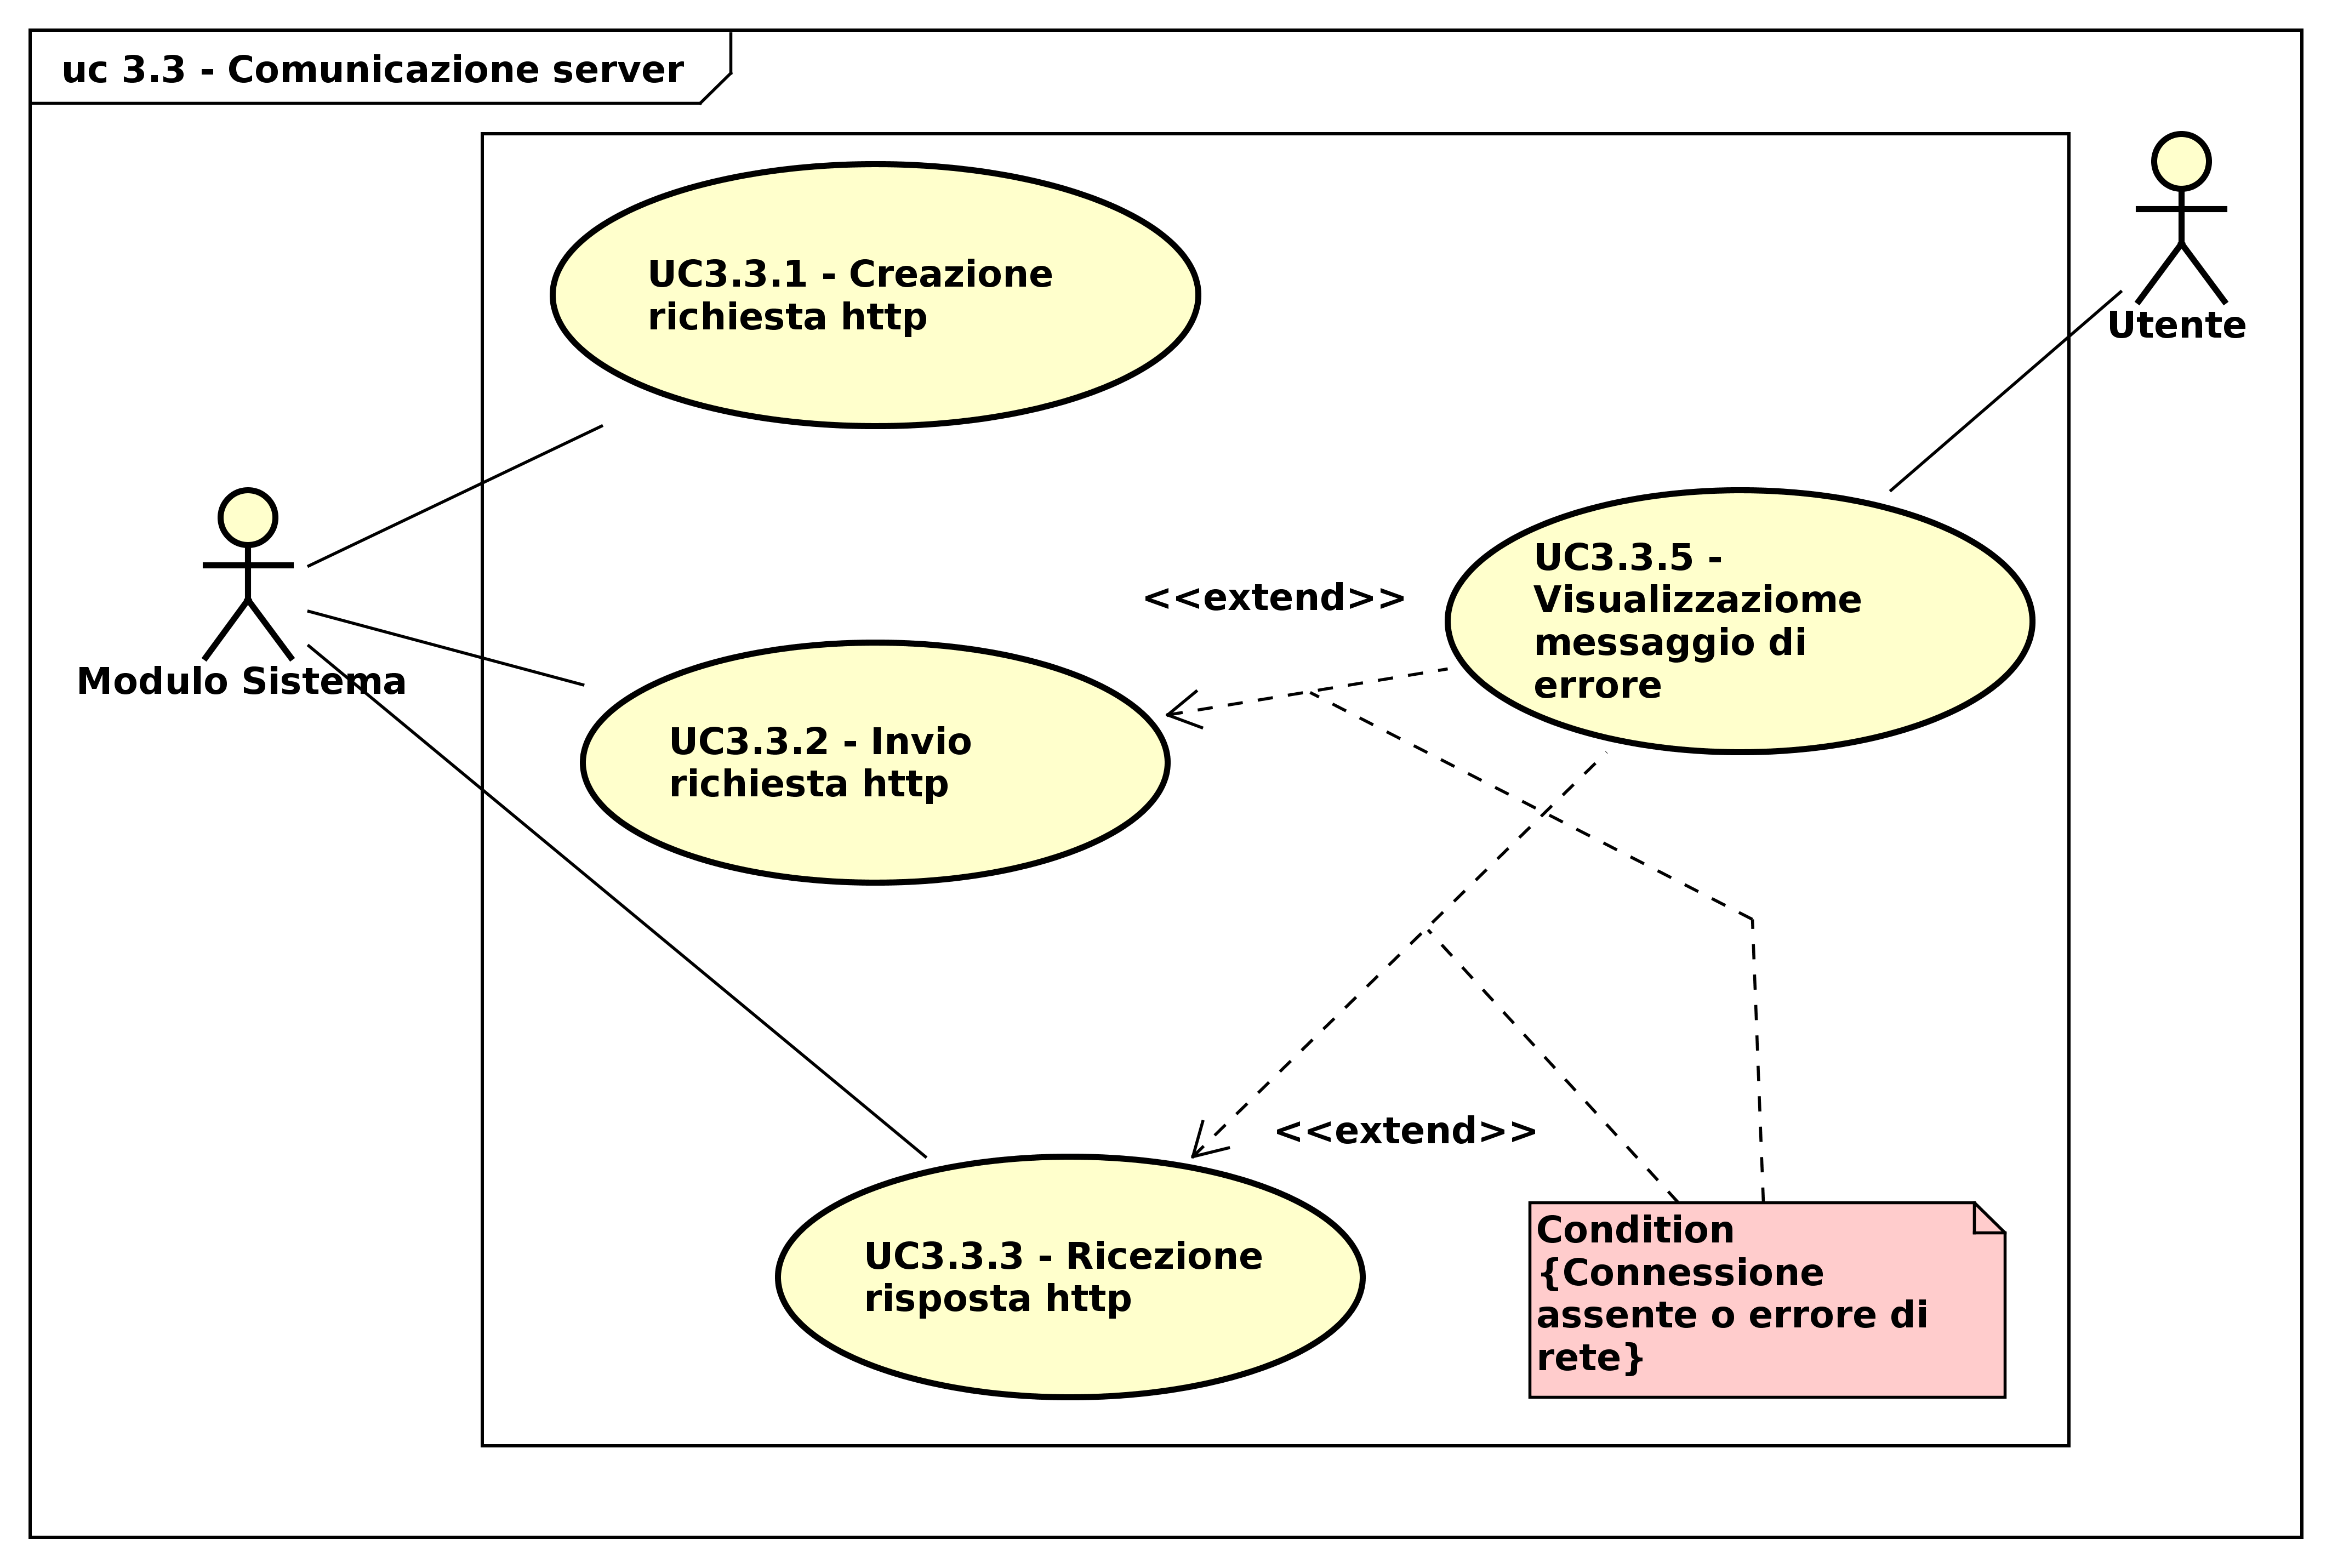
\includegraphics[scale=0.5]{immagini/uc3_3_comunicazione_server.png}
\captionsetup{labelfont=bf}
\caption{Caso d'uso UC3.3}
\end{figure}
\newpage

%\subsection{Caso d'uso UC3.5: Selezione preset}
%\label{sec:UC3.5}
%\begin{itemize}
%\item \textbf{Attori}: modulo di sistema;
%\item \textbf{Scopo e descrizione}: il modulo di sistema salva il \textit{preset}\G\ selezionato su un %\textit{file} di configurazione;
%\item \textbf{Precondizione}: esiste almeno un \textit{preset} disponibile;
%\item \textbf{Postcondizione}: il \textit{preset} è stato selezionato e impostato.
%\end{itemize}
%\begin{figure}[htbp]
%\centering
%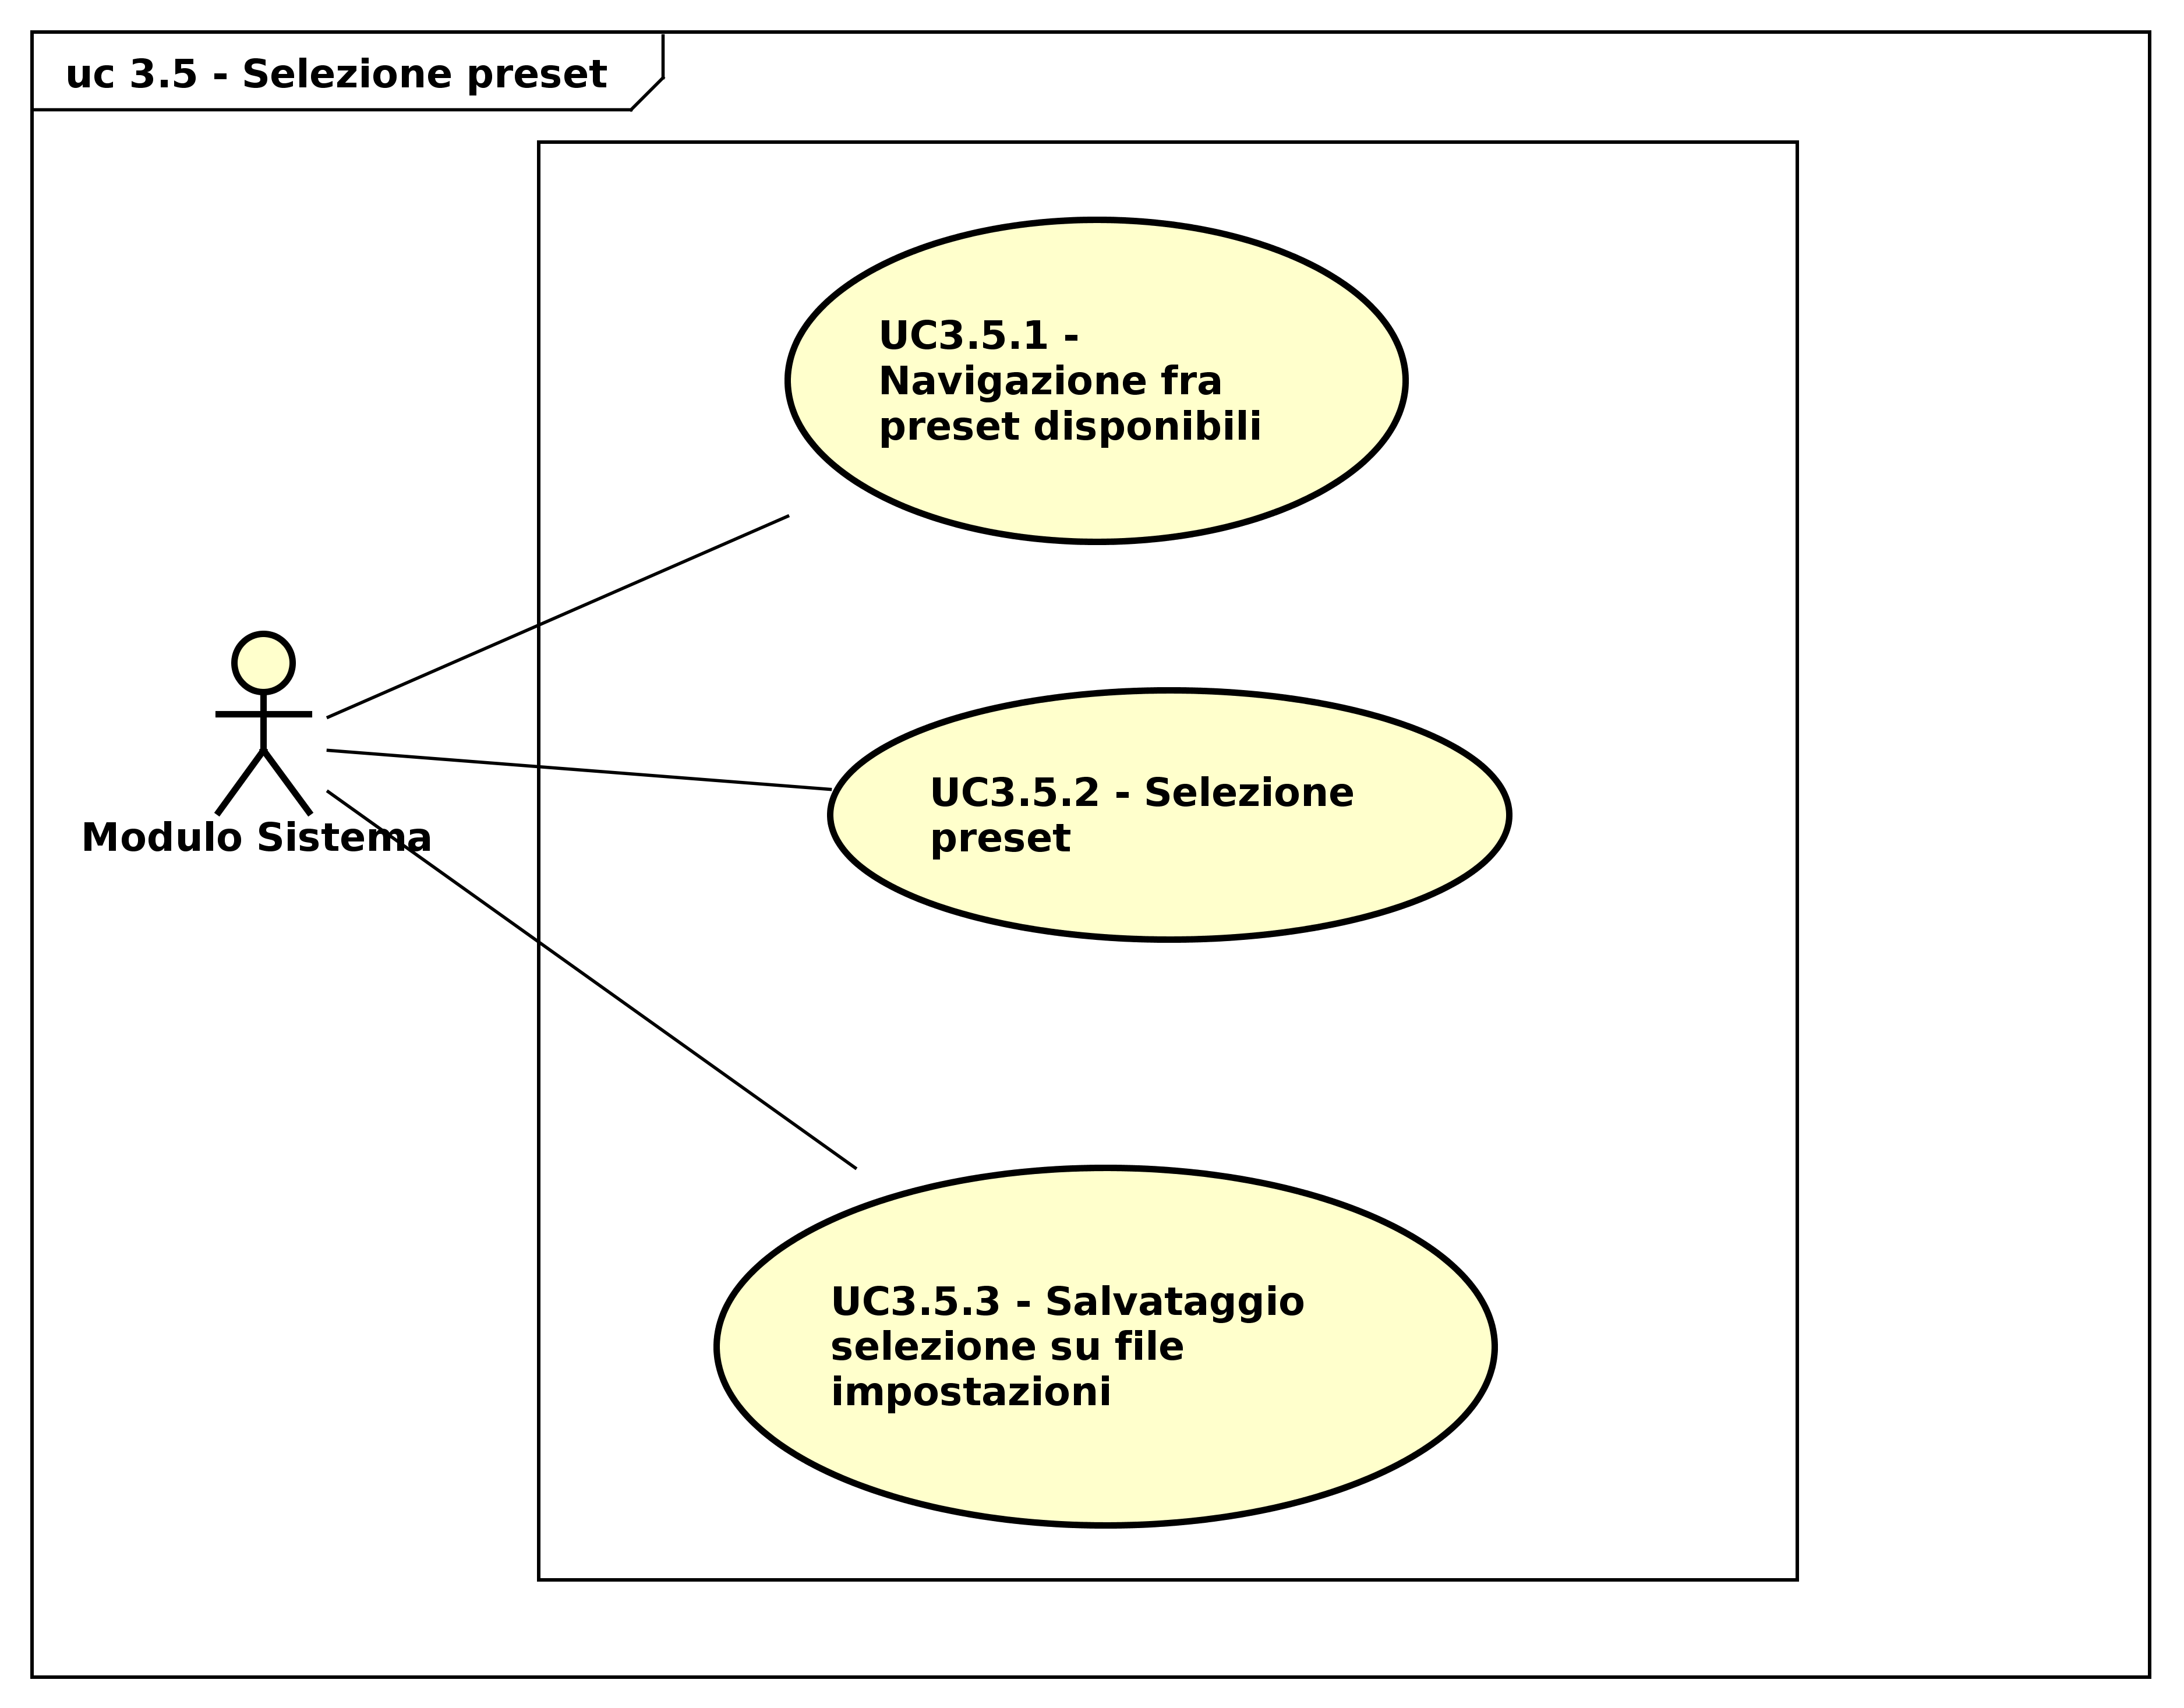
\includegraphics[scale=0.5]{immagini/uc3_5_selezione_preset.png}
%\captionsetup{labelfont=bf}
%\caption{Caso d'uso UC3.5}
%\end{figure}
%\newpage

\subsection{Caso d'uso UC3.6: Traduzione SSML}
\label{sec:UC3.6}

\begin{itemize}
\item \textbf{Attori}: modulo di sistema;
\item \textbf{Scopo e descrizione}: il modulo di sistema converte il testo delle battute inserite dall'utente nello sceneggiato in SSML\G;
\item \textbf{Precondizione}: il modulo ha ricevuto correttamente il testo inserito dall'utente;
\item \textbf{Flusso principale degli eventi}:
\begin{enumerate}
\item Il modulo esegue l'\textit{encoding}\G\ e l'\textit{escaping}\G\ del testo (UC3.6.1);
\item Il modulo crea i \textit{tag}\G\ conformi al linguaggio SSML (UC3.6.2);
\item Il modulo inserisce i parametri e gli attributi nei \textit{tag} (UC3.6.3).
\end{enumerate}
\item \textbf{Postcondizione}: il testo è stato convertito correttamente seguendo le regole del linguaggio SSML.
\end{itemize}
\begin{figure}[htbp]
\centering
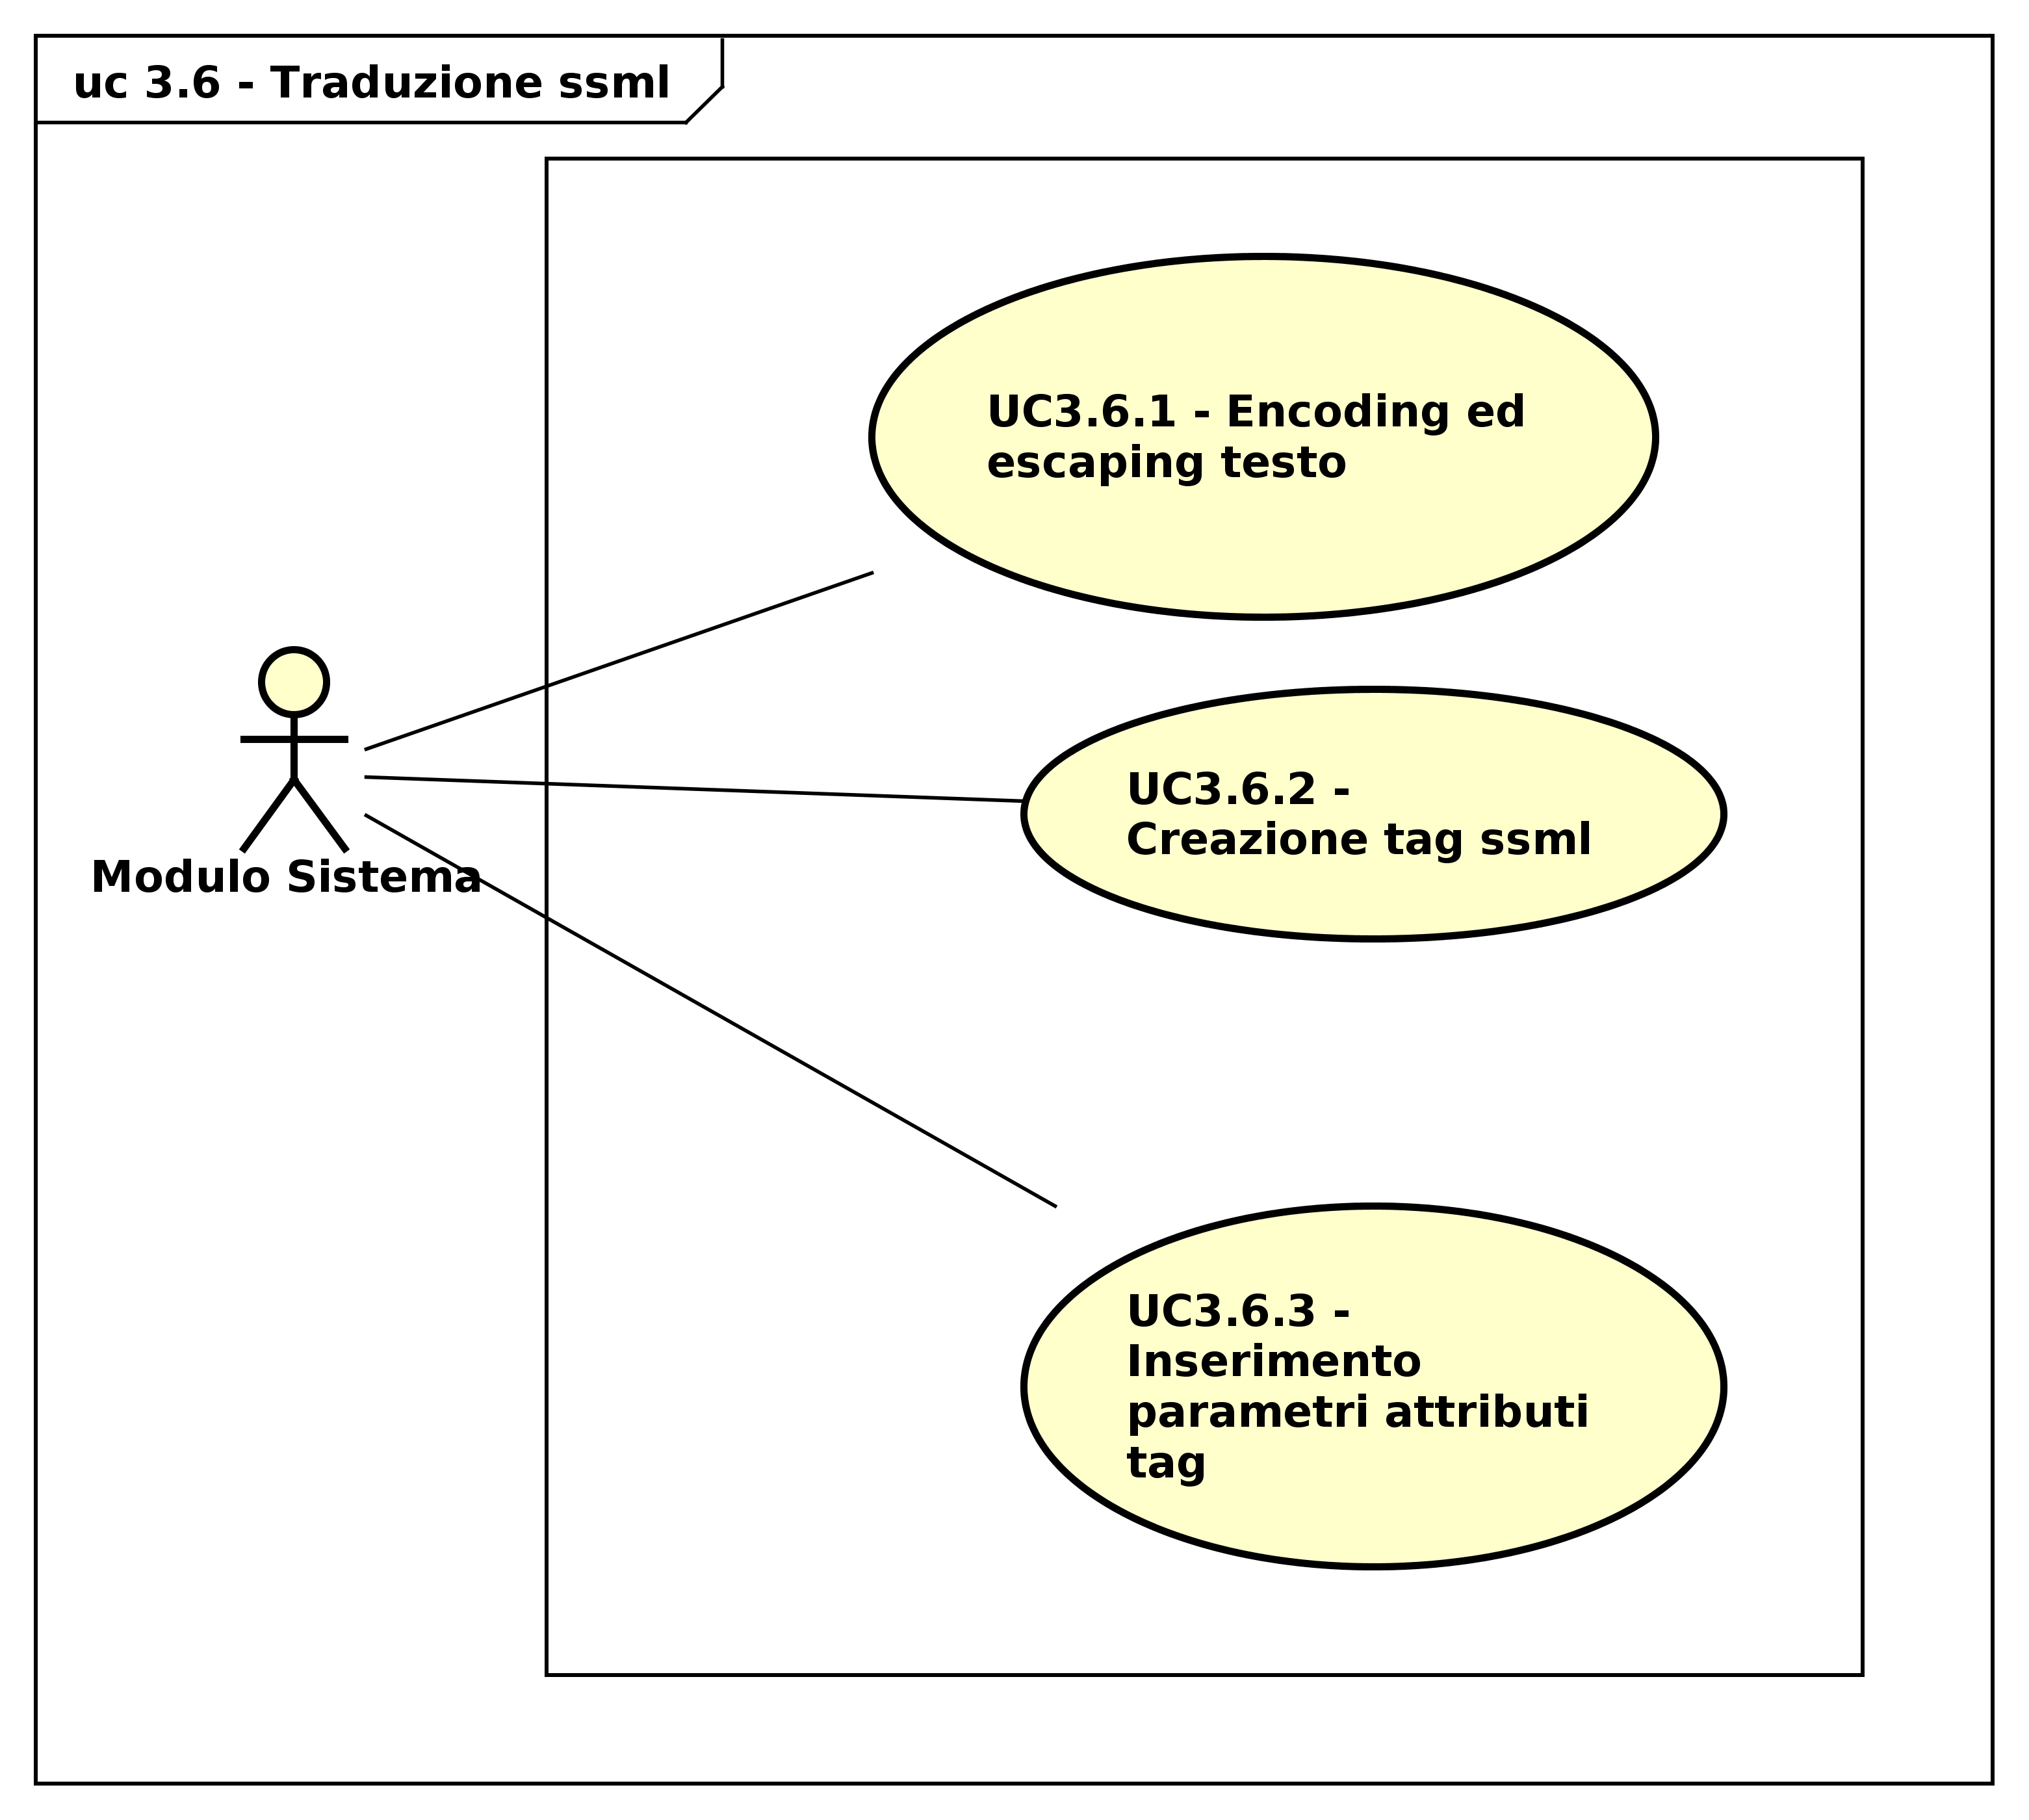
\includegraphics[scale=0.5]{immagini/uc3_6_traduzione_ssml.png}
\captionsetup{labelfont=bf}
\caption{Caso d'uso UC3.5}
\end{figure}
\newpage
\section{Requisiti}
Di seguito si riportano tutti i requisiti individuati, che derivano da casi d’uso, dal capitolato, dai \textit{meeting} con il Proponente e dalle esigenze del gruppo \GRUPPO. Sono divisi in tabelle separate a seconda della loro categoria. Di ogni requisito si specificano la tipologia, la priorità, la descrizione e ne viene indicata la provenienza.
I requisiti prodotti devono essere classificati a seconda del tipo e dell'importanza, rispettando la seguente notazione:

\begin{center}
	R[Importanza][Tipo][Codice]
\end{center}

\begin{itemize}
	\item\textbf{Importanza}: i valori che può assumere sono:
	
	\begin{itemize}
		\item[-] 0: requisito obbligatorio;
		\item[-] 1: requisito desiderabile;
		\item[-] 2: requisito opzionale.
	\end{itemize}
	
	\item\textbf{Tipo}: i valori che può assumere sono:
		\begin{itemize}
			\item[-] F: requisito funzionale;
			\item[-] P: requisito prestazionale;
			\item[-] Q: requisito di qualità;
			\item[-] V: requisito di vincolo.
		\end{itemize}
	
	\item\textbf{Codice}: è il codice gerarchico e univoco del vincolo espresso nella forma X.Y.Z dove X, Y e Z sono dei valori numerici.
\end{itemize}
Inoltre, ogni requisito deve contenere le seguenti informazioni:
	
\begin{itemize}
	\item\textbf{Descrizione}: descrizione del requisito con la minore ambiguità possibile;
	\item\textbf{Fonte}: la scelta può ricadere tra:
	\begin{itemize}
		\item[-] \textbf{Capitolato}: requisito ottenuto dalle specifiche del capitolato;
		\item[-] \textbf{Interno}: requisito elaborato dagli \textit{Analisti} nel corso di un'analisi più approfondita del problema;
		\item[-] \textbf{Caso d'uso}: requisito ottenuto da uno o più casi d'uso. Deve essere quindi specificato il codice del caso d'uso a cui ci si riferisce;
		\item[-] \textbf{Verbale}: requisito ottenuto da un incontro con il Proponente o da riunioni interne tra i membri del gruppo di lavoro \GRUPPO.
	\end{itemize}
\end{itemize}

\newpage

\subsection{Requisiti funzionali}
\begin{center}
\def\arraystretch{1.6}
\bgroup
\begin{longtable}{| p{2.5cm} | p{3cm} | p{5.25cm} | p{2cm} |}
\hline
\textbf{Requisito} & \textbf{Tipologia} & \textbf{Descrizione} & \textbf{Fonti}\\ \hline \hline  R0F1 & Funzionale \newline Obbligatorio & Il programma deve permettere la creazione di sceneggiati &  \hyperref[sec:UC1.1]{ UC1.1 }  \\ \hline  R0F1.1 & Funzionale \newline Obbligatorio & L'utente deve poter assegnare un titolo allo sceneggiato &  \hyperref[sec:UC1.1.6]{ UC1.1.6 }  \\ \hline  R0F1.1.1 & Funzionale \newline Obbligatorio & L'utente deve poter modificare il titolo ad uno sceneggiato &  \hyperref[sec:UC1.1.6]{ UC1.1.6 } \newline \hyperref[sec:UC1.8]{ UC1.8 }  \\ \hline  R0F1.2 & Funzionale \newline Obbligatorio & L'utente deve poter creare un nuovo personaggio per lo sceneggiato &  \hyperref[sec:UC1.1.1]{ UC1.1.1 }  \\ \hline  R0F1.2.1 & Funzionale \newline Obbligatorio & L'utente deve poter assegnare un nome al personaggio creato &  \hyperref[sec:UC1.1.1.1]{ UC1.1.1.1 }  \\ \hline  R0F1.2.1.1 & Funzionale \newline Obbligatorio & L'utente deve poter modificare il nome associato ad un personaggio &  \hyperref[sec:UC1.1.1.1]{ UC1.1.1.1 }  \\ \hline  R0F1.2.2 & Funzionale \newline Obbligatorio & L'utente deve poter assegnare un \textit{avatar}\G\ al personaggio creato &  \hyperref[sec:UC1.1.1.3]{ UC1.1.1.3 }  \\ \hline  R0F1.2.2.1 & Funzionale \newline Obbligatorio & L'utente deve poter aprire un'immagine &  \hyperref[sec:UC1.1.1.3]{ UC1.1.1.3 } \newline \hyperref[sec:UC1.7.1]{ UC1.7.1 }  \\ \hline  R1F1.2.2.1.1 & Funzionale \newline Desiderabile & L'utente deve poter navigare nel \textit{filesystem}\G\ per aprire un'immagine &  \hyperref[sec:UC1.7.1]{ UC1.7.1 }  \\ \hline  R1F1.2.3 & Funzionale \newline Desiderabile & L'utente deve poter cambiare l'\textit{avatar}\G\ al personaggio creato &  \hyperref[sec:UC1.1.1.3]{ UC1.1.1.3 }  \\ \hline  R0F1.2.4 & Funzionale \newline Obbligatorio & L'utente deve poter assegnare una voce al personaggio creato &  \hyperref[sec:UC1.1.1.2]{ UC1.1.1.2 } \newline \hyperref[sec:UC1.1.1.2.2]{ UC1.1.1.2.2 }  \\ \hline  R0F1.2.4.1 & Funzionale \newline Obbligatorio & L'utente deve poter visualizzare le voci disponibili  &  \hyperref[sec:UC1.1.1.2.1]{ UC1.1.1.2.1 }  \\ \hline  R0F1.2.5 & Funzionale \newline Obbligatorio & L'utente deve poter modificare la voce di un personaggio &  \hyperref[sec:UC1.1.1.2.2]{ UC1.1.1.2.2 }  \\ \hline  R0F1.2.5.1 & Funzionale \newline Obbligatorio & L'utente deve poter modificare i parametri che definiscono una voce &  \hyperref[sec:UC1.1.1.5]{ UC1.1.1.5 }  \\ \hline  R0F1.2.5.1.1 & Funzionale \newline Obbligatorio & L'utente deve poter modificare il nome associato ad una voce &  \hyperref[sec:UC1.1.1.5]{ UC1.1.1.5 }  \\ \hline  R0F1.2.6 & Funzionale \newline Obbligatorio & L'utente deve poter scrivere una battuta &  \hyperref[sec:UC1.1.2.3]{ UC1.1.2.3 }  \\ \hline  R0F1.2.6.1 & Funzionale \newline Obbligatorio & L'utente deve poter associare un personaggio ad ogni battuta &  \hyperref[sec:UC1.1.2.3.1]{ UC1.1.2.3.1 } \newline \hyperref[sec:UC1.1.2.3.2]{ UC1.1.2.3.2 }  \\ \hline  R0F1.2.6.2 & Funzionale \newline Obbligatorio & L'utente deve poter modificare il personaggio associato ad una battuta &  \hyperref[sec:UC1.1.1]{ UC1.1.1 }  \\ \hline  R0F1.2.6.3 & Funzionale \newline Obbligatorio & L'utente deve poter cancellare una battuta &  \hyperref[sec:UC1.1.2.5]{ UC1.1.2.5 }  \\ \hline  R0F1.2.6.4 & Funzionale \newline Obbligatorio & L'utente deve poter associare un sentimento ad ogni battuta  &  \hyperref[sec:UC1.1.2.6]{ UC1.1.2.6 }  \\ \hline  R0F1.2.6.4.1 & Funzionale \newline Obbligatorio & L'utente deve poter visualizzare i sentimenti disponibili &  \hyperref[sec:UC1.1.3.2]{ UC1.1.3.2 }  \\ \hline  R0F1.2.6.5 & Funzionale \newline Obbligatorio & L'utente deve poter modificare il sentimento associato ad una battuta &  \hyperref[sec:UC1.1.2.4.3]{ UC1.1.2.4.3 }  \\ \hline  R0F1.2.6.6 & Funzionale \newline Obbligatorio & L'utente deve poter cambiare il personaggio associato ad ogni battuta &  \hyperref[sec:UC1.1.2.4.4]{ UC1.1.2.4.4 }  \\ \hline  R0F1.2.6.7 & Funzionale \newline Obbligatorio & L'utente deve poter modificare il testo di ogni battuta &  \hyperref[sec:UC1.1.2.4.2]{ UC1.1.2.4.2 }  \\ \hline  R2F1.2.6.8 & Funzionale \newline Opzionale & L'utente deve poter ascoltare ogni battuta singolarmente &  \hyperref[sec:UC1.1.2.6.2]{ UC1.1.2.6.2 }  \\ \hline  R0F1.2.6.9 & Funzionale \newline Obbligatorio & L'utente deve poter selezionare una battuta &  \hyperref[sec:UC1.2.4.1]{ UC1.2.4.1 }  \\ \hline  R0F1.2.7 & Funzionale \newline Obbligatorio & L'utente deve poter visualizzare l'elenco dei personaggi a disposizione &  \hyperref[sec:UC1.1.2.3.1]{ UC1.1.2.3.1 }  \\ \hline  R0F1.2.8 & Funzionale \newline Obbligatorio & L'utente deve poter creare una nuova voce &  \hyperref[sec:UC1.1.1.4]{ UC1.1.1.4 }  \\ \hline  R0F1.2.8.1 & Funzionale \newline Obbligatorio & Al momento della creazione di una nuova voce, l'utente deve poter selezionare la lingua &  \hyperref[sec:UC1.1.1.4.1]{ UC1.1.1.4.1 }  \\ \hline  R0F1.2.8.2 & Funzionale \newline Obbligatorio & Al momento della creazione di una nuova voce, l'utente deve poter selezionare il sesso &  \hyperref[sec:UC1.1.1.4.2]{ UC1.1.1.4.2 }  \\ \hline  R0F1.2.8.3 & Funzionale \newline Obbligatorio & Al momento della creazione di una nuova voce, l'utente può modificare i parametri di una voce &  \hyperref[sec:UC1.1.1.4.3]{ UC1.1.1.4.3 }  \\ \hline  R0F1.2.8.4 & Funzionale \newline Obbligatorio & Al momento della creazione di una nuova voce, l'utente deve poter assegnare un nome alla stessa &  \hyperref[sec:Capitolato]{ Capitolato } \newline \hyperref[sec:UC1.1.1.4.4]{ UC1.1.1.4.4 }  \\ \hline  R0F1.3 & Funzionale \newline Obbligatorio & L'utente deve poter cancellare un personaggio &  \hyperref[sec:UC1.1.1]{ UC1.1.1 }  \\ \hline  R1F1.4 & Funzionale \newline Desiderabile & L'utente deve poter condividere l'audio dello sceneggiato &  \hyperref[sec:UC1.10]{ UC1.10 }  \\ \hline  R1F1.4.1 & Funzionale \newline Desiderabile & L'utente deve poter navigare fra le opzioni di condivisione &  \hyperref[sec:UC1.2.1]{ UC1.2.1 }  \\ \hline  R1F1.4.2 & Funzionale \newline Desiderabile & L'applicazione deve reperire gli strumenti di condivisione disponibili nel sistema &  \hyperref[sec:UC1.2.3]{ UC1.2.3 }  \\ \hline  R1F1.4.3 & Funzionale \newline Desiderabile & L'utente deve poter selezionare lo strumento di condivisione che preferisce &  \hyperref[sec:UC1.2.2]{ UC1.2.2 }  \\ \hline  R0F1.6 & Funzionale \newline Obbligatorio & L'utente deve poter esportare lo sceneggiato in un \textit{file} audio &  \hyperref[sec:UC1.3]{ UC1.3 }  \\ \hline  R1F1.6.1 & Funzionale \newline Desiderabile & L'utente deve poter selezionare il formato audio di esportazione &  \hyperref[sec:UC1.3.1]{ UC1.3.1 }  \\ \hline  R0F1.6.1.2 & Funzionale \newline Obbligatorio & Deve essere possibile esportare lo sceneggiato nel formato wav\G\ &  \hyperref[sec:UC1.3]{ UC1.3 }  \\ \hline  R0F1.6.2 & Funzionale \newline Obbligatorio & L'utente deve poter indicare il nome di salvataggio del \textit{file} audio &  \hyperref[sec:UC1.3.2]{ UC1.3.2 }  \\ \hline  R0F1.7 & Funzionale \newline Obbligatorio & L'utente deve poter salvare lo sceneggiato &  \hyperref[sec:UC1.5]{ UC1.5 }  \\ \hline  R0F1.7.1 & Funzionale \newline Obbligatorio & L'utente deve poter scegliere con che nome salvare lo sceneggiato &  \hyperref[sec:UC1.5]{ UC1.5 }  \\ \hline  R2F1.7.3 & Funzionale \newline Opzionale & L'utente deve poter salvare il \textit{file} video esportato &  \hyperref[sec:UC1.13]{ UC1.13 }  \\ \hline  R1F1.8.3 & Funzionale \newline Desiderabile & All'avvio dell'applicazione deve essere aperto l'ultimo sceneggiato creato &  \hyperref[sec:UC1.9]{ UC1.9 }  \\ \hline  R0F1.9 & Funzionale \newline Obbligatorio & L'utente deve poter aprire uno sceneggiato salvato in precedenza &  \hyperref[sec:UC1.7.2]{ UC1.7.2 }  \\ \hline  R0F1.9.1 & Funzionale \newline Obbligatorio & Deve essere disponibile una lista contenente tutti gli sceneggiati salvati  &  \hyperref[sec:UC1.7]{ UC1.7 }  \\ \hline  R1F1.10 & Funzionale \newline Desiderabile & L'utente deve poter ascoltare una parte selezionata dello sceneggiato &  \hyperref[sec:UC1.1.2.7]{ UC1.1.2.7 } \newline \hyperref[sec:UC1.8.2]{ UC1.8.2 }  \\ \hline  R0F1.11 & Funzionale \newline Obbligatorio & L'utente può creare un nuovo capitolo &  \hyperref[sec:UC1.1.2]{ UC1.1.2 }  \\ \hline  R0F1.11.1 & Funzionale \newline Obbligatorio & L'utente deve poter modificare un capitolo &  \hyperref[sec:UC1.8.1]{ UC1.8.1 }  \\ \hline  R0F1.11.1.2 & Funzionale \newline Obbligatorio & L'utente deve poter modificare il titolo di un capitolo &  \hyperref[sec:UC1.8.1.4]{ UC1.8.1.4 }  \\ \hline  R1F1.11.1.4 & Funzionale \newline Desiderabile & L'utente deve poter modificare lo sfondo assegnato ad un capitolo &  \hyperref[sec:UC1.8.1.3]{ UC1.8.1.3 }  \\ \hline  R1F1.11.1.8 & Funzionale \newline Desiderabile & L'utente deve poter modificare l'immagine di sfondo &  \hyperref[sec:UC1.8.1.3]{ UC1.8.1.3 }  \\ \hline  R2F1.11.1.9 & Funzionale \newline Opzionale & L'utente deve poter modificare la traccia audio di sfondo di un capitolo &  \hyperref[sec:UC1.8.1.3]{ UC1.8.1.3 }  \\ \hline  R0F1.11.1.11 & Funzionale \newline Obbligatorio & L'utente deve poter selezionare un singolo capitolo &  \hyperref[sec:UC1.8.1.1]{ UC1.8.1.1 }  \\ \hline  R0F1.11.2 & Funzionale \newline Obbligatorio & L'utente deve poter assegnare un titolo al capitolo &  \hyperref[sec:UC1.1.2.1]{ UC1.1.2.1 }  \\ \hline  R1F1.11.3 & Funzionale \newline Desiderabile & L'utente deve avere a disposizione un'anteprima del capitolo &  \hyperref[sec:UC1.8.1.2]{ UC1.8.1.2 }  \\ \hline  R1F1.11.4 & Funzionale \newline Desiderabile & L'utente deve poter inserire uno sfondo da associare ad un capitolo &  \hyperref[sec:UC1.1.2.2]{ UC1.1.2.2 }  \\ \hline  R1F1.11.4.1 & Funzionale \newline Desiderabile & L'utente deve poter caricare un'immagine di sfondo &  \hyperref[sec:UC1.1.2.2.1]{ UC1.1.2.2.1 }  \\ \hline  R1F1.11.4.2 & Funzionale \newline Desiderabile & L'utente deve poter inserire un sottofondo sonoro &  \hyperref[sec:UC1.1.2.2.2]{ UC1.1.2.2.2 }  \\ \hline  R1F1.11.5 & Funzionale \newline Desiderabile & L'utente deve poter inserire un suono tra le battute &  \hyperref[sec:UC1.1.2.8]{ UC1.1.2.8 }  \\ \hline  R2F1.11.6 & Funzionale \newline Opzionale & L'utente deve poter caricare un suono da inserire tra le battute &  \hyperref[sec:UC1.1.2.8]{ UC1.1.2.8 }  \\ \hline  R0F1.11.7 & Funzionale \newline Obbligatorio & L'utente deve poter togliere un suono precedentemente inserito &  \hyperref[sec:UC1.8.1.5]{ UC1.8.1.5 }  \\ \hline  R1F1.12 & Funzionale \newline Desiderabile & L'utente deve poter esportare lo sceneggiato in un video &  \hyperref[sec:UC1.4]{ UC1.4 }  \\ \hline  R2F1.12.1 & Funzionale \newline Opzionale & L'utente deve poter scegliere il formato video di esportazione &  \hyperref[sec:UC1.3.1]{ UC1.3.1 }  \\ \hline  R1F1.13 & Funzionale \newline Desiderabile & L'utente deve poter cambiare l'ordine dei capitoli &  \hyperref[sec:UC1.1.4]{ UC1.1.4 }  \\ \hline  R0F2 & Funzionale \newline Obbligatorio & L'utente deve poter creare delle configurazioni di effetti personali &  \hyperref[sec:UC2.1]{ UC2.1 }  \\ \hline  R0F2.1 & Funzionale \newline Obbligatorio & L'utente deve poter navigare fra le configurazioni di effetti disponibili &  \hyperref[sec:UC2.1.1]{ UC2.1.1 }  \\ \hline  R0F2.2 & Funzionale \newline Obbligatorio & Il modulo di sistema deve reperire gli effetti disponibili &  \hyperref[sec:UC3.2]{ UC3.2 }  \\ \hline  R0F2.3 & Funzionale \newline Obbligatorio & L'utente deve poter impostare i parametri di ogni configurazione di effetti &  \hyperref[sec:UC2.1.2]{ UC2.1.2 }  \\ \hline  R0F2.4 & Funzionale \newline Obbligatorio & L'utente deve poter testare le configurazioni di effetti ascoltando la sintesi di un testo di prova &  \hyperref[sec:UC2.4]{ UC2.4 }  \\ \hline  R0F2.5 & Funzionale \newline Obbligatorio & L'utente deve poter modificare i parametri di una configurazione di effetti &  \hyperref[sec:UC2.5]{ UC2.5 }  \\ \hline  R0F3 & Funzionale \newline Obbligatorio & L'utente deve poter salvare le configurazioni di effetti create &  \hyperref[sec:UC2.1]{ UC2.1 }  \\ \hline  R0F3.1 & Funzionale \newline Obbligatorio & L'utente deve poter decidere il nome con cui salvare una configurazione di effetti &  \hyperref[sec:UC2.1.3]{ UC2.1.3 }  \\ \hline  R2F4 & Funzionale \newline Opzionale & L'utente deve poter selezionare una voce per personalizzare il servizio TTS\G\ di sistema &  \hyperref[sec:UC2.2]{ UC2.2 }  \\ \hline  R0F4.1 & Funzionale \newline Obbligatorio & L'utente deve poter navigare fra le voci di sistema disponibili &  \hyperref[sec:UC2.2]{ UC2.2 } \newline \hyperref[sec:UC2.2.1]{ UC2.2.1 }  \\ \hline  R0F5 & Funzionale \newline Obbligatorio & Il modulo di sistema deve poter reperire le voci disponibili nel sistema &  \hyperref[sec:UC3.1]{ UC3.1 }  \\ \hline  R0F6 & Funzionale \newline Obbligatorio & Il modulo di sistema deve poter reperire le voci offerte dal server di \AZIENDA &  \hyperref[sec:UC3.1]{ UC3.1 }  \\ \hline  R0F7 & Funzionale \newline Obbligatorio & Il modulo di sistema deve poter comunicare con il server di \AZIENDA &  \hyperref[sec:UC3.3]{ UC3.3 }  \\ \hline  R0F7.1 & Funzionale \newline Obbligatorio & Il modulo di sistema deve essere in grado di creare una corretta richiesta HTTP\G &  \hyperref[sec:UC3.3.1]{ UC3.3.1 }  \\ \hline  R0F7.2 & Funzionale \newline Obbligatorio & Il modulo di sistema deve essere in grado di ricevere le risposte delle richieste effettuate dal server di \AZIENDA &  \hyperref[sec:UC3.3.3]{ UC3.3.3 }  \\ \hline  R0F9 & Funzionale \newline Obbligatorio & Il modulo di sistema deve ottenere dal server di \AZIENDA\ la lista degli effetti disponibili &  \hyperref[sec:UC3.2]{ UC3.2 }  \\ \hline  R0F10 & Funzionale \newline Obbligatorio & Il modulo di sistema deve essere in grado di formulare una richiesta HTTP\G\ per la ricezione degli effetti &  \hyperref[sec:UC3.2]{ UC3.2 }  \\ \hline  R1F12 & Funzionale \newline Desiderabile & Il modulo di sistema deve integrarsi con il servizio TTS\G\ del sistema, per mettere a disposizione nuove voci alle applicazioni installate &  \hyperref[sec:Capitolato]{ Capitolato }  \\ \hline  R1F14 & Funzionale \newline Desiderabile & Il modulo di sistema deve poter convertire una battuta in SSML\G  &  \hyperref[sec:UC1.1.2.3.4]{ UC1.1.2.3.4 }  \\ \hline  R1F15 & Funzionale \newline Desiderabile & L'utente deve poter condividere un video &  \hyperref[sec:UC1.11]{ UC1.11 }  \\ \hline  R1F15.1 & Funzionale \newline Desiderabile & L'utente deve poter scegliere se condividere audio o video &  \hyperref[sec:UC1.2.4]{ UC1.2.4 }  \\ \hline  R0F16 & Funzionale \newline Obbligatorio & L'utente deve poter modificare uno sceneggiato già creato &  \hyperref[sec:UC1.8]{ UC1.8 }  \\ \hline  R1F16.2 & Funzionale \newline Desiderabile & L'applicazione deve fornire un'anteprima dello sceneggiato su richiesta dell'utente &  \hyperref[sec:UC1.8.2]{ UC1.8.2 }  \\ \hline  R2F17 & Funzionale \newline Opzionale & L'utente deve avere la possibilità di campionare la propria voce &  \hyperref[sec:UC2.3]{ UC2.3 }  \\ \hline  R2F17.1 & Funzionale \newline Opzionale & L'utente deve poter effettuare la \textit{login}\G\ al sito di \AZIENDA &  \hyperref[sec:UC2.3.4]{ UC2.3.4 }  \\ \hline  R2F17.2 & Funzionale \newline Opzionale & L'utente deve poter visualizzare le frasi da leggere nella fase di campionamento &  \hyperref[sec:UC2.3.1]{ UC2.3.1 }  \\ \hline  R2F17.3 & Funzionale \newline Opzionale & L'utente deve potersi registrare durante la lettura delle frasi necessaria per il campionamento &  \hyperref[sec:UC2.3.2]{ UC2.3.2 }  \\ \hline  R2F17.4 & Funzionale \newline Opzionale & L'applicazione deve essere in grado di inviare al server di \AZIENDA\ le registrazioni necessarie per il campionamento &  \hyperref[sec:UC2.3.3]{ UC2.3.3 }  \\ \hline  R2F17.5 & Funzionale \newline Opzionale & L'utente deve poter interrompere il processo di campionamento senza perdere i dati già salvati &  \hyperref[sec:UC2.3]{ UC2.3 }  \\ \hline  R2F17.6 & Funzionale \newline Opzionale & L'utente deve poter riprendere il processo di campionamento in qualsiasi momento  &  \hyperref[sec:UC2.3]{ UC2.3 }  \\ \hline  R2F18 & Funzionale \newline Opzionale & L'utente deve potersi registrare al sito di \AZIENDA &  \hyperref[sec:UC2.3]{ UC2.3 }  \\ \hline  R0F19 & Funzionale \newline Obbligatorio & L'utente deve poter aprire un audio &  \hyperref[sec:UC1.7]{ UC1.7 }  \\ \hline  R0F19.1 & Funzionale \newline Obbligatorio & L'utente deve poter navigare nel \textit{filesystem}\G\ per aprire un file audio &  \hyperref[sec:UC1.7.0.1]{ UC1.7.0.1 }  \\ \hline \caption{Requisiti funzionali}
\end{longtable}
\egroup
\end{center} \newpage \subsection{Requisiti qualitativi}
\begin{center}
\def\arraystretch{1.6}
\bgroup
\begin{longtable}{| p{2.5cm} | p{3cm} | p{5.25cm} | p{2cm} |}
\hline
\textbf{Requisito} & \textbf{Tipologia} & \textbf{Descrizione} & \textbf{Fonti}\\ \hline \hline  R0Q1.5 & Di qualità \newline Obbligatorio & Devono essere offerti meccanismi di annullamento delle operazioni svolte dall'utente &  \hyperref[sec:Accessibilità ]{ Accessibilità  }  \\ \hline  R1Q1.6.3 & Di qualità \newline Desiderabile & Nel caso la condivisione fallisse deve essere fornita come opzione all'utente l'esportazione e il salvataggio in locale del \textit{file} audio &  \hyperref[sec:UC1.2]{ UC1.2 } \newline \hyperref[sec:UC1.3]{ UC1.3 }  \\ \hline  R1Q1.7.2 & Di qualità  \newline Desiderabile & Nel caso il salvataggio non andasse a buon fine deve essere fornito all'utente un messaggio di errore &  \hyperref[sec:UC1.5]{ UC1.5 } \newline \hyperref[sec:UC1.5.3]{ UC1.5.3 }  \\ \hline  R1Q1.8 & Di qualità  \newline Desiderabile & Il sistema deve effettuare salvataggi automatici ogni minuto &  \hyperref[sec:UC1.9]{ UC1.9 }  \\ \hline  R1Q1.8.2 & Di qualità \newline Desiderabile & Deve essere possibile recuperare la sessione corrente in caso di \textit{crash}\G\ del programma &  \hyperref[sec:UC1.9]{ UC1.9 }  \\ \hline  R1Q7.3 & Di qualità  \newline Desiderabile & In caso di connessione assente l'utente deve poter visualizzare un opportuno messaggio di errore &  \hyperref[sec:UC3.3.4]{ UC3.3.4 }  \\ \hline  R1Q7.4 & Di qualità  \newline Desiderabile & In caso la connessione venisse meno a processo avviato, l'utente deve poter visualizzare un opportuno messaggio di errore &  \hyperref[sec:UC3.3]{ UC3.3 } \newline \hyperref[sec:UC3.3.4]{ UC3.3.4 }  \\ \hline  R2Q8 & Di qualità  \newline Opzionale & In caso di assenza di connessione l'utente deve poter utilizzare l'applicazione con le voci di sistema &  \hyperref[sec:Capitolato]{ Capitolato }  \\ \hline  R1Q11 & Di qualità  \newline Desiderabile & Il modulo di sistema deve essere in grado di mantenere nella memoria l'audio ricevuto dal server \AZIENDA  &  \hyperref[sec:UC3.4]{ UC3.4 }  \\ \hline  R1Q20 & Di qualità  \newline Desiderabile & L'applicazione deve utilizzare meccanismi di \textit{caching}\G\ per ridurre il tempo di attesa dovuto alla connessione &  \hyperref[sec:Capitolato]{ Capitolato }  \\ \hline  R0Q22 & Di qualità \newline Obbligatorio & La conversione in mp3\G\ avviene solo dopo l'assemblamento di tutte le parti in formato wav\G\ &  \hyperref[sec:Capitolato]{ Capitolato }  \\ \hline  R1Q23 & Di qualità \newline Desiderabile & Deve essere garantita l'esportazione in mp3\G\ per risparmiare spazio nel dispositivo  &  \\ \hline \caption{Requisiti di qualità}
\end{longtable}
\egroup
\end{center} \newpage \subsection{Requisiti prestazionali}
\begin{center}
\def\arraystretch{1.6}
\bgroup
\begin{longtable}{| p{2.5cm} | p{3cm} | p{5.25cm} | p{2cm} |}
\hline
\textbf{Requisito} & \textbf{Tipologia} & \textbf{Descrizione} & \textbf{Fonti}\\ \hline \hline  R0P20.1 & Prestazionale \newline Obbligatorio & Ogni volta che una battuta viene creata o modificata il modulo di sistema deve richiedere l'audio al server e salvarlo nella memoria locale  &  \hyperref[sec:Capitolato]{ Capitolato }  \\ \hline \caption{Requisiti prestazionali}
\end{longtable}
\egroup
\end{center} \newpage \subsection{Vincoli}
\begin{center}
\def\arraystretch{1.6}
\bgroup
\begin{longtable}{| p{2.5cm} | p{3cm} | p{5.25cm} | p{2cm} |}
\hline
\textbf{Requisito} & \textbf{Tipologia} & \textbf{Descrizione} & \textbf{Fonti}\\ \hline \hline  R1V1.6.1.1 & Vincolo \newline Desiderabile & Deve essere possibile esportare nel formato mp3\G\ &  \hyperref[sec:UC1.3]{ UC1.3 }  \\ \hline  R0V1.8.1 & Vincolo \newline Obbligatorio & L'applicazione deve salvare i \textit{file} in una cartella di default &  \hyperref[sec:UC1.12]{ UC1.12 }  \\ \hline  R0V13 & Vincolo \newline Obbligatorio & Il modulo di sistema deve integrarsi con il sistema Android\G &  \hyperref[sec:Capitolato]{ Capitolato }  \\ \hline  R0V21 & Vincolo \newline Obbligatorio & Il modulo di sistema deve utilizzare il linguaggio SSML\G &  \hyperref[sec:Verbale 18/03/2016]{ Verbale 18/03/2016 }  \\ \hline  R1V24 & Vincolo \newline Desiderabile & Il sistema deve essere compatibile con versioni di Android\G\ a partire dalla 4.0 &  \\ \hline  R0V25 & Vincolo \newline Obbligatorio & Il progetto deve essere pubblicato su GitHub\G &  \\ \hline  R0V26 & Vincolo \newline Obbligatorio & Il sistema deve permettere l’interrogazione alle API\G\ di \AZIENDA &  \\ \hline \caption{Vincoli}
\end{longtable}
\egroup
\end{center} \newpage \subsection{Tracciamento Fonti-Requisiti}
\begin{center}
\def\arraystretch{1.6}
\bgroup
\begin{longtable}{| p{10.25cm} | p{2.5cm} | }
\hline
\textbf{Fonte} & \textbf{Requisito} \\ \hline \hline  \hyperref[sec:Accessibilità ]{ Accessibilità   } &  R0Q1.5  \\ \hline  \hyperref[sec:Capitolato]{ Capitolato  } &  R2Q8  \newline R1F12  \newline R0V13  \newline R0F1.2.8.4  \newline R1Q20  \newline R0P20.1  \newline R0Q22  \\ \hline  \hyperref[sec:UC1.1]{ UC1.1 Creazione sceneggiato } &  R0F1  \\ \hline  \hyperref[sec:UC1.1.1]{ UC1.1.1 Creazione personaggio } &  R0F1.2  \newline R0F1.2.6.2  \newline R0F1.3  \\ \hline  \hyperref[sec:UC1.1.1.1]{ UC1.1.1.1 Assegnazione nome } &  R0F1.2.1  \newline R0F1.2.1.1  \\ \hline  \hyperref[sec:UC1.1.1.2]{ UC1.1.1.2 Assegnazione voce } &  R0F1.2.4  \\ \hline  \hyperref[sec:UC1.1.1.2.1]{ UC1.1.1.2.1 Navigazione fra le voci disponibili } &  R0F1.2.4.1  \\ \hline  \hyperref[sec:UC1.1.1.2.2]{ UC1.1.1.2.2 Selezione voce } &  R0F1.2.4  \newline R0F1.2.5  \\ \hline  \hyperref[sec:UC1.1.1.3]{ UC1.1.1.3 Assegnazione \textit{avatar}\G } &  R0F1.2.2  \newline R1F1.2.3  \newline R0F1.2.2.1  \\ \hline  \hyperref[sec:UC1.1.1.4]{ UC1.1.1.4 Creazione nuova voce } &  R0F1.2.8  \\ \hline  \hyperref[sec:UC1.1.1.4.1]{ UC1.1.1.4.1 Selezione lingua } &  R0F1.2.8.1  \\ \hline  \hyperref[sec:UC1.1.1.4.2]{ UC1.1.1.4.2 Selezione sesso } &  R0F1.2.8.2  \\ \hline  \hyperref[sec:UC1.1.1.4.3]{ UC1.1.1.4.3 Modifica parametri di effetti } &  R0F1.2.8.3  \\ \hline  \hyperref[sec:UC1.1.1.4.4]{ UC1.1.1.4.4 Assegnazione nome } &  R0F1.2.8.4  \\ \hline  \hyperref[sec:UC1.1.1.5]{ UC1.1.1.5 Modifica voce esistente } &  R0F1.2.5.1  \newline R0F1.2.5.1.1  \\ \hline  \hyperref[sec:UC1.1.2]{ UC1.1.2 Creazione capitolo } &  R0F1.11  \\ \hline  \hyperref[sec:UC1.1.2.1]{ UC1.1.2.1 Assegnazione titolo } &  R0F1.11.2  \\ \hline  \hyperref[sec:UC1.1.2.2]{ UC1.1.2.2 Creazione sfondo } &  R1F1.11.4  \\ \hline  \hyperref[sec:UC1.1.2.2.1]{ UC1.1.2.2.1 Caricamento immagine di sfondo } &  R1F1.11.4.1  \\ \hline  \hyperref[sec:UC1.1.2.2.2]{ UC1.1.2.2.2 Caricamento sottofondo sonoro } &  R1F1.11.4.2  \\ \hline  \hyperref[sec:UC1.1.2.3]{ UC1.1.2.3 Scrittura battute } &  R0F1.2.6  \\ \hline  \hyperref[sec:UC1.1.2.3.1]{ UC1.1.2.3.1 Navigazione tra i personaggi } &  R0F1.2.6.1  \newline R0F1.2.7  \\ \hline  \hyperref[sec:UC1.1.2.3.2]{ UC1.1.2.3.2 Scelta personaggio } &  R0F1.2.6.1  \\ \hline  \hyperref[sec:UC1.1.2.3.4]{ UC1.1.2.3.4 Conversione in SSML\G  } &  R1F14  \\ \hline  \hyperref[sec:UC1.1.2.4.2]{ UC1.1.2.4.2 Cambio testo } &  R0F1.2.6.7  \\ \hline  \hyperref[sec:UC1.1.2.4.3]{ UC1.1.2.4.3 Cambio sentimento } &  R0F1.2.6.5  \\ \hline  \hyperref[sec:UC1.1.2.4.4]{ UC1.1.2.4.4 Cambio personaggio } &  R0F1.2.6.6  \\ \hline  \hyperref[sec:UC1.1.2.5]{ UC1.1.2.5 Cancellazione battuta } &  R0F1.2.6.3  \\ \hline  \hyperref[sec:UC1.1.2.6]{ UC1.1.2.6 Associazione battuta-effetto } &  R0F1.2.6.4  \\ \hline  \hyperref[sec:UC1.1.2.6.2]{ UC1.1.2.6.2 Anteprima battuta } &  R2F1.2.6.8  \\ \hline  \hyperref[sec:UC1.1.2.7]{ UC1.1.2.7 Anteprima scena } &  R1F1.10  \\ \hline  \hyperref[sec:UC1.1.2.8]{ UC1.1.2.8 Inserimento suono } &  R1F1.11.5  \newline R2F1.11.6  \\ \hline  \hyperref[sec:UC1.1.3.2]{ UC1.1.3.2 Navigazione tra i sentimenti } &  R0F1.2.6.4.1  \\ \hline  \hyperref[sec:UC1.1.4]{ UC1.1.4 Riordinamento capitoli } &  R1F1.13  \\ \hline  \hyperref[sec:UC1.1.6]{ UC1.1.6 Assegnazione titolo } &  R0F1.1  \newline R0F1.1.1  \\ \hline  \hyperref[sec:UC1.10]{ UC1.10 Condivisione audio } &  R1F1.4  \\ \hline  \hyperref[sec:UC1.11]{ UC1.11 Condivisione video } &  R1F15  \\ \hline  \hyperref[sec:UC1.12]{ UC1.12 Salvataggio audio } &  R0V1.8.1  \\ \hline  \hyperref[sec:UC1.13]{ UC1.13 Salvataggio video  } &  R2F1.7.3  \\ \hline  \hyperref[sec:UC1.2]{ UC1.2 Condivisione } &  R1Q1.6.3  \\ \hline  \hyperref[sec:UC1.2.1]{ UC1.2.1 Navigazione tra gli strumenti di condivisione } &  R1F1.4.1  \\ \hline  \hyperref[sec:UC1.2.2]{ UC1.2.2 Selezione strumento di condivisione } &  R1F1.4.3  \\ \hline  \hyperref[sec:UC1.2.3]{ UC1.2.3 Reperimento strumenti di condivisione } &  R1F1.4.2  \\ \hline  \hyperref[sec:UC1.2.4]{ UC1.2.4 Scelta se condividere audio o video } &  R1F15.1  \\ \hline  \hyperref[sec:UC1.2.4.1]{ UC1.2.4.1 Selezione battuta } &  R0F1.2.6.9  \\ \hline  \hyperref[sec:UC1.3]{ UC1.3 Esportazione audio finale } &  R0F1.6  \newline R1V1.6.1.1  \newline R0F1.6.1.2  \newline R1Q1.6.3  \\ \hline  \hyperref[sec:UC1.3.1]{ UC1.3.1 Selezione formato } &  R1F1.6.1  \newline R2F1.12.1  \\ \hline  \hyperref[sec:UC1.3.2]{ UC1.3.2 Inserimento nome \textit{file} } &  R0F1.6.2  \\ \hline  \hyperref[sec:UC1.4]{ UC1.4 Esportazione video finale } &  R1F1.12  \\ \hline  \hyperref[sec:UC1.5]{ UC1.5 Salvataggio \textit{file} } &  R0F1.7  \newline R0F1.7.1  \newline R1Q1.7.2  \\ \hline  \hyperref[sec:UC1.5.3]{ UC1.5.3 Visualizzazione messaggio di errore } &  R1Q1.7.2  \\ \hline  \hyperref[sec:UC1.7]{ UC1.7 Apertura \textit{file} } &  R0F1.9.1  \newline R0F19  \\ \hline  \hyperref[sec:UC1.7.0.1]{ UC1.7.0.1 Navigazione \textit{filesystem}\G } &  R0F19.1  \\ \hline  \hyperref[sec:UC1.7.1]{ UC1.7.1 Apertura immagine } &  R0F1.2.2.1  \newline R1F1.2.2.1.1  \\ \hline  \hyperref[sec:UC1.7.2]{ UC1.7.2 Apertura sceneggiato } &  R0F1.9  \\ \hline  \hyperref[sec:UC1.8]{ UC1.8 Modifica sceneggiato } &  R0F1.1.1  \newline R0F16  \\ \hline  \hyperref[sec:UC1.8.1]{ UC1.8.1 Modifica capitolo } &  R0F1.11.1  \\ \hline  \hyperref[sec:UC1.8.1.1]{ UC1.8.1.1 Selezione capitolo } &  R0F1.11.1.11  \\ \hline  \hyperref[sec:UC1.8.1.2]{ UC1.8.1.2 Anteprima capitolo } &  R1F1.11.3  \\ \hline  \hyperref[sec:UC1.8.1.3]{ UC1.8.1.3 Modifica sfondo } &  R1F1.11.1.4  \newline R1F1.11.1.8  \newline R2F1.11.1.9  \\ \hline  \hyperref[sec:UC1.8.1.4]{ UC1.8.1.4 Modifica titolo capitolo } &  R0F1.11.1.2  \\ \hline  \hyperref[sec:UC1.8.1.5]{ UC1.8.1.5 Rimozione suono } &  R0F1.11.7  \\ \hline  \hyperref[sec:UC1.8.2]{ UC1.8.2 Anteprima sceneggiato } &  R1F1.10  \newline R1F16.2  \\ \hline  \hyperref[sec:UC1.9]{ UC1.9 Salvataggio di emergenza } &  R1Q1.8  \newline R1Q1.8.2  \newline R  \newline R1F1.8.3  \\ \hline  \hyperref[sec:UC2.1]{ UC2.1 Creazione \textit{preset}\G } &  R0F2  \newline R0F3  \\ \hline  \hyperref[sec:UC2.1.1]{ UC2.1.1 Navigazione tra effetti disponibili } &  R0F2.1  \\ \hline  \hyperref[sec:UC2.1.2]{ UC2.1.2 Impostazione parametri } &  R0F2.3  \\ \hline  \hyperref[sec:UC2.1.3]{ UC2.1.3 Salvataggio \textit{preset}\G } &  R0F3.1  \\ \hline  \hyperref[sec:UC2.2]{ UC2.2 Selezione voce per il sistema } &  R2F4  \newline R0F4.1  \\ \hline  \hyperref[sec:UC2.2.1]{ UC2.2.1 Navigazione fra le voci disponibili } &  R0F4.1  \\ \hline  \hyperref[sec:UC2.3]{ UC2.3 Campionamento voce } &  R2F17  \newline R2F18  \newline R2F17.5  \newline R2F17.6  \\ \hline  \hyperref[sec:UC2.3.1]{ UC2.3.1 Visualizzazione frasi da leggere } &  R2F17.2  \\ \hline  \hyperref[sec:UC2.3.2]{ UC2.3.2 Registrazione lettura frasi } &  R2F17.3  \\ \hline  \hyperref[sec:UC2.3.3]{ UC2.3.3 Invio audio } &  R2F17.4  \\ \hline  \hyperref[sec:UC2.3.4]{ UC2.3.4 \textit{Login}\G\ \AZIENDA } &  R2F17.1  \\ \hline  \hyperref[sec:UC2.4]{ UC2.4 Test \textit{preset}\G } &  R0F2.4  \\ \hline  \hyperref[sec:UC2.5]{ UC2.5 Modifica \textit{preset}\G } &  R0F2.5  \\ \hline  \hyperref[sec:UC3.1]{ UC3.1 Reperimento voci disponibili } &  R0F5  \newline R0F6  \\ \hline  \hyperref[sec:UC3.2]{ UC3.2 Reperimento effetti disponibili } &  R0F2.2  \newline R0F9  \newline R0F10  \\ \hline  \hyperref[sec:UC3.3]{ UC3.3 Comunicazione server } &  R0F7  \newline R1Q7.4  \\ \hline  \hyperref[sec:UC3.3.1]{ UC3.3.1 Creazione richiesta HTTP\G } &  R0F7.1  \\ \hline  \hyperref[sec:UC3.3.3]{ UC3.3.3 Ricezione risposta HTTP\G } &  R0F7.2  \\ \hline  \hyperref[sec:UC3.3.4]{ UC3.3.4 Visualizzazione messaggio di errore } &  R1Q7.3  \newline R1Q7.4  \\ \hline  \hyperref[sec:UC3.4]{ UC3.4 Ricezione audio dal server } &  R1Q11  \\ \hline  \hyperref[sec:Verbale 18/03/2016]{ Verbale 18/03/2016  } &  R0V21  \\ \hline \caption{Tracciamento fonti-requisiti}
\end{longtable}
\egroup
\end{center}

%\input {sections/nomesezione}
%\newpage

% ...

%\printglossaries

\end{document}
